\documentclass[12pt,a4paper]{article}

% Encoding and language
\usepackage[utf8]{inputenc}
\usepackage[T1]{fontenc}
\usepackage[english]{babel}

% Page layout
\usepackage{geometry}
\geometry{left=2.5cm, right=2.5cm, top=2.5cm, bottom=2.5cm}

% Graphics and figures
\usepackage{graphicx}
\usepackage{float}
\usepackage{caption}
\usepackage{subcaption}

% Hyperlinks
\usepackage{hyperref}
\hypersetup{
    colorlinks=true,
    linkcolor=blue,
    citecolor=blue,
    urlcolor=cyan,
    filecolor=magenta,
    pdftitle={Technical Report -- Adaptive Audio-Band OFDM Transceiver},
    pdfauthor={Ivan Gubochkin}
}

% Headers and footers
\usepackage{fancyhdr}
\setlength{\headheight}{14.5pt}
\pagestyle{fancy}
\fancyhf{}
\renewcommand{\headrulewidth}{0.4pt}
\fancyhead[L]{Technical Report}
\fancyhead[R]{OFDM Transceiver Prototype}
\fancyfoot[C]{\thepage}

% Section formatting
\usepackage{titlesec}
\usepackage{abstract}

% Mathematics
\usepackage{amsmath}
\usepackage{amssymb}

% Code listings / verbatim appendices
\usepackage{listings}
\usepackage{xcolor}

\definecolor{codegray}{rgb}{0.5,0.5,0.5}

\lstset{
    basicstyle=\ttfamily\footnotesize,
    backgroundcolor=\color{gray!10},
    frame=single,
    breaklines=true,
    breakatwhitespace=false,
    keepspaces=true,
    showspaces=false,
    showstringspaces=false,
    tabsize=2,
}

% Tables
\usepackage{array}
\usepackage{booktabs}
\usepackage{longtable}
\usepackage{multirow}

% Allow extra inter-word stretch to prevent overfull hboxes from long
% monospace identifiers that cannot be hyphenated.
\setlength{\emergencystretch}{4em}

% -----------------------------------------------------------------------
\begin{document}

% -----------------------------------------------------------------------
%  Title page
% -----------------------------------------------------------------------
\begin{titlepage}
    \centering
    \vspace*{2cm}

    {\Huge\bfseries Technical Report\par}
    \vspace{0.5cm}
    {\large OFDM Transceiver Prototype\par}
    \vspace{1cm}
    {\Large\itshape An Adaptive Audio-Band OFDM Transceiver for Amateur
    HF Radio ---\\
    Article Reproduction, Sensitivity Extension to $-17.9$\,dB,\\
    Adaptive Link Layer, and a Fixed-Point RTL Reference Model\par}

    \vspace{2cm}

    {\large\bfseries Author\par}
    \vspace{0.5cm}
    \begin{tabular}{ll}
        Ivan Gubochkin & \href{mailto:igubochkin@gmail.com}{igubochkin@gmail.com} \\
    \end{tabular}

    \vfill

    {\large \today\par}
\end{titlepage}

% -----------------------------------------------------------------------
%  Abstract
% -----------------------------------------------------------------------
\thispagestyle{plain}
\begin{abstract}
\noindent
This report documents a complete software prototype of an audio-band OFDM
digital communication system for amateur HF radio, developed in Python
(NumPy/SciPy) as a faithful reproduction --- and then a substantial
extension --- of the PHY layer published by
bashkirtsevich~\cite{habr_ofdm}.  The reproduction is bit-exact against
every worked example in the article (44/44 checks: CRCs, Base38/QTH
encodings, convolutional-code outputs, scrambler and interleaver
sequences) and reaches $-7.2$\,dB sensitivity versus the article's
$\approx-7.5$\,dB on the same channel model; the residual gap was
diagnosed as synchronization loss, not the decode chain.  Three
synchronization defects found during the diagnosis --- a Zadoff--Chu
time--frequency ambiguity worth $\sim$1\,dB, an SNR-dependent tone-detection
metric, and a preamble transmitted 7\,dB below data-symbol power --- are
analysed and corrected.

The waveform is then extended with SNR-adaptive link modes that scale the
coherent symbol-tiling factor ($4\times/16\times/64\times$), lowering the
sensitivity floor to \textbf{$-17.9$\,dB} in the 6\,kHz
band\footnote{Throughout this report, SNR follows the article's
convention: total signal power versus total noise power in the full
6\,kHz Nyquist band of the 12\,kHz-sampled audio.  The signal itself
occupies only $\approx$2.1\,kHz (300--2400\,Hz), so the same operating
point reads $\approx$4.5\,dB higher against in-band noise only, and
$\approx$3.8\,dB higher in the ham-standard 2.5\,kHz convention
($-17.9$\,dB here $\approx$ $-14.1$\,dB ham).} (78\,\% of
Shannon capacity at $-20$\,dB); with a measured monotone LLR
recalibration worth 1.5--2\,dB at the sensitivity edge; with an IRA LDPC
code, Gray-mapped 16-QAM, and CRC-gated chase-combining HARQ; and with a
complete link layer: a 13-rung rate ladder spanning 7.8--1059\,bit/s over
$-17.9\ldots+4.7$\,dB, receiver-driven rate adaptation through a 20-bit
piggybacked link-control word, QoS with fragment-boundary preemption,
simplex channel access, and closed-loop AFC frequency netting that pulls
a $+284$\,Hz initial offset inside a 12\,Hz deadband in five exchanges.
An SSB RF-chain simulator with per-station reference oscillators makes
carrier offsets emerge from oscillator physics rather than parameters,
and an integer-only fixed-point twin of the receiver --- Q15 arithmetic,
block-floating-point FFT, NCO/CORDIC primitives, division-minimised
channel estimation --- serves as a golden reference for a future RTL
implementation, matching the floating-point receiver within 0.5\,dB and
surpassing it at $-9/-10$\,dB.  All results are backed by self-verifying
regression suites (44 article checks, 10 end-to-end cases, 24
fixed-point checks, whole-system simplex and AFC scenario tests) and by
a blind-decoded WAV demonstration of a complete two-station session over
the fading RF channel.
\end{abstract}

\newpage
\tableofcontents
\listoftables
\newpage

% -----------------------------------------------------------------------
% Body sections — each in its own file under sections/ for easy editing.
% -----------------------------------------------------------------------
\section*{List of Abbreviations}
\addcontentsline{toc}{section}{List of Abbreviations}

\begin{tabular}{@{}p{3.0cm}p{11.4cm}@{}}
\toprule
\textbf{Abbreviation} & \textbf{Definition} \\
\midrule
ACK    & Acknowledgement \\
AFC    & Automatic Frequency Control \\
AGC    & Automatic Gain Control \\
ARQ    & Automatic Repeat reQuest \\
AWGN   & Additive White Gaussian Noise \\
BEC    & Binary Erasure Channel \\
BER    & Bit Error Rate \\
BFP    & Block Floating Point \\
BPSK   & Binary Phase-Shift Keying \\
BSC    & Binary Symmetric Channel \\
CFO    & Carrier Frequency Offset \\
CP     & Cyclic Prefix \\
CRC    & Cyclic Redundancy Check \\
DFT/FFT& (Fast) Discrete Fourier Transform \\
FEC    & Forward Error Correction \\
FIR    & Finite Impulse Response (filter) \\
HARQ   & Hybrid ARQ (soft-combining retransmission) \\
RTP    & Real-time Transport Protocol (IETF RFC 3550) \\
HF     & High Frequency (3--30\,MHz) \\
IRA    & Irregular Repeat--Accumulate (LDPC construction) \\
LC     & Link Control (word) \\
LDPC   & Low-Density Parity-Check (code) \\
LFSR   & Linear-Feedback Shift Register \\
LLR    & Log-Likelihood Ratio \\
LO     & Local Oscillator \\
LPF    & Low-Pass Filter \\
MMSE   & Minimum Mean-Square Error (equalizer) \\
NCO    & Numerically Controlled Oscillator \\
NVIS   & Near-Vertical-Incidence Skywave \\
OFDM   & Orthogonal Frequency-Division Multiplexing \\
PAPR   & Peak-to-Average Power Ratio \\
PER    & Packet Error Rate \\
PHY    & Physical Layer \\
ppm    & Parts Per Million \\
QAM    & Quadrature Amplitude Modulation \\
QoS    & Quality of Service \\
QPSK   & Quadrature Phase-Shift Keying \\
QSB    & Signal fading (amateur-radio Q~code) \\
QSO    & Two-way radio contact (amateur-radio Q~code) \\
RTL    & Register Transfer Level \\
SNR    & Signal-to-Noise Ratio \\
SQNR   & Signal-to-Quantisation-Noise Ratio \\
SSB    & Single-Sideband (modulation); USB = upper sideband \\
STF    & Short Training Field (IEEE 802.11 preamble style) \\
TCXO   & Temperature-Compensated Crystal Oscillator \\
ZC     & Zadoff--Chu (sequence) \\
ZF     & Zero-Forcing (channel estimate) \\
\bottomrule
\end{tabular}

\newpage

\section{Introduction}
\label{sec:intro}

\subsection{Background}

The starting point of this work is the Habr article
\textit{``Development of a digital amateur-radio protocol based on OFDM:
the PHY layer''} by bashkirtsevich~\cite{habr_ofdm}: an audio-band OFDM
modem designed to be fed into the microphone input of an ordinary SSB
transceiver.  The article specifies the complete physical layer --- a
128-bin OFDM numerology in the 300--2400\,Hz audio band, Zadoff--Chu
pilots~\cite{chu1972}, a rate-1/3 $K=7$ convolutional
code~\cite{viterbi1967} with puncturing, packet framing with CRC
protection, a two-stage synchronization preamble, and a four-fold
symbol-tiling scheme for coherent SNR gain --- together with worked
numeric examples, an air-channel simulator, simulated BER/PER curves,
and a 14\,km over-the-air test log.

The article is a rich but informal specification: several
implementation details are omitted, one convention (the LLR sign) is
stated inconsistently with the article's own code, and the published
sensitivity figures depend on synchronization details the text does not
fully pin down.  Reproducing it independently is therefore a
non-trivial exercise in reverse engineering as much as in DSP
implementation.

\subsection{System Overview}
\label{sec:system_overview}

Figure~\ref{fig:arch_layers} shows the system as it stands at the end
of the work reported here.  What began as a PHY reproduction has grown
into a four-layer communication system, implemented first as the pure
NumPy/SciPy package \texttt{ofdm\_phy} with no build step and then,
bit-exactly, in portable C:

\begin{itemize}
    \item \textbf{PHY} --- the OFDM modem (\texttt{ofdm.py}), the
          frame transceiver (\texttt{transceiver.py}), and the bit
          pipeline (FEC, interleaver, scrambler, packets, CRC, PAPR
          reduction);
    \item \textbf{link layer} --- a rate ladder and receiver-driven
          adaptation controller (\texttt{link.py}) and a full station
          with QoS queues, ARQ/HARQ, simplex channel access, and AFC
          netting (\texttt{station.py});
    \item \textbf{RF/channel} --- the article's audio-domain channel
          simulator (\texttt{channel.py}) and an SSB RF chain with
          per-station reference oscillators (\texttt{rf.py});
    \item \textbf{fixed-point twin} --- an integer-only reimplementation
          of the receiver (\texttt{ofdm\_phy/fixed/}) structured as an
          RTL datapath, cross-validated against the float model;
    \item \textbf{C implementation} --- the whole stack in C99
          (\texttt{cport/}), verified against golden vectors the
          fixed-point twin generates, extended with selective-repeat
          bursts, streamed windows, a capability handshake and an
          adaptive broadcast, and running as flash-resident firmware on
          two STM32H743 boards that enumerate as USB modems;
    \item \textbf{hosts} --- a USB driver and protocol
          (\texttt{host/}), two consoles, a KISS TNC, an IP tunnel, an
          SDR driver that puts the stack on a 7\,MHz carrier, and a
          push-to-talk voice application over a 250\,bit/s neural
          codec.
\end{itemize}

\begin{figure}[H]
    \centering
    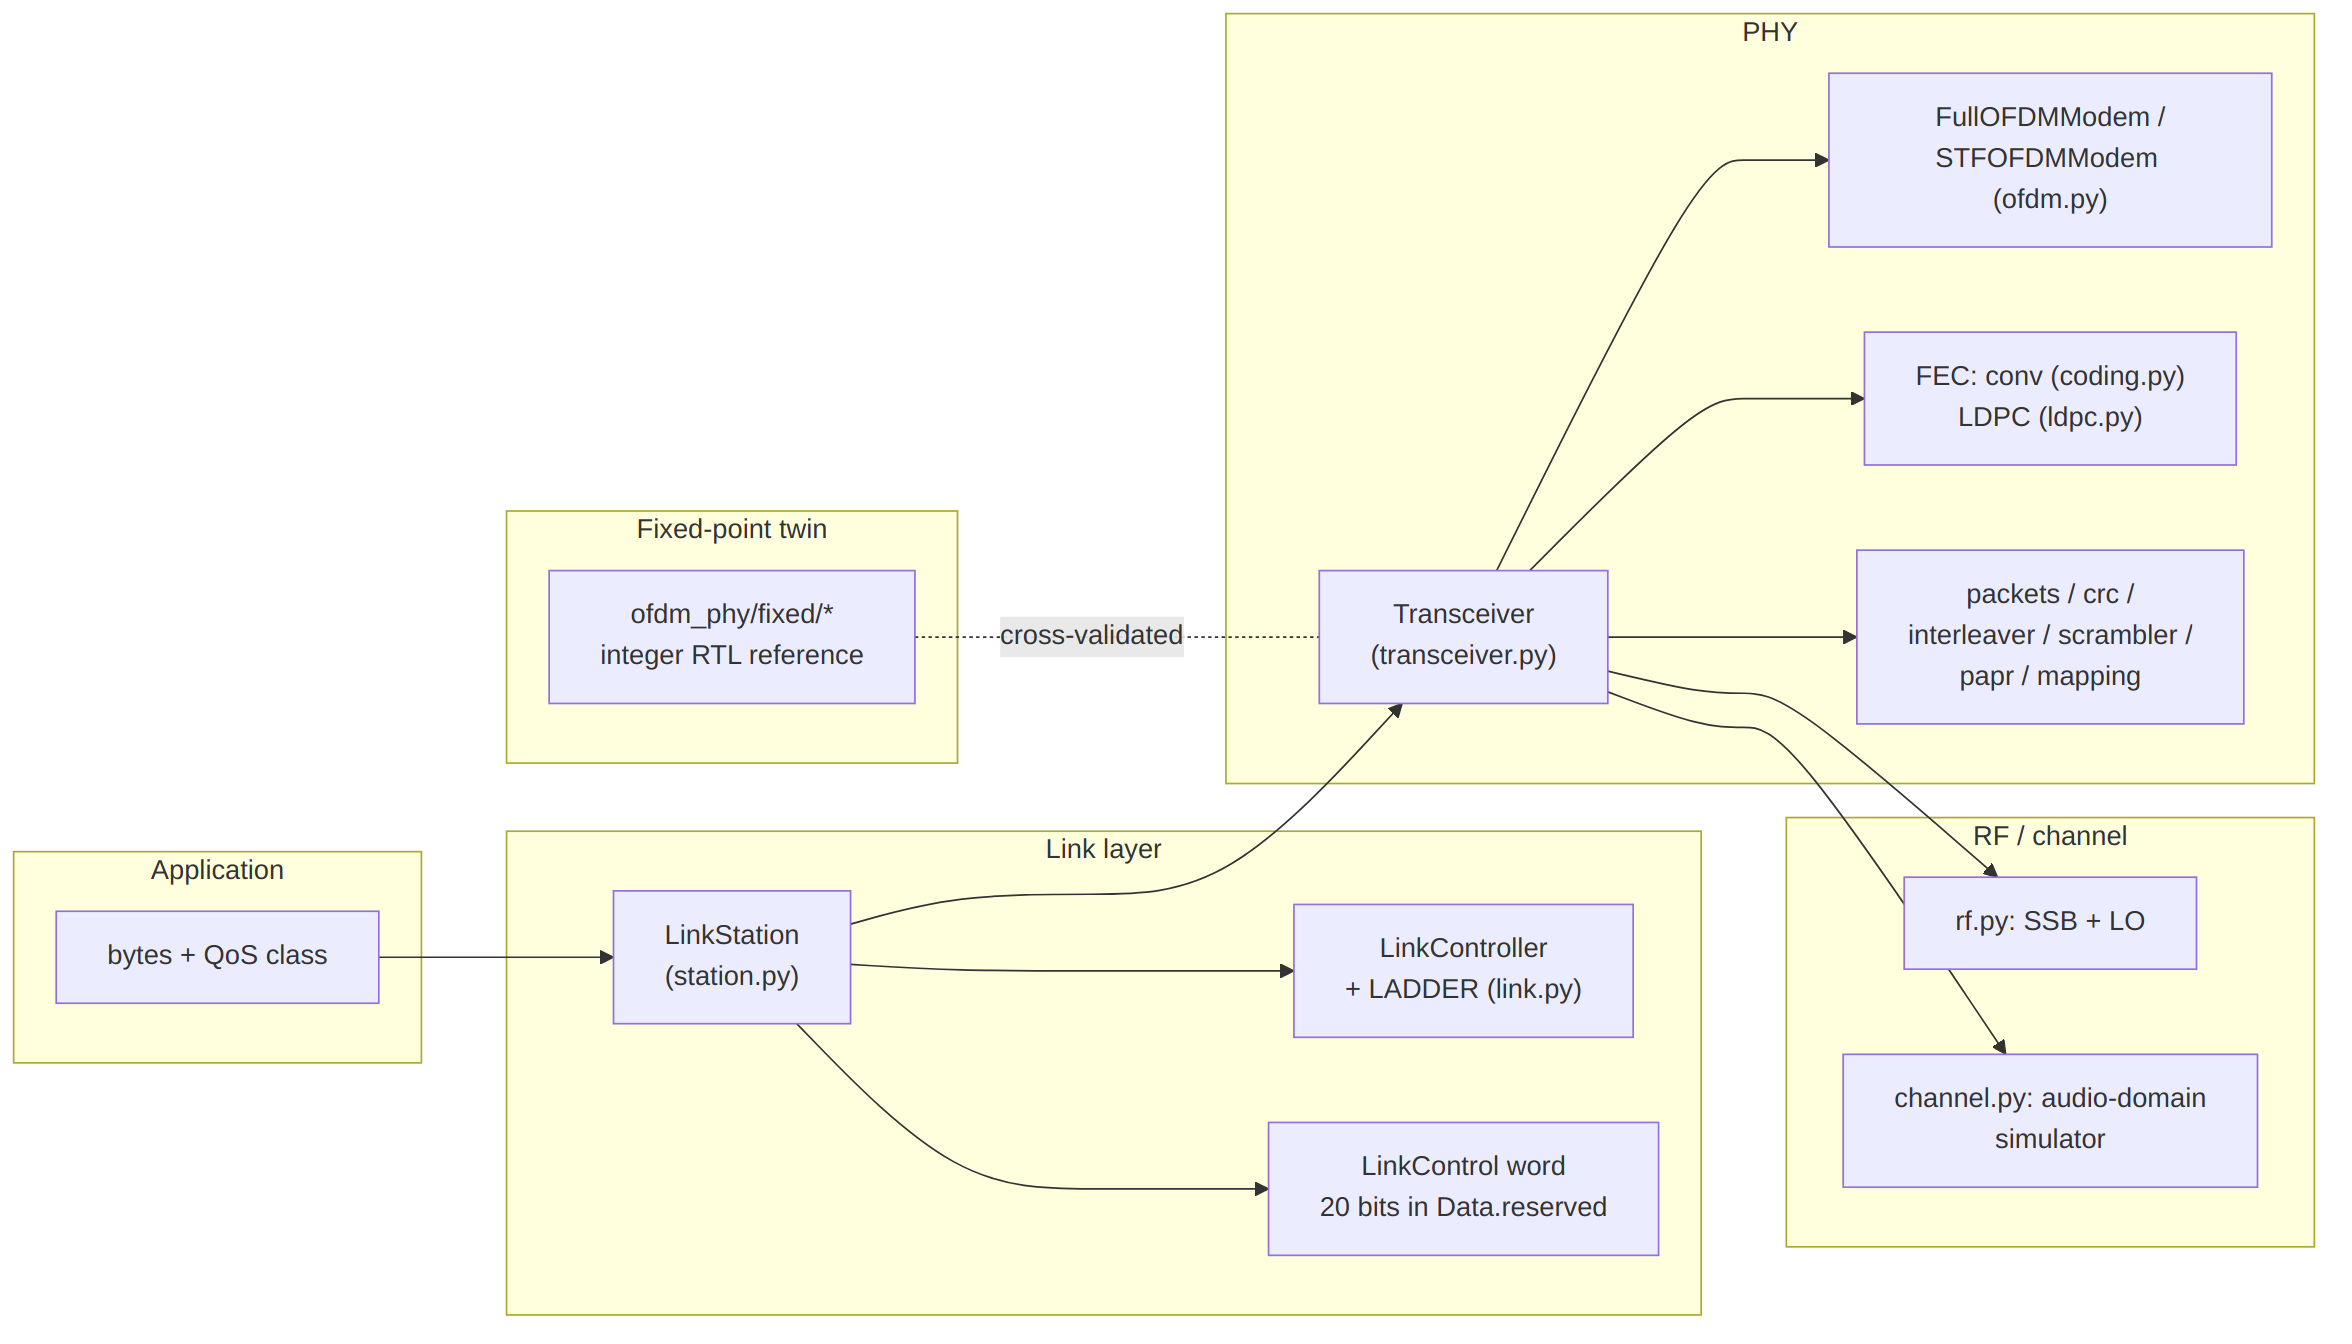
\includegraphics[width=\textwidth,height=0.55\textheight,keepaspectratio]{images/arch_layers.png}
    \caption{Layered architecture of the prototype.  The simulation-side
             layers (\texttt{channel.py}, \texttt{rf.py}) are exactly
             what a real deployment replaces with a soundcard and an SSB
             transceiver.}
    \label{fig:arch_layers}
\end{figure}

Three design principles shaped every layer.  First, \emph{faithful
defaults}: the plain \texttt{Transceiver} reproduces the article's
behaviour exactly (convolutional FEC, raw LLRs), and every improvement
--- LLR recalibration, LDPC coding, HARQ, AFC --- is opt-in and enabled
at the link layer, so the article-reproduction experiments remain valid
permanently.  Second, \emph{self-describing frames}: each link mode
owns a distinct Zadoff--Chu preamble root, so the receiver identifies
the mode from the preamble itself and a mode switch can never deadlock
the link.  Third, \emph{everything measured feeds back}: per-frame SNR
drives rate adaptation, per-frame CFO drives AFC netting, failed
decodes export their LLRs for HARQ combining, and every ACK or timeout
nudges learned per-rung sensitivity offsets.

\subsection{Scope of This Report}

This report documents the complete prototype in
\texttt{ofdm\_transceiver\_proto}: the article reproduction and its
verification, the synchronization analysis that closed the sensitivity
gap, every subsequent extension of the waveform and the link layer,
the two implementations that followed the Python model, and what the
system did on real hardware --- two boards on a wire, a
software-defined radio, and voice.  All quantitative claims are backed
by scripts in \texttt{experiments/} or by a bench target in
\texttt{cport/} (Section~\ref{sec:results}), and every one is
measured on a channel defined in Section~\ref{sec:channels}; the
measured artefacts (curves, JSON sweeps, WAV recordings) live in
\texttt{results/}.  Developer-oriented documentation with the same
structure exists as Markdown with Mermaid diagrams in \texttt{docs/}:
the layer documents (architecture, PHY, link, RF, fixed-point)
alongside four interface documents written for whoever implements
\emph{against} the system rather than inside it --- the channel
drivers, the two consoles, the USB transport, and the modem's
command/event model (Section~\ref{sec:cport_docs}).

\subsection{Contributions}

\begin{itemize}
    \item \textbf{Bit-exact article reproduction} --- 44/44 worked
          examples verified; BER/PER curves (article Figures~23--24)
          reproduced on the article's channel model; measured
          sensitivity $-7.2$\,dB versus the article's
          $\approx-7.5$\,dB, with the residual attributed to
          synchronization by a genie-synchronized control measurement.
    \item \textbf{Synchronization analysis and repair} --- three
          defects identified and fixed: the Zadoff--Chu
          time--frequency ambiguity ($\sim$1\,dB), an SNR-dependent
          tone-detection metric, and a preamble transmitted 7\,dB
          below data power.  An alternative 802.11-style preamble
          (proposed in the article's comment thread) was implemented
          and shown statistically equivalent.
    \item \textbf{SNR-adaptive modes} --- $16\times$ and $64\times$
          tiling modes with per-symbol residual-CFO hypothesis search,
          group-coherent ZC detection, and per-mode preamble roots,
          extending the sensitivity floor to $-17.9$\,dB (78\,\% of
          Shannon capacity at $-20$\,dB).
    \item \textbf{LLR recalibration} --- a measured monotone
          reliability map correcting a shape (not temperature)
          miscalibration of the demodulator's LLRs, worth 1.5--2\,dB
          at the BPSK/QPSK sensitivity edge.
    \item \textbf{Coding and modulation extensions} --- an IRA LDPC
          code (N=768, K=256) with normalized min-sum decoding,
          Gray-mapped 16-QAM extending the ladder to $+4.7$\,dB and
          1059\,bit/s, and CRC-gated chase-combining HARQ.
    \item \textbf{Adaptive link layer} --- a 13-rung measured rate
          ladder, receiver-driven adaptation over a 20-bit piggybacked
          link-control word, QoS with fragment-boundary preemption,
          stop-and-wait ARQ, and simplex channel access with carrier
          sense; validated by a whole-system two-station test with a
          mid-transfer fade.
    \item \textbf{AFC frequency netting} --- closed-loop carrier
          netting through the LC word ($+284$\,Hz initial offset
          converged inside a 12\,Hz deadband in five exchanges), with
          trim-budget and anchor guard rails against common-mode
          frequency drift.
    \item \textbf{RF-chain simulator} --- SSB modulator/product
          detector at a 48\,kHz IF rate with one shared reference
          oscillator per station, making CFO emerge physically from
          ppm errors and thermal drift (validated to 0.1\,Hz).
    \item \textbf{Fixed-point RTL reference model} --- an integer-only
          receiver covering the full frame family (conv+LDPC,
          BPSK/QPSK/16-QAM, all modes, HARQ, calibrated LLRs), within
          0.5\,dB of the float receiver at $-7$\,dB and ahead of it at
          $-9/-10$\,dB; its two-lag CFO unwrap recovered $\sim$8\,\%
          of all acquisitions that ARQ had been hiding.
    \item \textbf{Bit-exact C implementation on a microcontroller} ---
          the whole stack in C99 with no allocation and no floating
          point on the signal path, verified byte for byte against
          golden vectors; a streaming receiver whose memory follows the
          signal rather than the capture (10\,MB $\to$ 561\,KB, flash
          242 $\to$ 57\,KB); the EXTREME acquisition brought from
          not keeping up to 9.5\,\% of a 480\,MHz Cortex-M7 by
          measurement on the part; selective-repeat bursts, streamed
          windows, a capability handshake and operator ceilings ---
          68\,kB across the wire at 87\,\% of the raw rung-12 rate.
    \item \textbf{Two boards that are radios} --- flash-resident
          firmware with a 12\,kHz converter path, carrier sense with a
          DC-blind front end hardened by a stress campaign, a USB
          vendor-class modem protocol with a specification, and the
          field findings that shaped the link layer: a sentinel that
          crossed the air, a reply timer that had to learn the
          end-of-frame commit, a broadcast rung that decides who can
          hear it.
    \item \textbf{Adaptive broadcast} --- non-acknowledged delivery
          with a sender-signalled statistics exchange that re-rungs
          between blocks, proven on a fading harness ($+32$--39\,\% of
          the stream delivered against a held rung) and on the wire;
          a 73\,kB file byte-identical with 0 of 3089 frames lost.
    \item \textbf{Hosts on the link} --- a KISS TNC and an IP tunnel,
          each admitting traffic by air time rather than length; the
          SDR path with the transmitted spectrum, drive limits and an
          off-air decode measured; and a receive chain calibrated
          against a reference source.
    \item \textbf{Voice at 250\,bit/s} --- a neural codec evaluated
          for domain sensitivity, speaker identity, enrolment cost and
          streaming, then put on the air with push-to-talk between the
          boards: first audio 3.6\,s after the talker starts, decoded
          as it arrives, 24 of 24 transmissions lossless once a
          receiver commit defect the mode alone could expose was fixed.
\end{itemize}


\subsection{Signal Profile at a Glance}
\label{sec:signal_profile}

Table~\ref{tab:signal_profile} summarizes the on-air appearance of the
waveform in the style of a signal-identification database
entry~\cite{sigidwiki_vara}, for quick comparison with established
sound-card HF modes such as VARA~HF.

\begin{table}[H]
    \centering
    \caption{Signal identification profile (sigidwiki-style summary).}
    \label{tab:signal_profile}
    \small
    \begin{tabular}{@{}lp{9.2cm}@{}}
    \toprule
    \textbf{Field} & \textbf{Value} \\
    \midrule
    Frequency range   & any SSB voice channel (the waveform lives in the
                        300--2400\,Hz audio passband); amateur HF in the
                        source article's context \\
    Mode              & USB (audio passband, AGC off) \\
    Modulation        & OFDM, 23 subcarriers (16 data + 7 Zadoff--Chu
                        pilots), BPSK / QPSK / 16-QAM \\
    FEC               & convolutional $K{=}7$ rate 1/3 punctured to
                        1/2, 2/3, 3/4 (soft Viterbi); optional IRA LDPC \\
    Bandwidth         & $\approx$2.1\,kHz occupied (bins 3--25 at
                        93.75\,Hz spacing) \\
    Symbol rate       & 22.1 / 5.8 / 1.46\,symbols/s
                        (NORMAL / ROBUST / EXTREME tiling) \\
    ACF               & 10.7\,ms (intra-symbol tile);
                        45.3 / 173 / 685\,ms (symbol, mode-dependent) \\
    Net data rate     & 7.8--1059\,bit/s, 13-rung adaptive ladder
                        (Table~\ref{tab:ladder}) \\
    Sensitivity       & down to $-17.9$\,dB SNR (noise in the 6\,kHz
                        Nyquist band; $\approx-14$\,dB re 2.5\,kHz) \\
    Identification    & three-part preamble: two Newman-phased tone
                        combs, then a tiled Zadoff--Chu symbol whose
                        root (17/19/21) labels the link mode; the
                        EXTREME bootstrap is heard as a
                        $\approx$21\,s steady warble \\
    Duplex / access   & simplex; carrier sense, stop-and-wait ARQ with
                        selective-repeat streamed bursts, capability
                        handshake, and a non-acknowledged broadcast
                        mode (Sections~\ref{sec:link},
                        \ref{sec:broadcast}) \\
    Status            & research prototype (this work): simulation,
                        two-board wire stand, and an off-air decode
                        through an SDR at 7\,MHz; not a deployed
                        on-air standard \\
    Short description & audio-band adaptive OFDM data modem for SSB
                        transceivers, reproducing and extending the
                        PHY of~\cite{habr_ofdm} \\
    \bottomrule
    \end{tabular}
\end{table}

\subsection{Report Structure}

Section~\ref{sec:channels} defines the conventions and the six
channels --- three simulated, one wired, one radio, one a family of
harnesses --- on which everything that follows was measured, and maps
each headline result to its channel.

Part~\ref{part:phy} is the physical layer.
Section~\ref{sec:phy} describes the PHY as implemented;
Section~\ref{sec:sync} the synchronization analysis that closed the
sensitivity gap; Section~\ref{sec:modes} the SNR-adaptive link modes;
Section~\ref{sec:llr} LLR quality measurement and recalibration; and
Section~\ref{sec:coding} the LDPC, 16-QAM and HARQ extensions.

Part~\ref{part:link} is the link layer.  Section~\ref{sec:link}
covers the rate ladder, the link-control word, adaptation, ARQ and
QoS, burst windows, the reply timer, simplex access, the capability
handshake and AFC netting; Section~\ref{sec:broadcast} the broadcast
mode, from its design on the simulated channels to the statistics
exchange the boards required.

Part~\ref{part:impl} is the implementations and what they did.
Section~\ref{sec:fixed} is the fixed-point RTL reference model;
Section~\ref{sec:cport} the C implementation as engineering ---
bit-exactness, the streaming receiver, memory and processor budgets,
hardening; Section~\ref{sec:radio} the radio firmware and the
two-board stand; Section~\ref{sec:host} the USB interface and the host
tools; Section~\ref{sec:cport_sdr} the SDR path; and
Section~\ref{sec:cport_voice} voice at 250\,bit/s, evaluated and then
on the air.

Part~\ref{part:results} consolidates.  Section~\ref{sec:results}
collects the regression suites, the measured gains and the
demonstrations; Section~\ref{sec:discussion} discusses what binds
performance, the limitations and the work ahead; and
Section~\ref{sec:conclusion} concludes.

\section{PHY Layer}
\label{sec:phy}

\subsection{Numerology}

The waveform is designed to pass through an ordinary SSB transceiver's
audio path (AGC off).  Table~\ref{tab:numerology} lists the parameters,
all taken from the article~\cite{habr_ofdm}.

\begin{table}[H]
    \centering
    \caption{OFDM numerology.}
    \label{tab:numerology}
    \small
    \begin{tabular}{@{}lp{8.5cm}@{}}
    \toprule
    \textbf{Parameter} & \textbf{Value} \\
    \midrule
    Sample rate       & 12\,kHz \\
    FFT size          & 128 bins $\rightarrow$ 93.75\,Hz subcarrier spacing \\
    Occupied band     & 300--2400\,Hz $\rightarrow$ bins 3--25, 23 subcarriers \\
    Pilots            & 7, Zadoff--Chu root 3, bins 3, 6, 10, 14, 17, 21, 25 \\
    Data carriers     & 16 \\
    Cyclic prefix     & 32 samples (25\,\%) \\
    Symbol tiling     & $4\times$ / $16\times$ / $64\times$ by link mode
                        (+6\,dB per $4\times$, coherent) \\
    CFO tolerance     & $\pm$375\,Hz design, $\pm$300\,Hz specified \\
    \bottomrule
    \end{tabular}
\end{table}

Symbol \emph{tiling} is the article's central trick for negative-SNR
operation: each OFDM symbol body is repeated back-to-back
\texttt{sym\_tile} times, and the receiver accumulates the repeats
coherently before the FFT.  Each $4\times$ factor buys $\approx$6\,dB
of effective SNR at a $4\times$ rate cost.

\subsection{Frame Structure}

Every frame (Figure~\ref{fig:frame_structure}) carries a two-stage
preamble --- Newman-phased tone combs~\cite{newman1965} for detection
and coarse CFO, then Zadoff--Chu symbols for sample-exact timing ---
followed by a header and the data block.  The header (25 bits:
\texttt{ver(2)\,|\,typ(3)\,|\,mod(2)\,|\,spd(2)\,|\,len(8)\,|\,CRC-8})
is always sent in the most robust configuration (BPSK, rate-1/3, six
tiled symbols = 93 coded bits); its \texttt{mod}/\texttt{spd}/%
\texttt{len} fields drive the data-block demodulation, and
\texttt{ver=2} marks an LDPC-coded data block
(Section~\ref{sec:coding}).  Preamble bins carry deliberate gain
($\times 2$ for ZC symbols, $\times\sqrt{5.75}$ for tone combs) so the
whole frame has uniform per-sample power --- Section~\ref{sec:sync}
shows why detection sensitivity depends on this.

\begin{figure}[H]
    \centering
    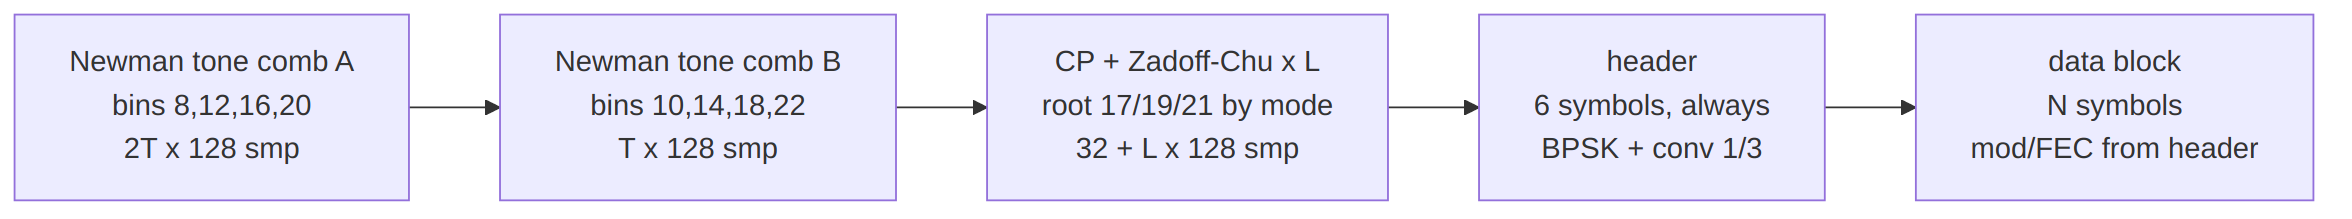
\includegraphics[width=\textwidth]{images/frame_structure.png}
    \caption{Frame structure.  $T$ is the mode's tone-tiling factor and
             $L$ the mode's Zadoff--Chu symbol count.}
    \label{fig:frame_structure}
\end{figure}

\subsection{Transmit Chain}

Figure~\ref{fig:tx_chain} shows the transmit chain
(\texttt{Transceiver.build\_frame}).  Packet bits (with CRC) are
FEC-encoded, zero-padded to a whole number of OFDM symbols
\emph{before} interleaving, interleaved over the 16 data carriers,
scrambled by a 15-bit LFSR, mapped (BPSK/QPSK/16-QAM Gray), and
assembled into OFDM symbols with the ZC pilots and a Hermitian mirror
so the time-domain signal is real.  After tiling and CP insertion the
preamble is prepended and a clip-and-filter stage (clip at
RMS+6\,dB, low-pass at 3\,kHz) bounds the PAPR.

\begin{figure}[H]
    \centering
    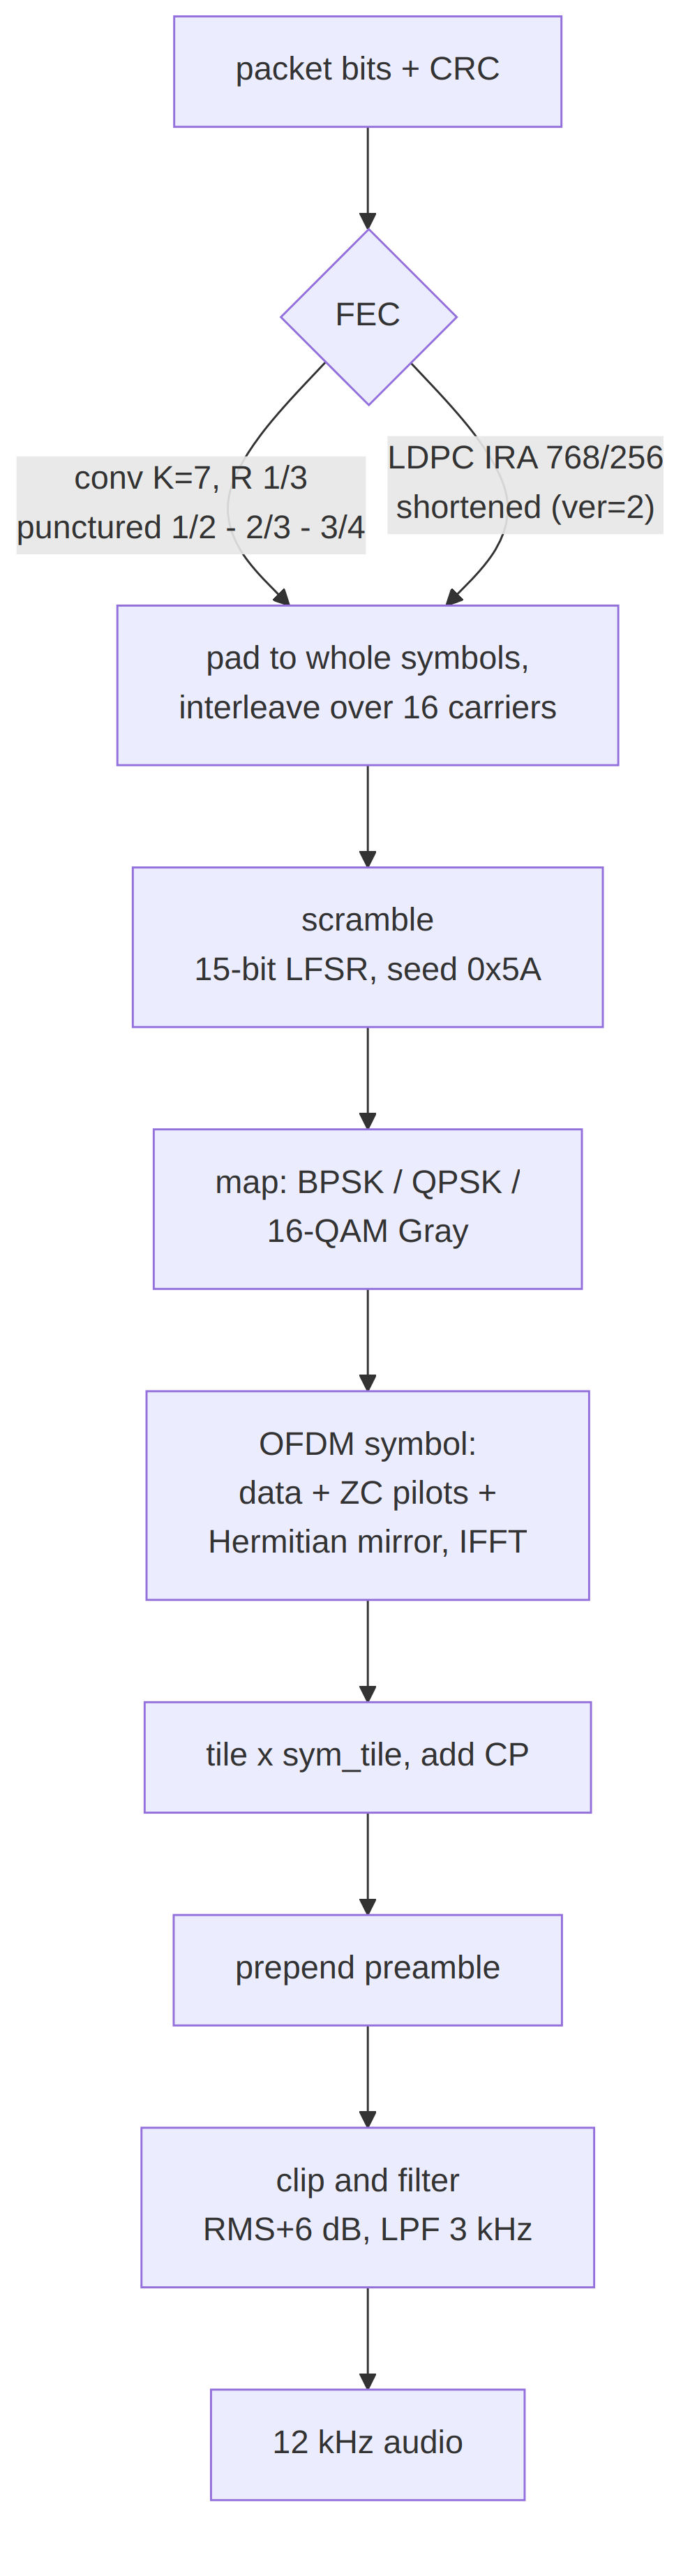
\includegraphics[width=0.62\textwidth,height=0.55\textheight,keepaspectratio]{images/tx_chain.png}
    \caption{Transmit chain.}
    \label{fig:tx_chain}
\end{figure}

Two ordering invariants are easy to break and worth stating: TX applies
interleave \emph{then} scramble, so RX must descramble \emph{then}
deinterleave; and because the FEC block is padded to whole symbols
before interleaving, RX must crop the deinterleaved stream back to the
codec's block length before decoding.

\subsection{Receive Chain}

Figure~\ref{fig:rx_chain} shows the receive chain
(\texttt{Transceiver.demod\_frame}).  After the analytic-signal
transform, synchronization runs in three stages (detailed in
Section~\ref{sec:sync}); the demodulator then processes each tiled
symbol: CP removal and coherent tile accumulation (with per-symbol
phase tracking), FFT, pilot-based channel estimation (zero-forcing
estimate at the pilots, Wiener smoothing with an exponential
frequency-correlation model of length 8 bins, MMSE equalization), and
LLR formation weighted by the per-carrier symbol SNR, clipped to
$\pm 20$.  One convention is load-bearing across four modules: LLR
sign is \textbf{positive = logical 1}, consistent with the article's
BPSK mapping table (the article's prose states the opposite of its own
code).

\begin{figure}[H]
    \centering
    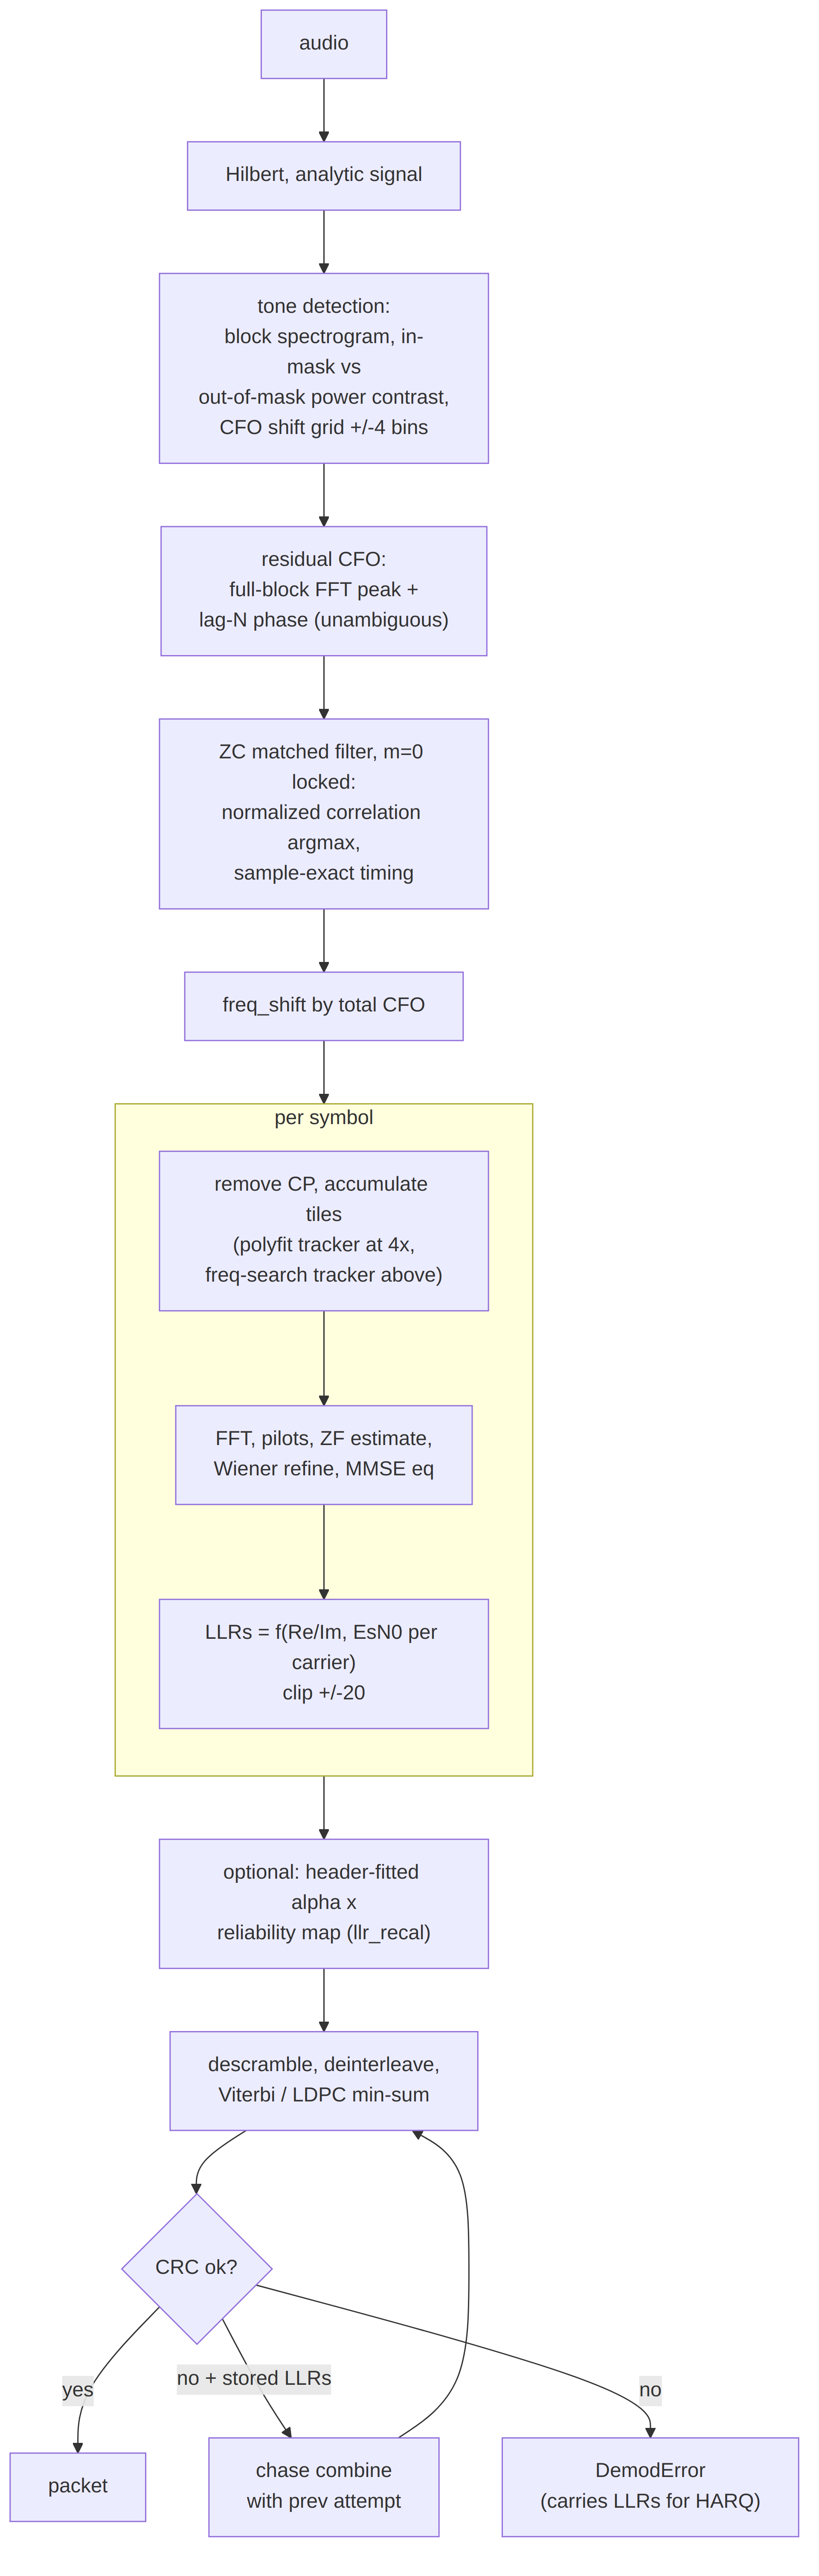
\includegraphics[width=0.72\textwidth,height=0.6\textheight,keepaspectratio]{images/rx_chain.png}
    \caption{Receive chain, including the opt-in recalibration stage
             (Section~\ref{sec:llr}) and the HARQ path
             (Section~\ref{sec:coding}).}
    \label{fig:rx_chain}
\end{figure}

A CRC failure does not simply discard the frame: the
\texttt{DemodError} exception carries the decoded header and the
data-block LLRs, which is what makes the chase-combining HARQ of
Section~\ref{sec:coding} possible without any extra signalling.

\subsection{Soft Demodulation: from Symbols to LLRs}
\label{sec:llr_math}

This subsection states exactly what the demodulator computes
(\texttt{OFDMModem.demodulate\_symbol\_cp\_soft}).  After tile
accumulation and FFT, each data carrier $k$ of a symbol obeys
\begin{equation}
    Y_k = H_k S_k + N_k,
    \qquad N_k \sim \mathcal{CN}(0, \sigma^2),
\end{equation}
where $H_k$ is the channel coefficient and $S_k$ the transmitted
constellation point.  With $\hat{H}_k$ the Wiener-smoothed pilot
estimate, the MMSE equalizer output is
\begin{equation}
    \hat{S}_k \;=\;
    \frac{Y_k\,\hat{H}_k^{*}}{|\hat{H}_k|^{2} + \hat{\sigma}^{2}} .
    \label{eq:mmse}
\end{equation}
The noise power $\hat\sigma^2$ is tracked decision-directed: the
mean-square error of $\hat S_k$ against the nearest constellation
point (per axis for BPSK/QPSK; against the sliced 16-QAM grid for
$\mu=4$), referred back through the channel by the mean
$|\hat H_k|^2$, and smoothed with an exponential filter
($\alpha = 0.1$) across symbols.  The per-carrier symbol SNR
\begin{equation}
    \rho_k \;=\; \frac{|\hat{H}_k|^{2}}{\hat{\sigma}^{2}}
\end{equation}
weights every LLR, so bits on faded carriers enter the decoder as
weak evidence rather than as confident errors.

The log-likelihood ratio of a bit $b$ is defined here as
\begin{equation}
    L(b) \;=\;
    \ln \frac{P(b = 1 \mid \hat{S})}{P(b = 0 \mid \hat{S})},
\end{equation}
i.e.\ \textbf{positive LLR means logical~1} --- the load-bearing sign
convention noted above.  Under the max-log approximation
$\ln \sum_i e^{x_i} \approx \max_i x_i$, the general form
\begin{equation}
    L(b_i) \;\approx\; \rho_k
    \Bigl( \min_{s \in \mathcal{S}_0^{(i)}} |\hat{S}_k - s|^2
         - \min_{s \in \mathcal{S}_1^{(i)}} |\hat{S}_k - s|^2 \Bigr)
\end{equation}
collapses to closed forms per modulation (as implemented; overall
scale is immaterial to the scale-invariant Viterbi and min-sum
decoders, but the \emph{shape} across carriers and bit positions is
what Section~\ref{sec:llr} calibrates):
\begin{align}
    \text{BPSK:}\quad
        & L = 4\,\rho_k \operatorname{Re}\hat{S}_k, \\
    \text{QPSK:}\quad
        & L_I = 2\,\rho_k \operatorname{Re}\hat{S}_k,
    \qquad L_Q = 2\,\rho_k \operatorname{Im}\hat{S}_k, \\
    \text{16-QAM (Gray, unit } a = g/\sqrt{10}\text{):}\quad
        & L_{b_0} = 2\,\rho_k \operatorname{Re}\hat{S}_k / g,
    \qquad L_{b_1} = 2\,\rho_k
        \bigl(2a - |\operatorname{Re}\hat{S}_k|\bigr) / g,
    \label{eq:qam_llr}
\end{align}
with the imaginary-axis pair $L_{b_2}, L_{b_3}$ analogous, and $g$ the
per-symbol gain estimate.  The 16-QAM forms are the piecewise-linear
max-log metrics of the Gray mapping: the outer bit ($b_0$) is the axis
sign, the inner bit ($b_1$) discriminates inner from outer amplitude
levels, changing sign at $|\!\operatorname{Re}\hat S| = 2a$.  All LLRs
are clipped to $\pm 20$ before decoding.

\section{Synchronization and the Sensitivity Gap}
\label{sec:sync}

The decode chain reproduced the article bit-exactly almost immediately;
the measured \emph{sensitivity} did not.  This section documents the
diagnosis --- the most instructive part of the reproduction --- and the
resulting synchronizer.

\subsection{Diagnosis Method}

The tool was a \emph{genie-synchronized} control receiver: the same
demodulator fed the true timing offset and CFO from the channel
simulator.  With genie sync the chain measured $-7.6$\,dB (BPSK
rate-1/3, article channel, PER $\le 10\,\%$)\footnote{All
sensitivities in this report use the article's SNR convention: noise
counted across the full 6\,kHz Nyquist band, of which the signal
occupies $\approx$2.1\,kHz.  Add $\approx$4.5\,dB to compare against
in-band noise only, $\approx$3.8\,dB for the ham 2.5\,kHz
convention.}; the real receiver
initially sat several dB worse.  Every improvement below was validated
by closing part of that gap, and the final residual is $\sim$0.3\,dB
(Section~\ref{sec:results}).

\subsection{Three Defects and Their Fixes}

\paragraph{Preamble power.}  Transmitting the tone combs and ZC symbols
at nominal bin amplitude leaves the preamble region $\sim$7\,dB below
the frame-average power (4 tones versus 23 loaded carriers).  Detection
then fails at SNRs where the payload would decode.  The fix is the
gain scaling of Section~\ref{sec:phy}: $\times\sqrt{5.75}$ on tone
bins and $\times 2$ on ZC bins equalizes per-sample power across the
frame.

\paragraph{Tone-detection metric.}  The article's tone detector
thresholds the in-mask energy \emph{fraction} of a block spectrogram.
That fraction is SNR-dependent --- it fails below $\approx$0\,dB
regardless of threshold --- and divides by zero on noise-free signals.
The implemented metric is a \emph{contrast ratio}: mean in-mask bin
power over mean out-of-mask bin power, evaluated over a grid of
$\pm 4$-bin CFO shifts of the mask, with the denominator regularized
by 1\,\% of the median block power.  The regularizer matters: on clean
signals the out-of-mask power is $\approx$0 and the unregularized
argmax degenerates into a lottery among CFO hypotheses, producing exact
one- and two-bin CFO errors on clean WAV recordings.

\paragraph{Zadoff--Chu time--frequency ambiguity.}  The ZC matched
filter selects the best \emph{normalized} correlation over a search
window after the tone preamble (the raw-peak argmax locks onto the
periodic tiled data symbols).  The subtler defect was scanning the ZC
correlation over $\pm 1$-bin frequency hypotheses: a Zadoff--Chu
sequence's frequency-shifted replica correlates almost as well at a
\emph{shifted time} (the classic ZC time--frequency ambiguity), so at
low SNR the wrong hypothesis wins, injecting a one-subcarrier
(93.75\,Hz) CFO error plus a $\sim$30-sample timing error.  Locking
the composite detector to the zero-CFO hypothesis --- legitimate
because the tone stage already leaves a residual well below half a bin
--- recovered $\approx$1\,dB of sensitivity by itself.

\paragraph{Residual CFO.}  The tone-stage residual CFO is estimated by
a full-length FFT peak over the first tone block (unambiguous over
$\pm 1.5$ bins), refined by a lag-$N$ phase estimate.  A lag-$N$
estimate alone is ambiguous modulo one subcarrier spacing; during
development a lag-16 variant produced 276\,Hz errors because the lag
was not a multiple of the tone-comb period --- the general rule
(enforced in the code) is that a delay-and-correlate lag must be a
multiple of the comb's time-domain period.

\subsection{The STF Preamble Variant}

A commenter on the article proposed replacing the Newman tone comb with
802.11-style short-training tones every 8 bins.  This was implemented
as \texttt{STFOFDMModem}: tone combs on bins $[8,16,24]$ and
$[4,12,20]$ make the tone block periodic with 16 samples, so the
residual CFO comes from a plain Schmidl--Cox-style
delay-and-correlate~\cite{schmidl1997} (lag 16 refined by lag 128),
unambiguous over $\pm 375$\,Hz.  An A/B sweep over the full
$\pm 300$\,Hz CFO range and all eight modulation/rate configurations
shows the two preambles statistically equivalent: identical
$-7.2$\,dB sensitivity, all eight per-configuration sensitivities
within 0.14\,dB, every PER point within $2\sigma$ binomial noise
(Figure~\ref{fig:stf_vs_newman}).  The article-faithful
\texttt{FullOFDMModem} remains the default.

\begin{figure}[H]
    \centering
    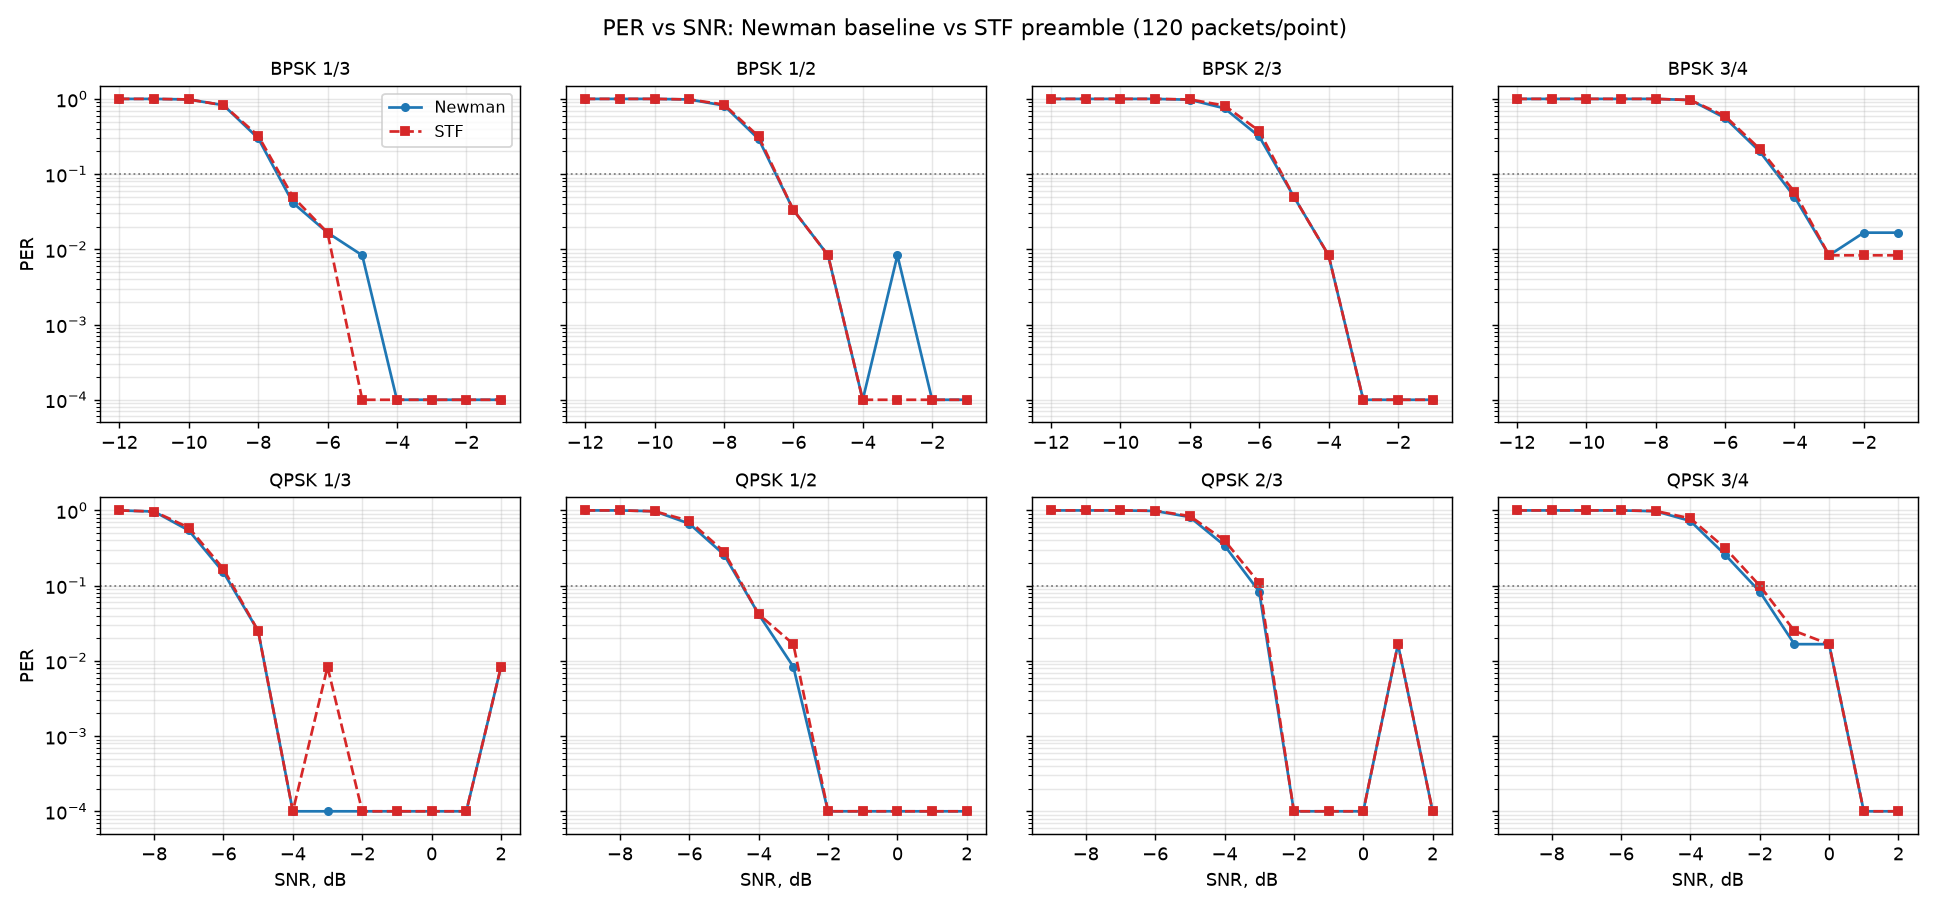
\includegraphics[width=0.9\textwidth]{images/per_stf_vs_newman.png}
    \caption{PER versus SNR for the Newman-tone and STF preamble
             variants over the article channel (same channel
             realizations per arm).}
    \label{fig:stf_vs_newman}
\end{figure}

\section{SNR-Adaptive Link Modes}
\label{sec:modes}

The article's waveform operates around $-7$\,dB.  The first major
extension scales the coherent-accumulation tile factor (and the
preambles with it) into three link modes
(Table~\ref{tab:modes}), trading bitrate for sensitivity.

\begin{table}[H]
    \centering
    \caption{Link modes (sensitivities at PER $\le 10\,\%$,
             recalibrated receiver, article channel, 6\,kHz-band SNR).}
    \label{tab:modes}
    \small
    \begin{tabular}{@{}lrrrr@{}}
    \toprule
    \textbf{Mode} & \textbf{Tiles} & \textbf{ZC root} &
    \textbf{User rate (BPSK 1/3)} & \textbf{Sensitivity} \\
    \midrule
    NORMAL  & $4\times$  & 17 & 118\,bit/s & $-7.6$\,dB \\
    ROBUST  & $16\times$ & 19 & 31\,bit/s  & $-11.7$\,dB \\
    EXTREME & $64\times$ & 21 & 7.8\,bit/s & $-17.9$\,dB \\
    \bottomrule
    \end{tabular}
\end{table}

Shannon capacity~\cite{shannon1948} of the 2100\,Hz occupied band at
$-20$\,dB (6\,kHz reference) is $\approx$30\,bit/s; EXTREME's channel
rate of 22\,bit/s is 78\,\% of capacity, so the theoretical wall for
this bandwidth is $-20.7$\,dB and the measured $-17.9$\,dB floor sits
$\approx$3\,dB from it.

\subsection{What Makes the Low-SNR Modes Work}

Each of the following was found necessary empirically; removing any one
of them collapses the EXTREME mode.

\paragraph{Per-symbol residual-CFO hypothesis search.}  A $64\times$
tiled symbol integrates coherently over 0.69\,s and cannot tolerate
even a few Hz of residual CFO across the accumulation window; per-tile
phase tracking (the NORMAL-mode polynomial fit) is pure noise at
$-19$\,dB.  The tiled demodulator instead derotates the whole symbol
over a grid of frequency hypotheses, accumulates tiles under each, and
keeps the hypothesis with maximum in-band energy --- spending the
symbol's \emph{entire} energy ($\approx$19\,dB $E/N_0$ even at
$-20$\,dB SNR) on the frequency decision.  A slew-limited tracker
(full grid on the first symbol, $\pm 2$ grid steps thereafter)
suppresses per-symbol argmax noise; the search range must cover the
worst-case preamble CFO error ($\pm 25$\,Hz for EXTREME).

\paragraph{Finer detection FFT.}  ROBUST and EXTREME tone detection
uses 512-point spectrogram blocks: $4\times$ more tone energy per bin,
and a 23.4\,Hz coarse-CFO grid whose residual fits a plain lag-$N$
estimate.

\paragraph{Group-coherent ZC correlation.}  The ZC stage correlates
kernels of 2--4 concatenated ZC symbols (magnitudes summed across
groups) with a small fractional-CFO hypothesis grid ($\pm 15$\,Hz) ---
single-symbol correlation is not selective enough at $-18$\,dB, and
Section~\ref{sec:sync}'s ambiguity argument forbids a wide frequency
scan.

\paragraph{Per-mode preamble roots.}  The receiver cannot read the tile
factor from the header, because it needs the tile factor to demodulate
the header.  The mode is therefore signalled by the preamble itself:
each mode owns a distinct ZC root (17/19/21), a wrong-root matched
filter simply does not lock, and \texttt{demod\_frame\_auto} tries the
modes in turn (Figure~\ref{fig:mode_autodetect}).  Detection thresholds
were tuned against noise-only false alarms (0/20 on pure noise, all
modes).

\begin{figure}[H]
    \centering
    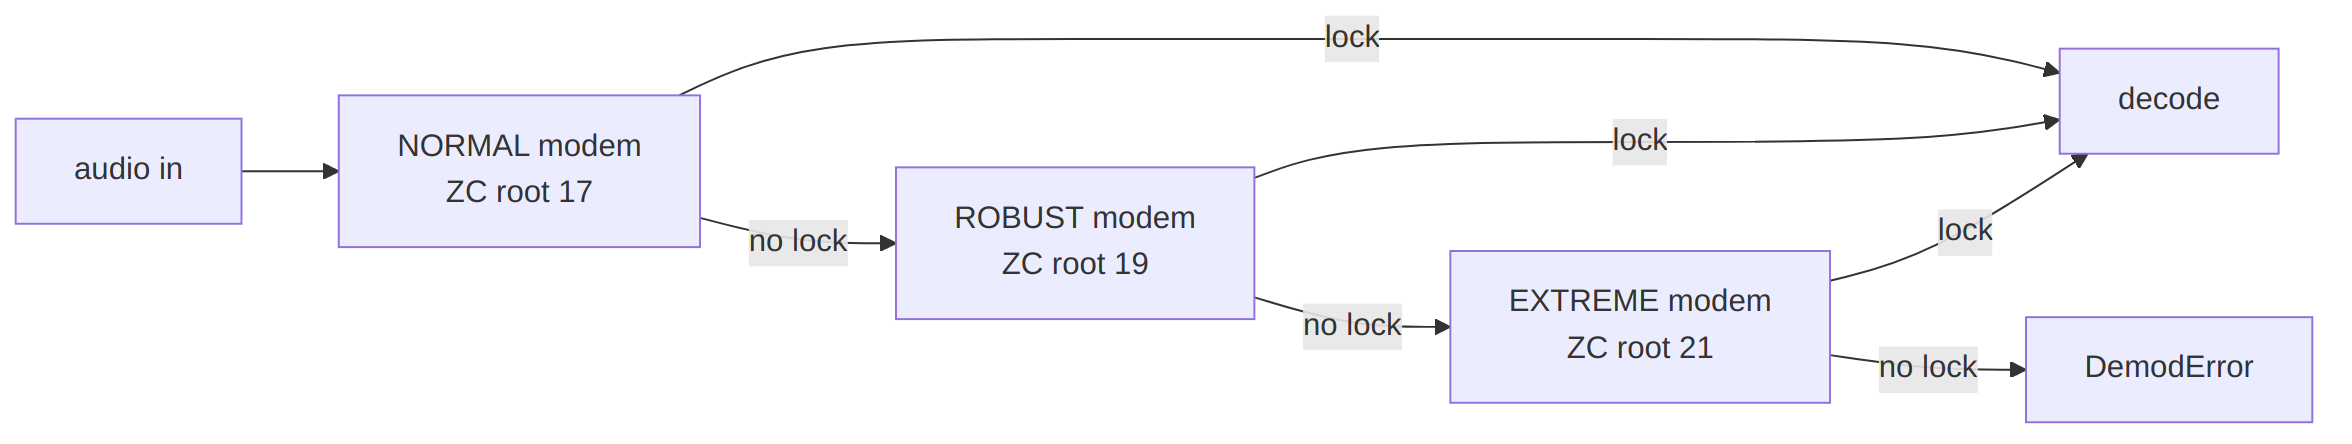
\includegraphics[width=0.9\textwidth]{images/mode_autodetect.png}
    \caption{Blind mode detection: the preamble root \emph{is} the mode
             signal.  A consequence used throughout the link layer: a
             mode switch can never deadlock the link.}
    \label{fig:mode_autodetect}
\end{figure}


\subsection{Constellations Across the Operating Range}

Figure~\ref{fig:const_ladder} makes the adaptation policy visible in
one picture: for eight SNRs spanning the whole operating range
($-17.5$ to $+20$\,dB), it shows the \emph{equalized received
constellation of the rung the rate controller actually selects} at
that SNR (highest rung whose measured sensitivity clears a 1\,dB
margin).  Each panel is produced by the real per-symbol receive chain
--- coherent tiling accumulation, per-symbol frequency search where
the mode uses one, and MMSE equalization
(\texttt{experiments/figures.py}).  At $-17.5$\,dB the EXTREME BPSK
decision variable barely emerges from the noise --- which is precisely
why rung~0 pairs $64\times$ tiling with the rate-1/3 code and soft
decisions; the QPSK quadrants firm up through the mid-ladder, and the
16-QAM grid the top rungs rely on only becomes usable above
$\approx$+3\,dB, matching the ladder sensitivities of
Table~\ref{tab:ladder}.

\begin{figure}[H]
    \centering
    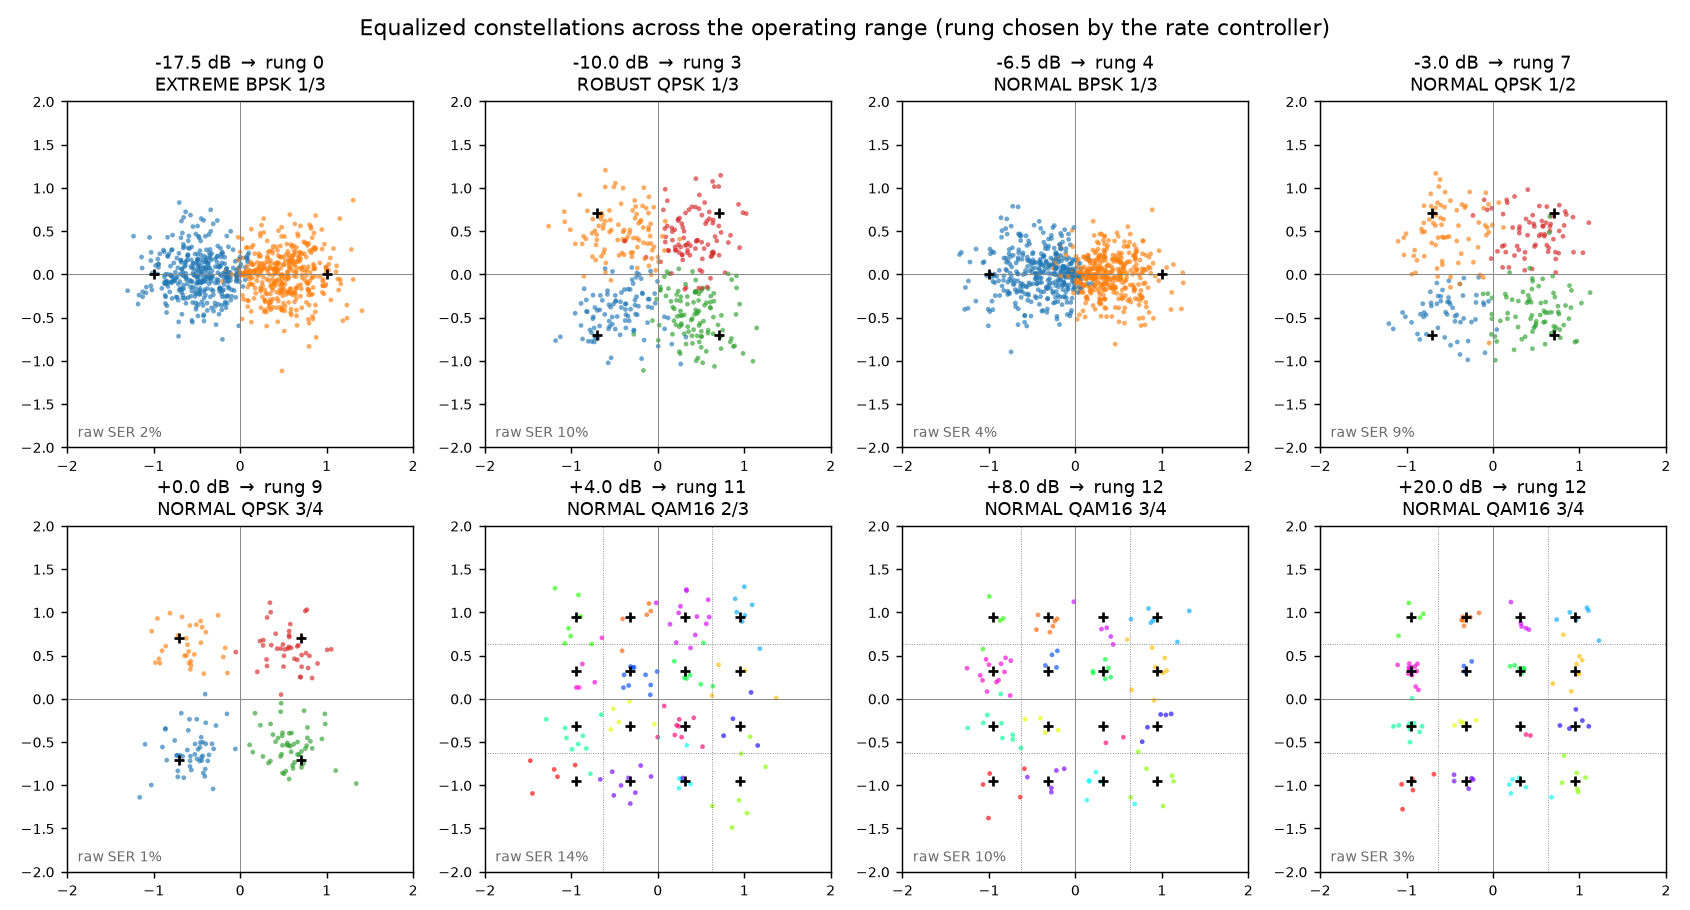
\includegraphics[width=\textwidth]{images/constellation_ladder.png}
    \caption{Equalized constellations at the controller-selected rung,
             from the EXTREME sensitivity floor to a clean channel
             (article channel, AWGN + CFO).  Black crosses mark the
             ideal constellation points; each received point is colored
             by the \emph{transmitted} symbol, so raw pre-FEC errors
             appear as points of the wrong color inside a neighbouring
             decision region (the per-panel ``raw SER'' annotation
             counts them), and the dotted subgrid on the 16-QAM panels
             marks the decision boundaries between the 16 cells.}
    \label{fig:const_ladder}
\end{figure}

\subsection{Measured Waterfalls}

Figure~\ref{fig:adaptive_modes} shows the three modes' PER waterfalls
on the article channel.  The function \texttt{select\_mode} implements
the resulting adaptation policy (mode + modulation + code rate for an
expected SNR), later subsumed by the link-layer ladder of
Section~\ref{sec:link}.

\begin{figure}[H]
    \centering
    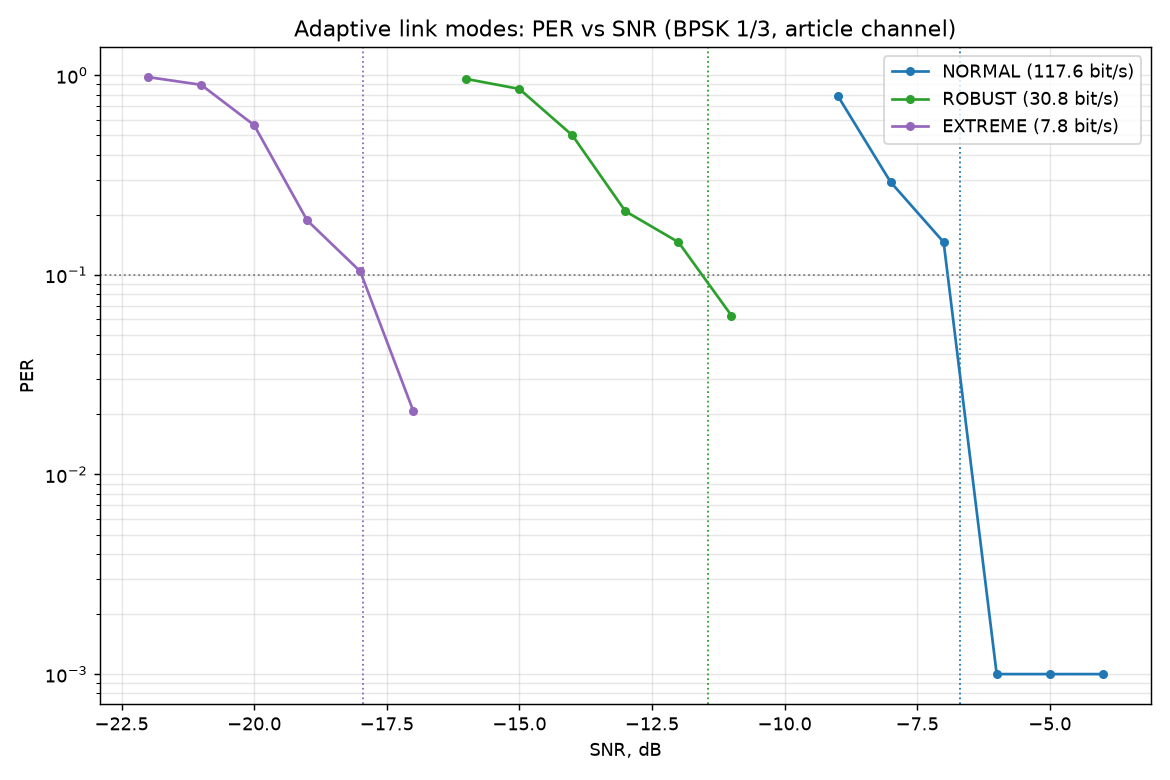
\includegraphics[width=0.9\textwidth]{images/per_adaptive_modes.png}
    \caption{PER versus SNR for the three link modes
             (\texttt{experiments/adaptive\_modes.py}).}
    \label{fig:adaptive_modes}
\end{figure}

\section{LLR Quality and Recalibration}
\label{sec:llr}

A code-review pass over the finished system asked a simple question:
are the demodulator's LLRs actually calibrated --- does $|L|$ mean
what it claims?  Measuring them against ground truth
(\texttt{experiments/llr\_calibration.py}) found the single largest
untapped gain in the system.

\subsection{The Miscalibration Is Shape, Not Temperature}

Two terms are used throughout this section and deserve definition.
\emph{Temperature scaling} is the standard one-parameter recalibration
family
\begin{equation}
    L' \;=\; \alpha \cdot L, \qquad \alpha > 0,
\end{equation}
one global gain applied uniformly to every LLR.  The name comes from
machine-learning calibration~\cite{guo2017calibration}, where a
network's logits are divided by a scalar ``temperature'' $T$ before
the softmax ($\alpha \equiv 1/T$) --- itself borrowed from the
Boltzmann distribution, in which temperature controls how sharply
probability concentrates on the most likely outcome: $\alpha < 1$
softens overconfident beliefs, $\alpha > 1$ sharpens underconfident
ones.  It is the natural first candidate here because it preserves
signs and ordering, costs one multiply, and can be fitted blind on a
per-frame basis: a correctly calibrated Gaussian LLR ensemble
satisfies the consistency condition
$\operatorname{Var}[\ell] = 2\,\mathbb{E}[\ell]$ (for
$\ell = L \cdot \tilde{x}$, the LLR signed by the true bit), so the
moment estimator $\alpha = 2\,\mathbb{E}[\ell]/\operatorname{Var}[\ell]$
recovers the gain that restores consistency.  By contrast,
\emph{shape} refers to any monotone but non-linear correction
$L' = f(|L|) \cdot \operatorname{sgn} L$ --- one that can treat weak
and strong LLRs differently.  The finding of this section is that the
front end's miscalibration is of the second kind, so the first kind
cannot repair it.

The raw LLRs ($4\cdot\mathrm{Re}\cdot E_s/N_0$ per carrier, clipped to
$\pm 20$) are \emph{shape}-miscalibrated: bits with $|L|<2$ err 11\,\%
empirically versus the 39\,\% their value implies --- the
decision-directed noise estimation and per-carrier weighting
over-spread confidence downward --- while the clipped top of the scale
overstates.  A single temperature cannot fix this: the moment fit is
dragged by the clipped mass, and the fitted $\alpha<1$ while the weak
LLRs are empirically \emph{under}confident, a contradiction only a
shape correction resolves.  Figure~\ref{fig:llr_shape} shows the
measured shape.  In the left panel, the measured error rate starts
\emph{below} the ideal curve $P(\mathrm{err}) = 1/(1+e^{|L|})$ (weak
LLRs are better than they claim) and crosses it around $|L| \approx 5$,
after which errors run orders of magnitude \emph{above} the claim ---
and beyond $|L| \approx 9$ the measured reliability actually
\emph{decreases} as the claimed confidence rises, all the way into the
clipped mass at $|L| \approx 19$.
The right panel replots the same data as empirical log-odds versus
nominal $|L|$: a calibrated front end would sit on the identity line,
but the measured curve rises above it at small $|L|$ (wanting
$\alpha > 1$) and falls far below at large $|L|$ (dragging any global
fit to $\alpha < 1$ --- here $\alpha = 0.67$).  No straight line
through the origin can be on the correct side of both regions
simultaneously; the red curve itself, applied as a lookup, is the
monotone reliability map of the next subsection.  Note where the
measured curve peaks: $\approx 7.5$ empirical log-odds at
$|L| \approx 9$ --- the deployed map's cap of $7.4$ is that peak,
re-measured independently.  This is also the
figure that explains the LDPC result of Section~\ref{sec:coding}:
exact sum--product consumes these numbers as \emph{absolute}
probabilities and pays for every lie, while min-sum and Viterbi only
compare them.

\begin{figure}[H]
    \centering
    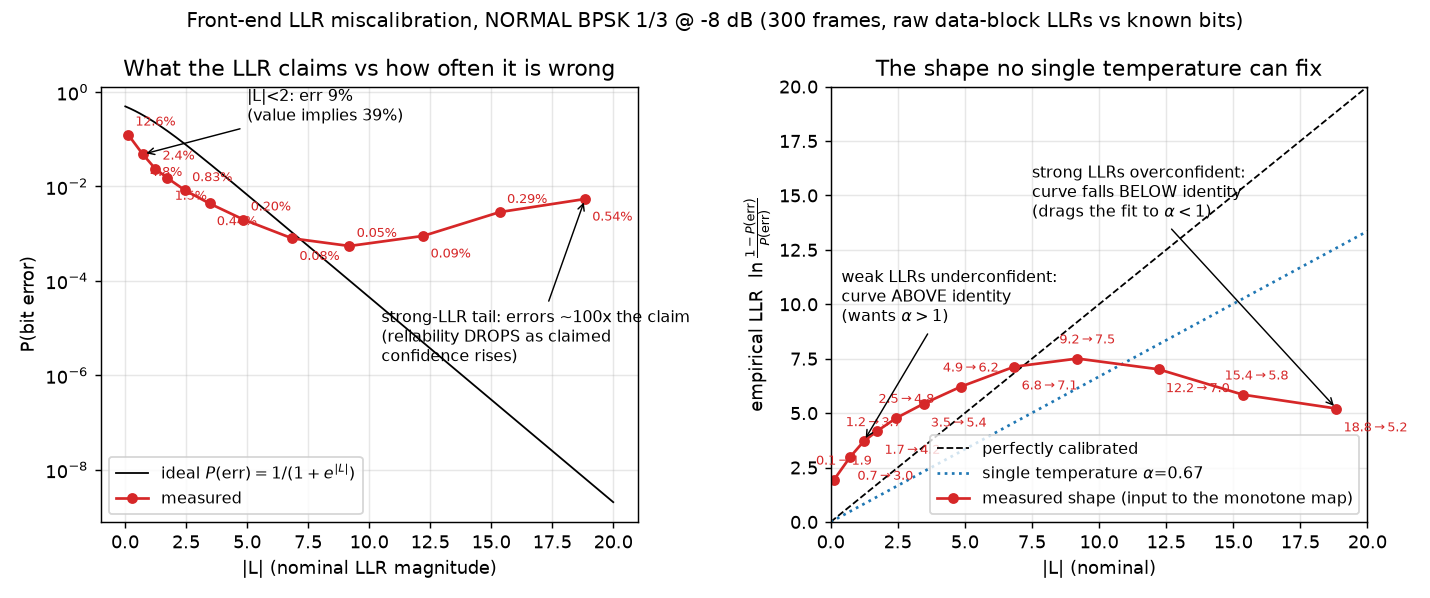
\includegraphics[width=\textwidth]{images/llr_shape.png}
    \caption{The measured LLR miscalibration shape (NORMAL BPSK 1/3
             at $-8$\,dB, 300 frames, raw data-block LLRs against
             known transmitted bits; reproduce with
             \texttt{experiments/llr\_shape.py}, bin table and
             parameters in \texttt{results/llr\_shape.json}).
             Left: claimed versus actual reliability, each bin
             annotated with its measured error rate.  Right: the same
             data as empirical log-odds, each point annotated with its
             mapping (nominal $\rightarrow$ empirical) --- above the
             identity line at small $|L|$, below it at large $|L|$, so
             no single temperature $\alpha$ can correct both ends.}
    \label{fig:llr_shape}
\end{figure}

\subsubsection{Measurement Procedure}
\label{sec:llr_procedure}

The data behind Figure~\ref{fig:llr_shape} (and behind the deployed
map of the next subsection) is produced by a self-labeling protocol
--- the transmitter's bit pipeline is deterministic, so every raw LLR
can be paired with the coded bit it was supposed to carry:

\begin{enumerate}
    \item \textbf{Stimulus.}  300 NORMAL-mode frames, BPSK rate 1/3,
          27-byte random payloads; each passes the channel simulator
          with a random start offset (300--1200 samples), a random
          CFO drawn uniformly from $\pm 60$\,Hz, and AWGN at the
          target SNR ($-8$\,dB here, 6\,kHz convention).  Collection
          runs as parallel 30-frame chunks with per-chunk seeds, so
          the run is reproducible and its result is recorded in
          \texttt{results/llr\_shape.json}.
    \item \textbf{Reception.}  Each frame goes through the
          \emph{production} receive chain --- preamble detection,
          CFO correction, tile accumulation, channel estimation, MMSE,
          LLR formation with the $\pm 20$ clip
          (Section~\ref{sec:llr_math}) --- and the raw data-block
          LLRs are captured \emph{before} any decoding or
          recalibration.  Frames that fail preamble detection are
          skipped; no selection is made on CRC, so decoding failures
          do not bias the sample.
    \item \textbf{Ground truth.}  The known payload is run through
          the TX bit pipeline (FEC encode $\to$ pad $\to$ interleave
          $\to$ scramble), giving the transmitted coded bit for every
          LLR position.  With $\tilde{x} = \pm 1$ ($+1 \Leftrightarrow$
          bit 1, the sign convention), each sample is reduced to the
          signed product $\ell = L \cdot \tilde{x}$: $\ell < 0$ means
          the LLR votes for the wrong bit, and $|\ell| = |L|$ is its
          claimed confidence.
    \item \textbf{Binning.}  Pooled samples are binned by $|\ell|$
          (edges $0, 0.5, 1, 1.5, 2, 3, 4, 6, 8, 11, 14, 17, 20$);
          bins with fewer than 80 samples are dropped.  Per bin, the
          empirical error rate is
          $\hat{p} = \operatorname{mean}(\ell < 0)$, clamped to
          $[\,0.5/N,\; 1 - 0.5/N\,]$ (a half-count continuity
          correction that keeps the log-odds finite when a bin has no
          errors), and the bin's abscissa is its mean $|\ell|$.
    \item \textbf{Derived quantities.}  The empirical log-odds
          $\hat{L} = \ln\bigl((1-\hat{p})/\hat{p}\bigr)$ give the
          right panel; the reference curve is
          $P(\mathrm{err}) = 1/(1+e^{|L|})$.  The single-temperature
          baseline is the moment fit
          \begin{equation}
              \alpha \;=\; \frac{2\,\mathbb{E}[\ell]}
                                {\operatorname{Var}[\ell]},
          \end{equation}
          the consistency condition of a well-calibrated Gaussian LLR
          ($\operatorname{Var} = 2\,\mathbb{E}$ under the standard
          approximation $L \sim \mathcal{N}(\pm\sigma^2/2, \sigma^2)$)
          --- the same estimator the runtime header-based temperature
          fit uses, which is exactly why the figure's $\alpha = 0.67$
          is representative of what deployment would apply.
\end{enumerate}

The harness is \texttt{experiments/llr\_calibration.py} (collection
and console reliability tables) and \texttt{experiments/llr\_shape.py}
(the figure and its JSON record); re-running either regenerates all
numbers from scratch.

\subsection{The Monotone Reliability Map}

The correction is a measured monotone map: each $|L|$ bin is replaced
by the log-odds of its empirical error rate (10 interior bin edges,
saturating at the data-justified maximum of $\approx$7.4).  Capping
LLRs at what the data supports also defuses confidently-wrong bits
from BSC flips and fades.  Measured at the sensitivity edge (NORMAL
BPSK 1/3, 40 trials/point):

\begin{table}[H]
    \centering
    \caption{Decodes out of 40 with and without recalibration.}
    \label{tab:recal}
    \small
    \begin{tabular}{@{}lrr@{}}
    \toprule
    \textbf{SNR} & \textbf{Raw LLRs} & \textbf{Recalibrated} \\
    \midrule
    $-8$\,dB & 33/40 & 38/40 \\
    $-9$\,dB & 6/40  & \textbf{29/40} \\
    \bottomrule
    \end{tabular}
\end{table}

This is $\approx$\textbf{1.5--2\,dB of sensitivity} for the existing
convolutional chain (Viterbi decoding is scale-invariant but not
shape-invariant), and it is what finally lets LDPC sum-product
decoding work on this front end (9/40 $\rightarrow$ 24/40 at
$-9$\,dB).  The accumulation-limited ROBUST/EXTREME rungs are
unaffected \emph{at their operating points} (re-measured at 300
frames/point in Section~\ref{sec:coding}: the map's gain at EXTREME
decays to zero by $-18$\,dB, though $\approx$0.5\,dB survives at the
deep edge below the rung), and 16-QAM \emph{regresses} under the
BPSK-trained map at the ladder rates (re-measured at 300 frames/point
in Section~\ref{sec:coding}: $-0.5$\,dB at rate 2/3, though at rate
1/3 the map actually helps --- the regression is rate-dependent), so
the map is gated to modulations with $\mu \le 2$ bits/symbol.

\subsection{Why the Map Helps Viterbi (and Temperature Cannot)}
\label{sec:viterbi_recal}

It is worth being precise about \emph{which} part of the calibration
each decoder consumes, because the two decoder families fail in
opposite ways:

\begin{itemize}
    \item \textbf{Temperature is provably useless for Viterbi.}  The
          path metric $\mathrm{PM} = \sum_e \beta_e$ is linear in the
          LLRs (Section~\ref{sec:coding}), so scaling every LLR by any
          $\alpha > 0$ scales every competing path metric by the same
          $\alpha$ --- the arg-max, and therefore every decoded bit,
          is unchanged.  Figure~\ref{fig:viterbi_recal} (left) shows
          this empirically: the temperature-only curve overlays the
          raw curve \emph{exactly}, frame for frame, at every SNR.
          Exact sum--product LDPC is the opposite case: its $\tanh$
          nonlinearity consumes absolute LLR values, so the scale
          error alone costs it dB.
    \item \textbf{Shape is what Viterbi actually consumes.}  The
          decoder compares \emph{sums} of LLRs along competing paths,
          so the decisive quantity is the relative weight of one
          strong bit against several weak ones.  The measured shape
          (Figure~\ref{fig:llr_shape}) breaks exactly that ratio: a
          raw $|L|=9$ bit claims to outweigh four $|L|=2$ bits, but
          its empirical log-odds are $\approx 6$ while each weak bit
          is really worth $\approx 4$.  Two failure modes follow.  A
          single confidently-wrong strong bit (fade, impulse) can
          outvote several correct weak bits along a path --- the
          map's cap at the data-justified $\approx 7.4$ defuses this.
          And underweighted weak bits waste real information --- the
          map restores their influence in the path sums.
    \item \textbf{HARQ combining needs calibrated addends.}  Chase
          combining adds the LLR streams of two receptions; if the
          two frames sit on different miscalibrated scales (different
          SNR, different noise-estimate transients), the sum weights
          the frames wrongly.  Mapping both to honest log-odds first
          makes addition the theoretically correct combining rule.
    \item \textbf{Puncturing is calibration-neutral.}  Depuncture
          zeros mean ``no opinion,'' and any odd monotone map keeps
          $0$ at $0$, so the inserted positions are unaffected by
          construction.
\end{itemize}

Figure~\ref{fig:viterbi_recal} makes the asymmetry measurable in one
sweep (300 frames per point): the same raw LLRs from each received
frame are decoded three ways.  Temperature-only reproduces the raw
decisions bit-exactly at every point --- 2\,700 frames without a
single divergence; the generating script asserts this equality, so
scale invariance is enforced, not eyeballed.  The monotone map shifts
the decode waterfall by $\approx$1.5\,dB: at $-9$\,dB, 63/300 raw
versus 216/300 mapped; at $-9.5$\,dB, 15/300 versus 165/300 ---
consistent with Table~\ref{tab:recal}.

\begin{figure}[H]
    \centering
    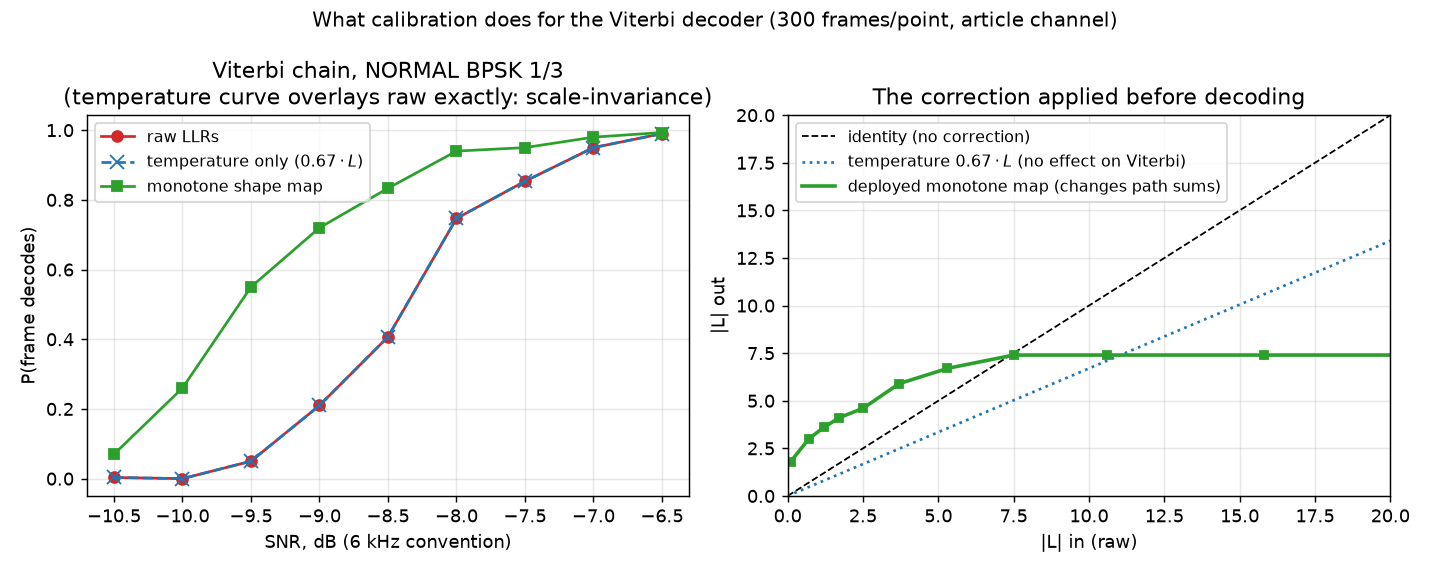
\includegraphics[width=\textwidth]{images/viterbi_recal.png}
    \caption{Calibration and the Viterbi decoder (reproduce with
             \texttt{experiments/viterbi\_recal.py}; parameters and
             per-point counts in
             \texttt{results/viterbi\_recal.json}).  Left: decode
             probability versus SNR for the same received frames
             decoded from raw LLRs, temperature-scaled LLRs
             ($0.67 \cdot L$ --- overlays raw exactly), and
             shape-mapped LLRs.  Right: the deployed monotone map
             against the identity and the temperature line: it boosts
             weak LLRs above identity and caps the top at the
             data-justified $\approx 7.4$.}
    \label{fig:viterbi_recal}
\end{figure}

\subsection{Deployment}

Alongside the static map, a per-frame temperature
$\alpha = 2\,\mathbb{E}[Lx]/\mathrm{Var}[Lx]$ is fitted from the 96
known bits of each decoded header (a Gaussian-consistency fit), which
keeps LLR scales consistent across frames --- a prerequisite for the
HARQ combining of Section~\ref{sec:coding}.  Following the
faithful-defaults principle, recalibration is \textbf{off} in the plain
\texttt{Transceiver} and enabled by the link-layer station
(\texttt{llr\_recal="auto"}).  The entire rate ladder was re-measured
with recalibration enabled; Section~\ref{sec:link} carries the
resulting sensitivities (mid-ladder BPSK/QPSK rungs gained
0.7--1.4\,dB).

\input{sections/07-coding-extensions}
\section{Link Layer}
\label{sec:link}

Two half-duplex stations form \emph{two directed links}, each governed
by its receiver --- only the receiver knows its own noise floor.  There
is no shared ``link mode'' to negotiate; each side requests what it can
hear.

\subsection{The Rate Ladder}

Thirteen operating points (mode $\times$ modulation $\times$ code
rate, dominated rungs removed) span \textbf{7.8--1059\,bit/s} over
\textbf{$-17.9\ldots+4.7$\,dB} (Table~\ref{tab:ladder}).  Every
sensitivity is measured, not derived
(\texttt{experiments/ladder\_sweep.py}, 48 packets/point, recalibrated
receiver; full PER curves in \texttt{results/ladder\_recal.json}).
Requests and grants are ladder indices carried in the link-control
word.  One quirk is documented: rung 1 (ROBUST BPSK 1/3) is dominated
by rung 2 (faster, equally sensitive) and is kept only for
ladder-index stability --- it is never selected.

\begin{table}[H]
    \centering
    \caption{The measured rate ladder (PER $\le 10\,\%$ sensitivities,
             recalibrated receiver, 6\,kHz-band SNR).}
    \label{tab:ladder}
    \small
    \begin{tabular}{@{}rlrr@{\hspace{2em}}rlrr@{}}
    \toprule
    \# & \textbf{mode/mod/FEC} & \textbf{bit/s} & \textbf{dB} &
    \# & \textbf{mode/mod/FEC} & \textbf{bit/s} & \textbf{dB} \\
    \midrule
    0 & EXTREME BPSK 1/3 & 7.8 & $-17.9$ & 7  & NORMAL QPSK 1/2  & 353  & $-5.3$ \\
    1 & ROBUST BPSK 1/3  & 31  & $-11.7$ & 8  & NORMAL QPSK 2/3  & 471  & $-3.8$ \\
    2 & ROBUST BPSK 1/2  & 46  & $-11.8$ & 9  & NORMAL QPSK 3/4  & 529  & $-2.2$ \\
    3 & ROBUST QPSK 1/3  & 62  & $-11.3$ & 10 & NORMAL QAM16 1/2 & 706  & $+0.7$ \\
    4 & NORMAL BPSK 1/3  & 118 & $-7.6$  & 11 & NORMAL QAM16 2/3 & 941  & $+2.6$ \\
    5 & NORMAL BPSK 1/2  & 176 & $-7.3$  & 12 & NORMAL QAM16 3/4 & 1059 & $+4.7$ \\
    6 & NORMAL QPSK 1/3  & 235 & $-7.0$  &    &                  &      &         \\
    \bottomrule
    \end{tabular}
\end{table}

\subsection{The Link-Control Word}

Every frame --- data, ACKs, everything --- piggybacks a 20-bit word in
\texttt{Data.reserved}:
\texttt{seq(2)\,|\,ack(2)\,|\,req\_rung(4)\,|\,snr\_report(4)\,|\,%
freq\_corr(5)\,|\,flags(3)}.  The SNR report uses 2\,dB steps; the
frequency-correction field carries $\pm 120$\,Hz in 8\,Hz steps
(Section~\ref{sec:afc}); flags are last-fragment, no-data (ACK-only),
and priority-stream.

\subsection{Rate Adaptation: Three Feedback Paths}

Figure~\ref{fig:adaptation} shows the controller.  On the receive
side, per-frame SNR estimates pass through a fade-aware filter (the
second-lowest of recent measurements, age-windowed to 60\,s) before
driving the rung request: upshift requires the target rung's
sensitivity plus 2.5\,dB of held margin, downshift triggers below
1\,dB (the hysteresis band prevents ping-pong), and inbound
\emph{silence} decays the request and purges the measurement history
--- without the purge, stale pre-fade measurements resurrect a high
rung the moment one frame gets through.

\begin{figure}[H]
    \centering
    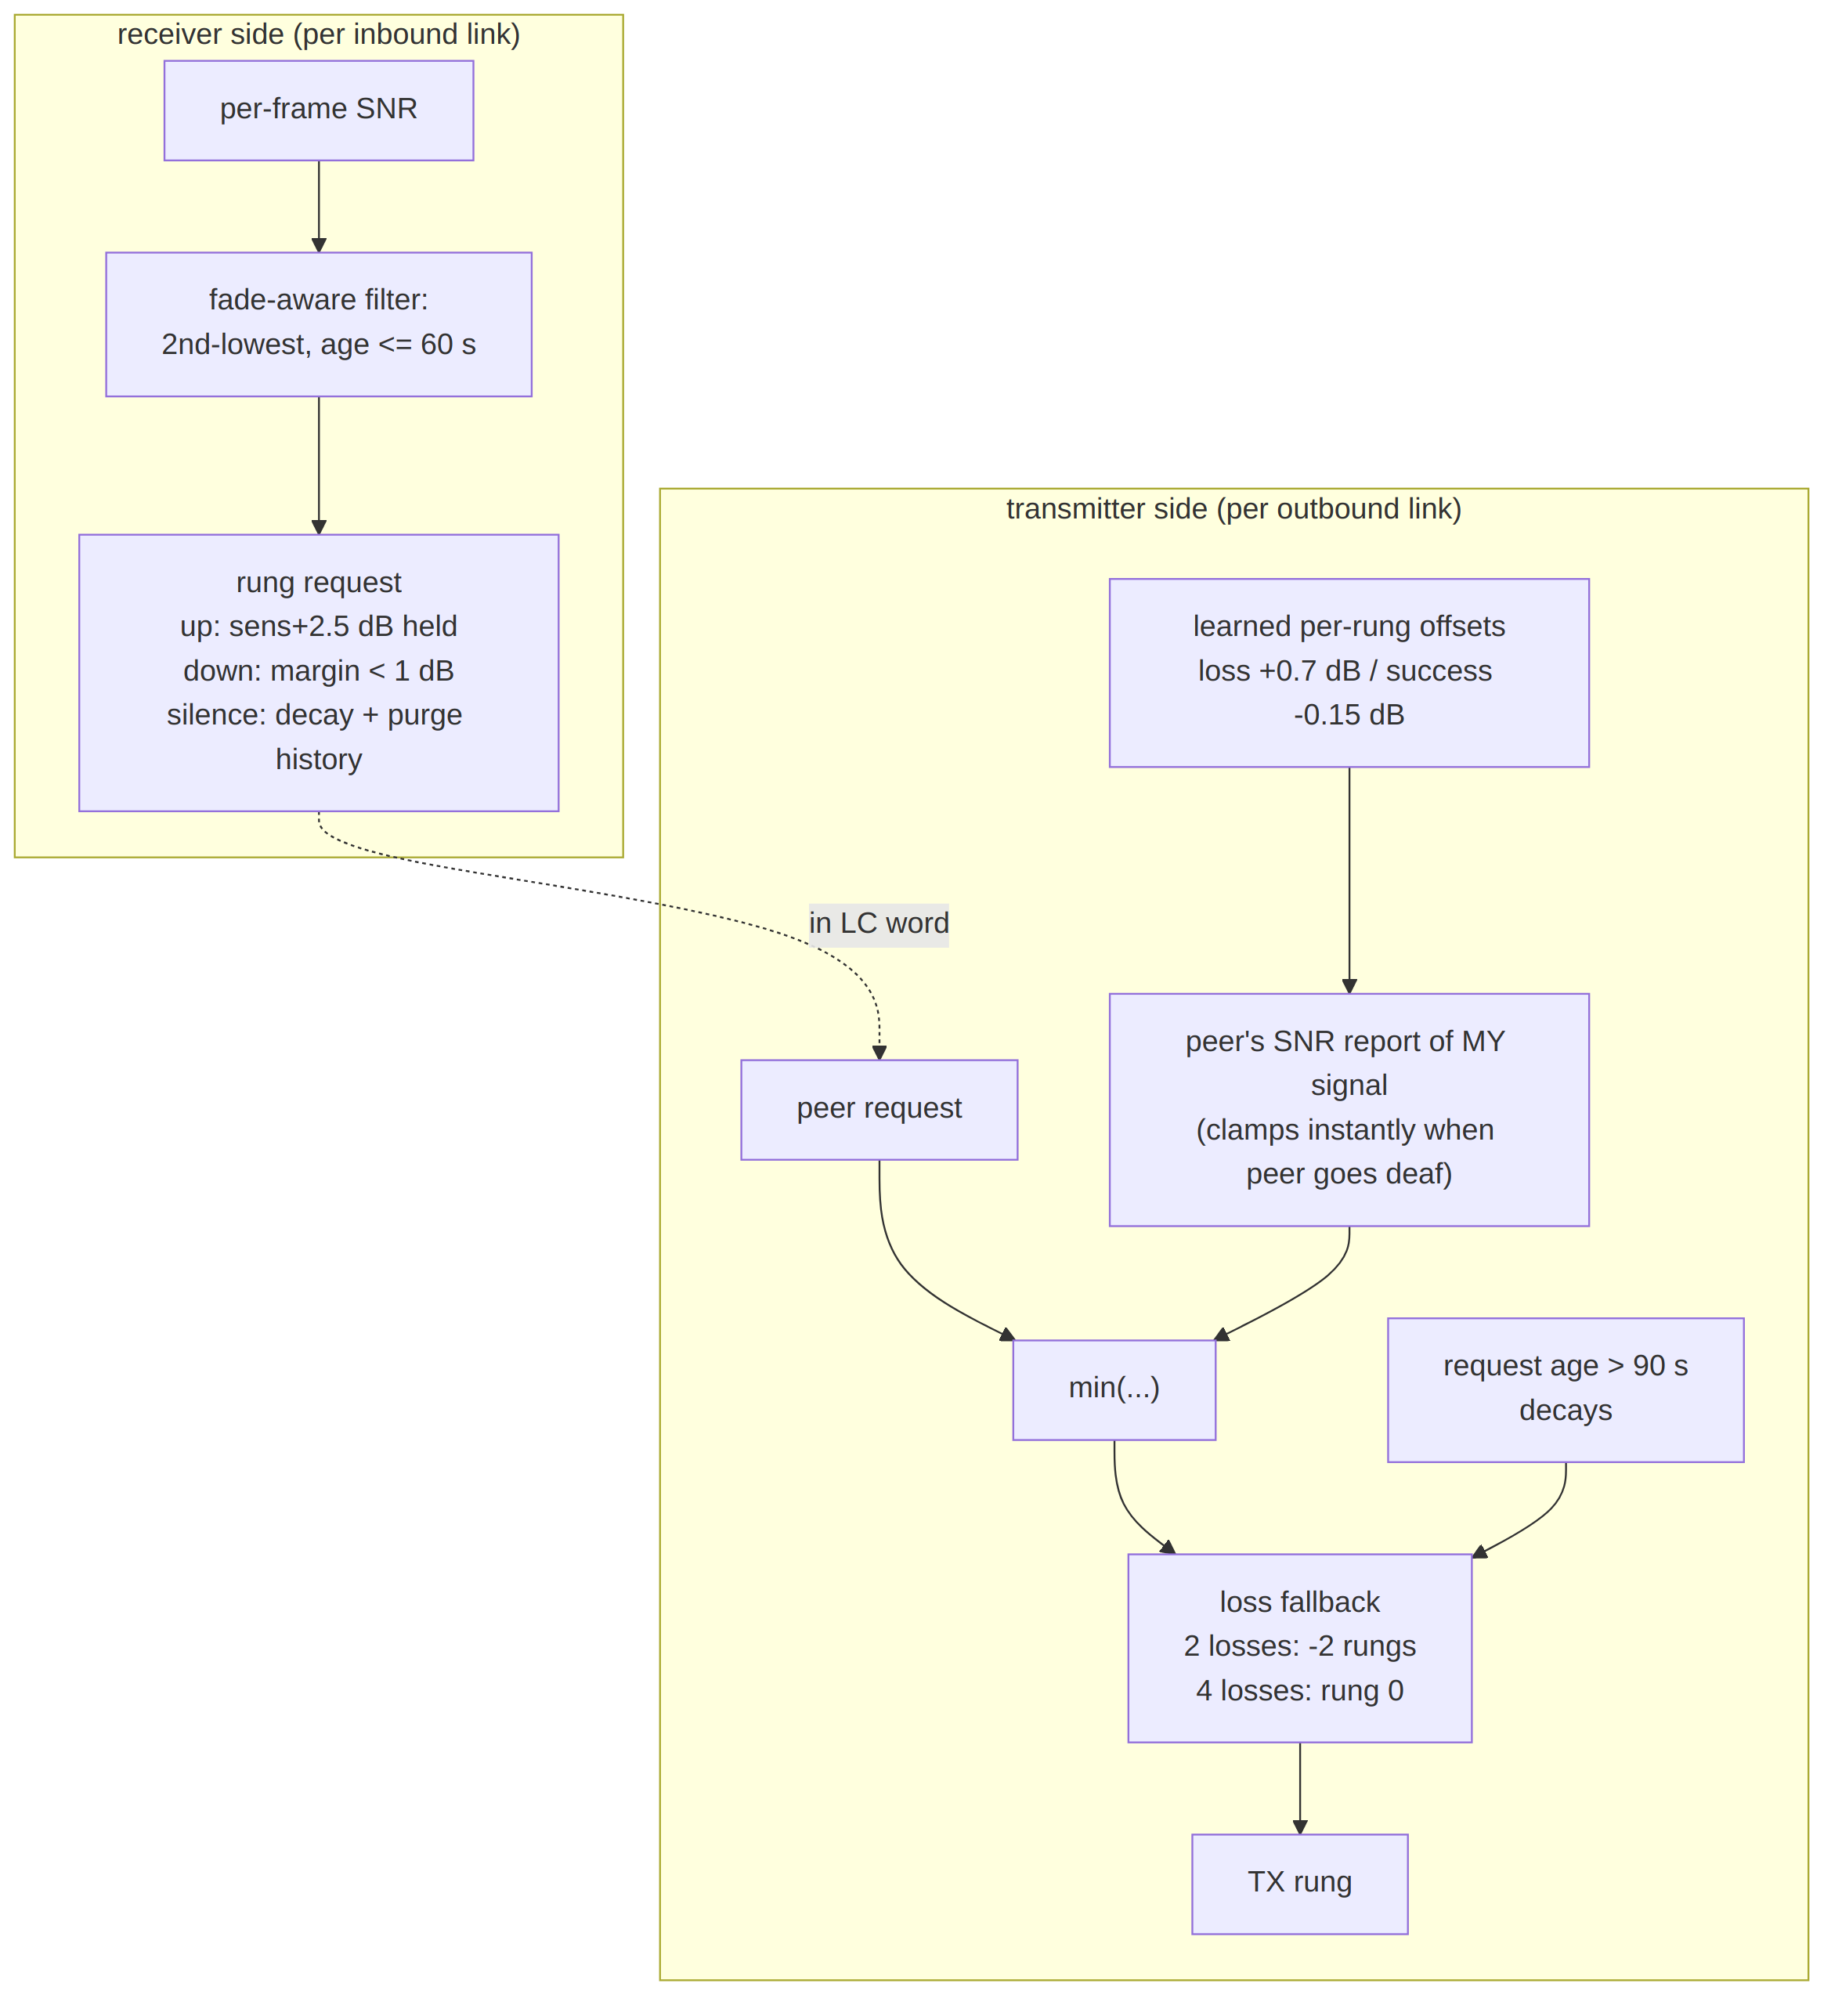
\includegraphics[width=\textwidth]{images/adaptation.png}
    \caption{Receiver-driven rate adaptation.  The three feedback paths
             have three different latencies: the peer's explicit
             request (one round trip), the peer's SNR report of
             \emph{your} signal (instant clamp when the peer goes
             deaf), and loss-driven fallback (no feedback at all).}
    \label{fig:adaptation}
\end{figure}

On the transmit side, the rung is the minimum of the peer's request
and a cap derived from the peer's SNR report of our own signal,
adjusted by \emph{learned per-rung offsets} ($+0.7$\,dB on loss,
$-0.15$\,dB on success --- correcting the static table per
deployment), with loss fallback (2 consecutive losses
$\rightarrow -2$ rungs, 4 $\rightarrow$ rung 0) and staleness decay.
Bootstrap is trivial by construction: both sides start at rung 0
(EXTREME), which works whenever anything works, and one decoded
exchange carries enough measurement to jump directly to the
SNR-indicated rung.

\subsection{ARQ, QoS, and Preemption}

ARQ is stop-and-wait with piggybacked ACKs (the 2-bit sequence number
suffices), enhanced by the HARQ combining of Section~\ref{sec:coding}.
An invariant worth recording: sequence numbers 0--7 are all
legitimate, so ``nothing received yet'' is represented by
\texttt{None}, never a magic value --- the initial implementation used
7 as a sentinel and deadlocked the moment a real frame carried
sequence 7.

QoS is policy, not machinery: three classes (control $>$ interactive
$>$ bulk) with strict priority; per-class air-time caps size fragments
(a 27-byte EXTREME frame is 43\,s of air time, so latency budgeting
happens at segmentation); control and ACK traffic rides one rung below
bulk for extra margin.  The priority stream \emph{preempts} an
in-progress bulk message at fragment boundaries --- the
priority-stream LC flag selects one of two reassembly buffers --- so
an urgent message injected mid-transfer arrives $\sim$23\,s before the
bulk completes instead of after it.

\subsection{Burst Windows and Streaming}
\label{sec:burstwin}

Bulk transfers use selective repeat: a window of fragments goes out
back-to-back, answered by one bitmap acknowledgment
(NACK-by-omission).  Where the PHY offers streaming
(Section~\ref{sec:stream}), the whole window is sent behind a
\emph{single} preamble and header rather than one preamble per
fragment.  The packets are byte-identical to per-frame burst fragments
--- one spare bit in the sub-header's index byte marks a fragment as
streamed --- so a receiver without streaming support still decodes the
first block of every burst as an ordinary fragment.  That property is
what makes the fallback safe rather than fatal.

The window is chosen once, at engage, as
$\min(\text{operator ceiling}, \text{buffer cap},
\text{fragment count})$, then clipped by an air-time cap so that a
single transmission can never outlast a plausible fade --- everything
in a streamed window is exposed before any of it is acknowledged.
Sizing the window to the transfer is what makes a short transfer cost
exactly one acknowledgment, which is the deferred-NAK arrangement of
LTP and CFDP arrived at through a constant rather than new wire
format.  Measured on a 14\,kB file over the virtual channel: window 4
takes 14 transmissions, window 8 takes 9, window 16 takes 6.

Resizing the window \emph{during} a transfer was implemented and then
reverted on the evidence.  Halving it on each streamed-window timeout,
rather than striking out of streaming, collapsed the window
$16\to8\to4\to2\to1$ with no path back --- it grows only on a fully
acknowledged window, which never happens inside a fade --- and produced
196 transmissions with 72 timeouts against 134 and 9 for the
strike-out path.  On a clean channel the two were indistinguishable.
When a fade is what breaks a burst, the correct response is to stop
streaming, not to stream less.

Three conditions end streaming for a transfer, and they are not the
same kind of statement.  A bitmap that acknowledges at most one
fragment of a window of three or more is the signature of a peer
decoding only the first block: that is a statement about the
\emph{peer}, and it is remembered across transfers, because a receiver
unable to follow a stream will not learn to between them.  Repeated
timeouts and a transmitter-side build refusal describe the
\emph{channel} and the local buffers respectively, and deliberately do
not stick --- a fading channel raises timeouts against a peer that
streams perfectly well, and making that sticky would disable streaming
for the session on a capable link.  The peer verdict is not permanent
either, since a deep fade can forge the one-fragment signature:
streaming is probed again after eight transfers, which bounds a wrong
verdict to one wasted window per retry period while a genuinely
incapable peer costs two windows per period instead of two per
transfer.

\subsection{The Reply Timer}
\label{sec:rto}

A station that has transmitted and expects an answer must decide how
long to wait.  The budget splits along what is knowable.  The reply's
\emph{air time} is computable exactly from the rung and the expected
reply length, and it swings by a factor of forty across the ladder, so
smoothing it would be meaningless.  Everything else --- the peer's
turnaround, its decode time, its wait for the channel to clear, its
scheduling, and the error in our guess of which rung it will answer at
--- is latency that can only be measured.

The air term is therefore computed and the overhead is estimated in
the manner of RFC~6298: a smoothed mean and variance
($\alpha = 1/8$, $\beta = 1/4$) with the budget set at
$\text{srtt} + 4\,\text{rttvar}$.  Karn's rule keeps ambiguous
exchanges out of the estimator --- a reply that follows a
retransmission cannot be attributed to a particular transmission ---
and a timeout doubles the timer until a clean exchange clears the
backoff.  Against a peer that consistently takes 0.40\,s, the
2.30\,s bootstrap guess converges to 0.40\,s.

This replaces a fixed margin that had already caused a
misdiagnosis. When the host could not sustain the demonstration
harness's 25$\times$ time compression, the two stations' sample-derived
clocks drifted apart --- the mostly-transmitting station stayed
current while the one decoding three receivers fell behind --- and the
transmitter timed out before the receiver had finished the burst in
its own timeline.  Every timeout landed on one station and none on the
other, with the reply arriving immediately after each: a signature
that reads exactly like a protocol failure and is not one.

\subsection{Simplex Channel Access}

Both stations share one frequency and are deaf while transmitting.
Figure~\ref{fig:simplex} shows the access state machine.  The
load-bearing rules: carrier sense before keying; the listen window is
sized from the \emph{expected reply's} air time at the peer's rung; a
timeout on a \emph{busy} channel is not a loss (the peer may be
replying at a slower rung); random 1--6\,s backoff breaks the symmetry
of two stations keying together; and a station replies only to frames
that carried data --- no ACK-of-ACK loops.

\begin{figure}[H]
    \centering
    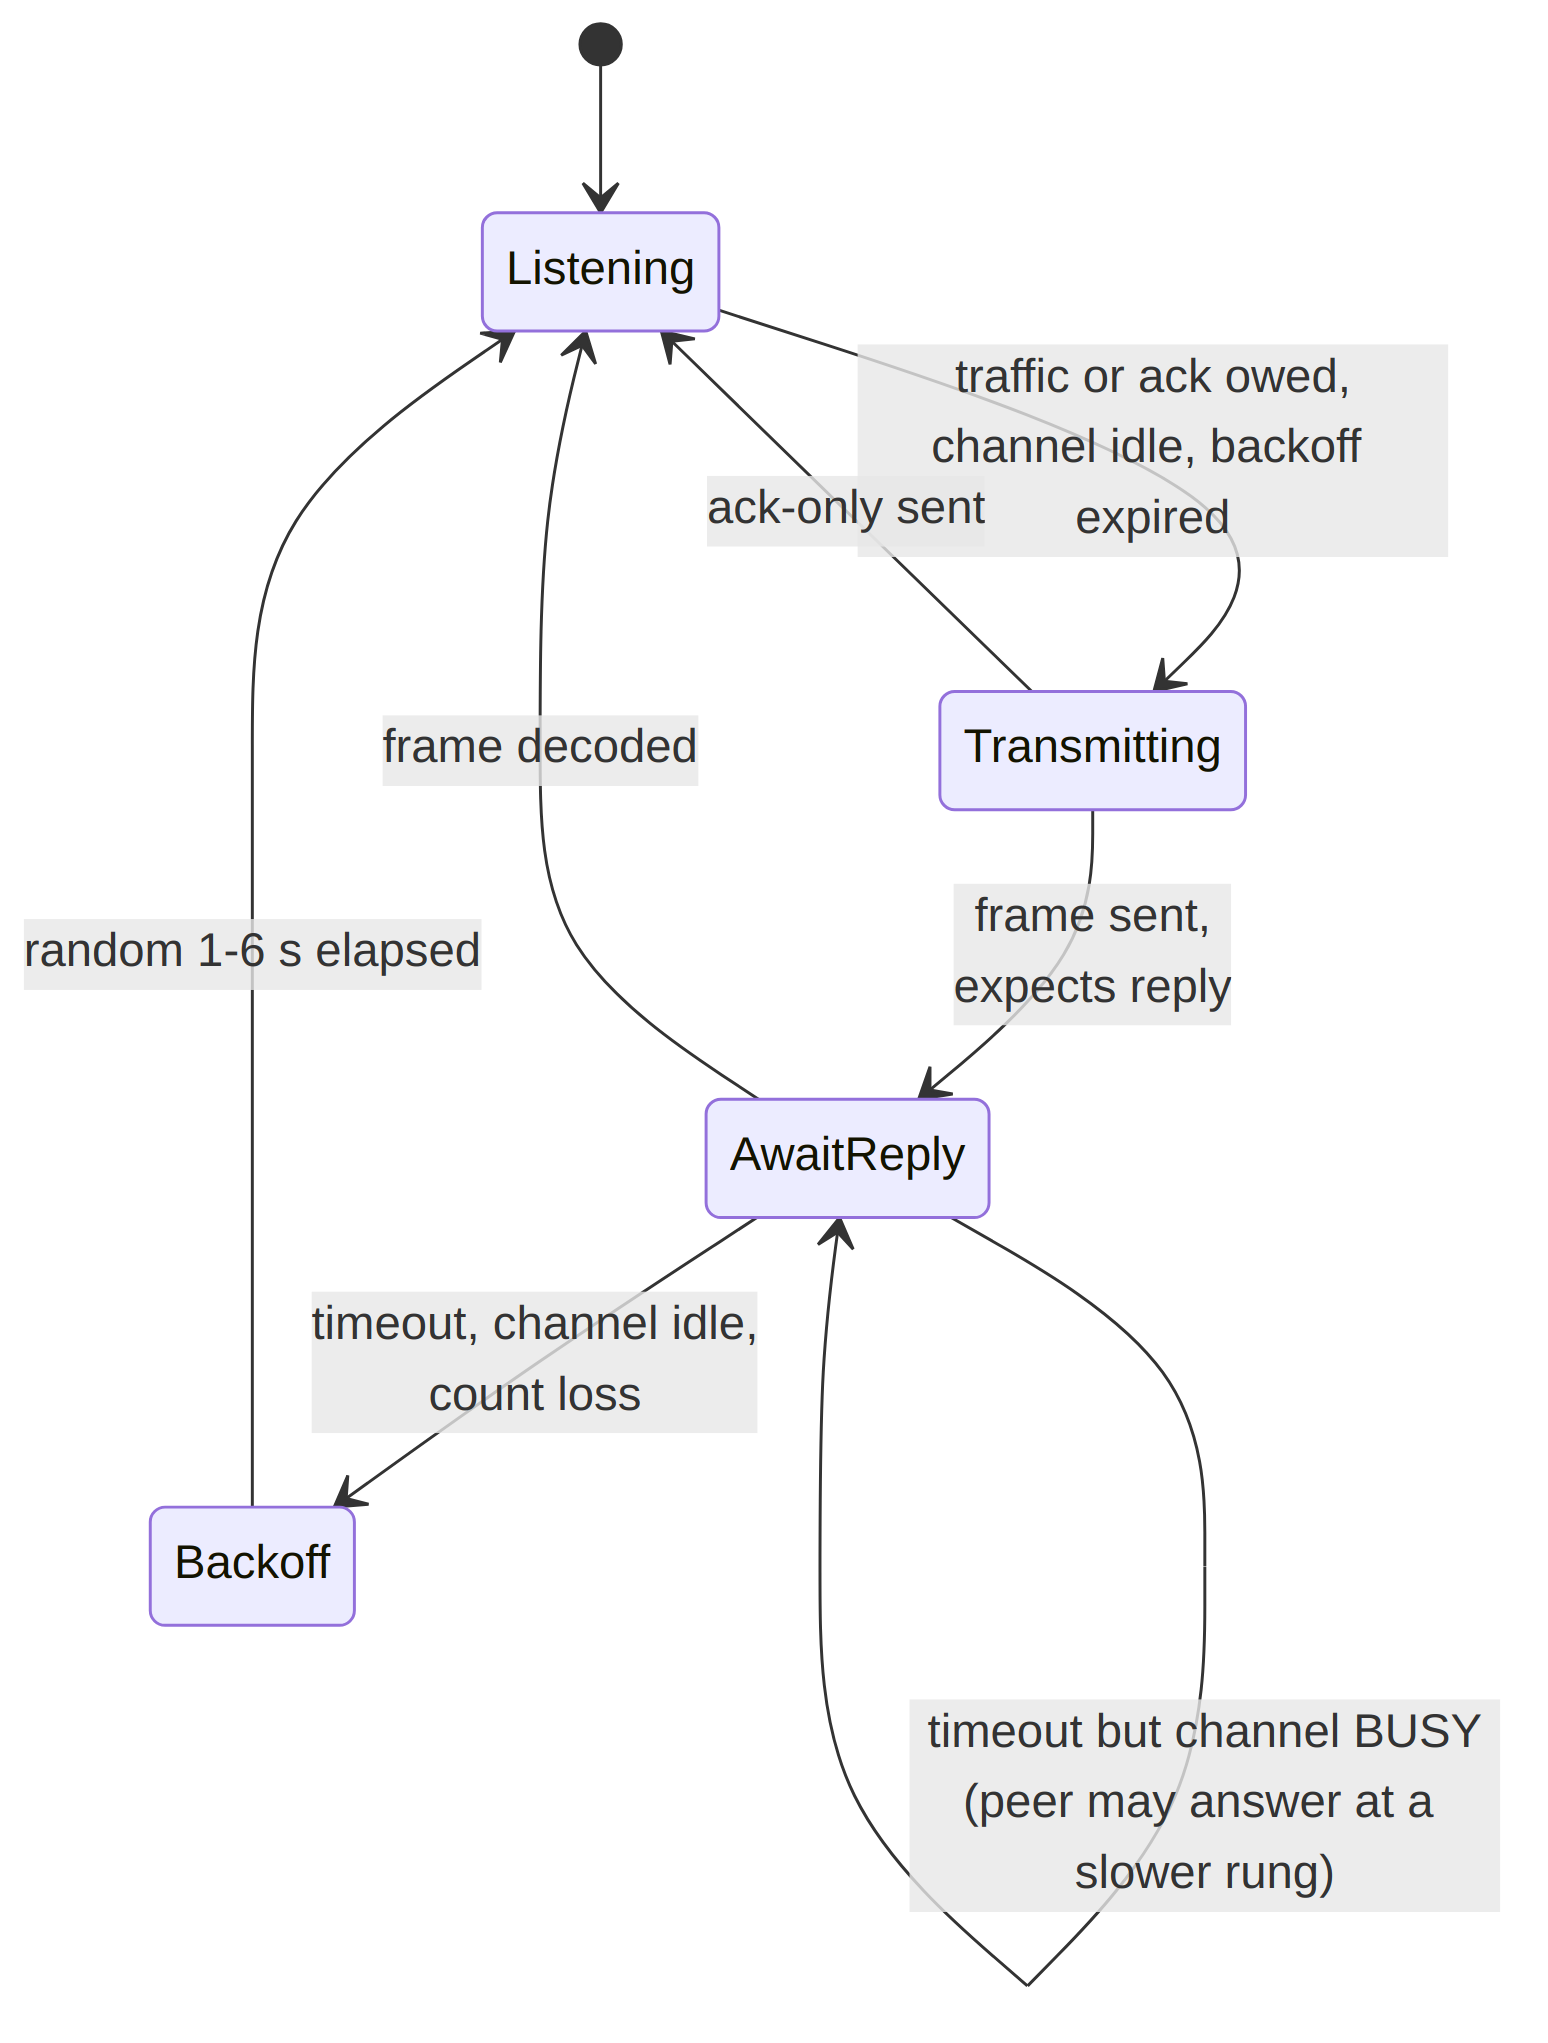
\includegraphics[width=0.85\textwidth]{images/simplex_state.png}
    \caption{Simplex channel-access state machine
             (\texttt{LinkStation.poll\_tx}).}
    \label{fig:simplex}
\end{figure}

The whole-system test (\texttt{experiments/simplex\_session.py}) runs
two stations with bidirectional QoS traffic and a $-14$\,dB fade in
the middle of the bulk transfer: all messages deliver bit-exact in QoS
priority order, the fade costs four timeouts and one
fallback-and-recover cycle, and the session terminates without
deadlock at 11--22\,bit/s effective on the shared channel.
Figure~\ref{fig:link_adaptation} shows the controller-level
simulation: bootstrap at EXTREME, a fast climb to the QPSK rungs,
loss-driven fallback within two frames of a sudden fade, and
recovery.

\begin{figure}[H]
    \centering
    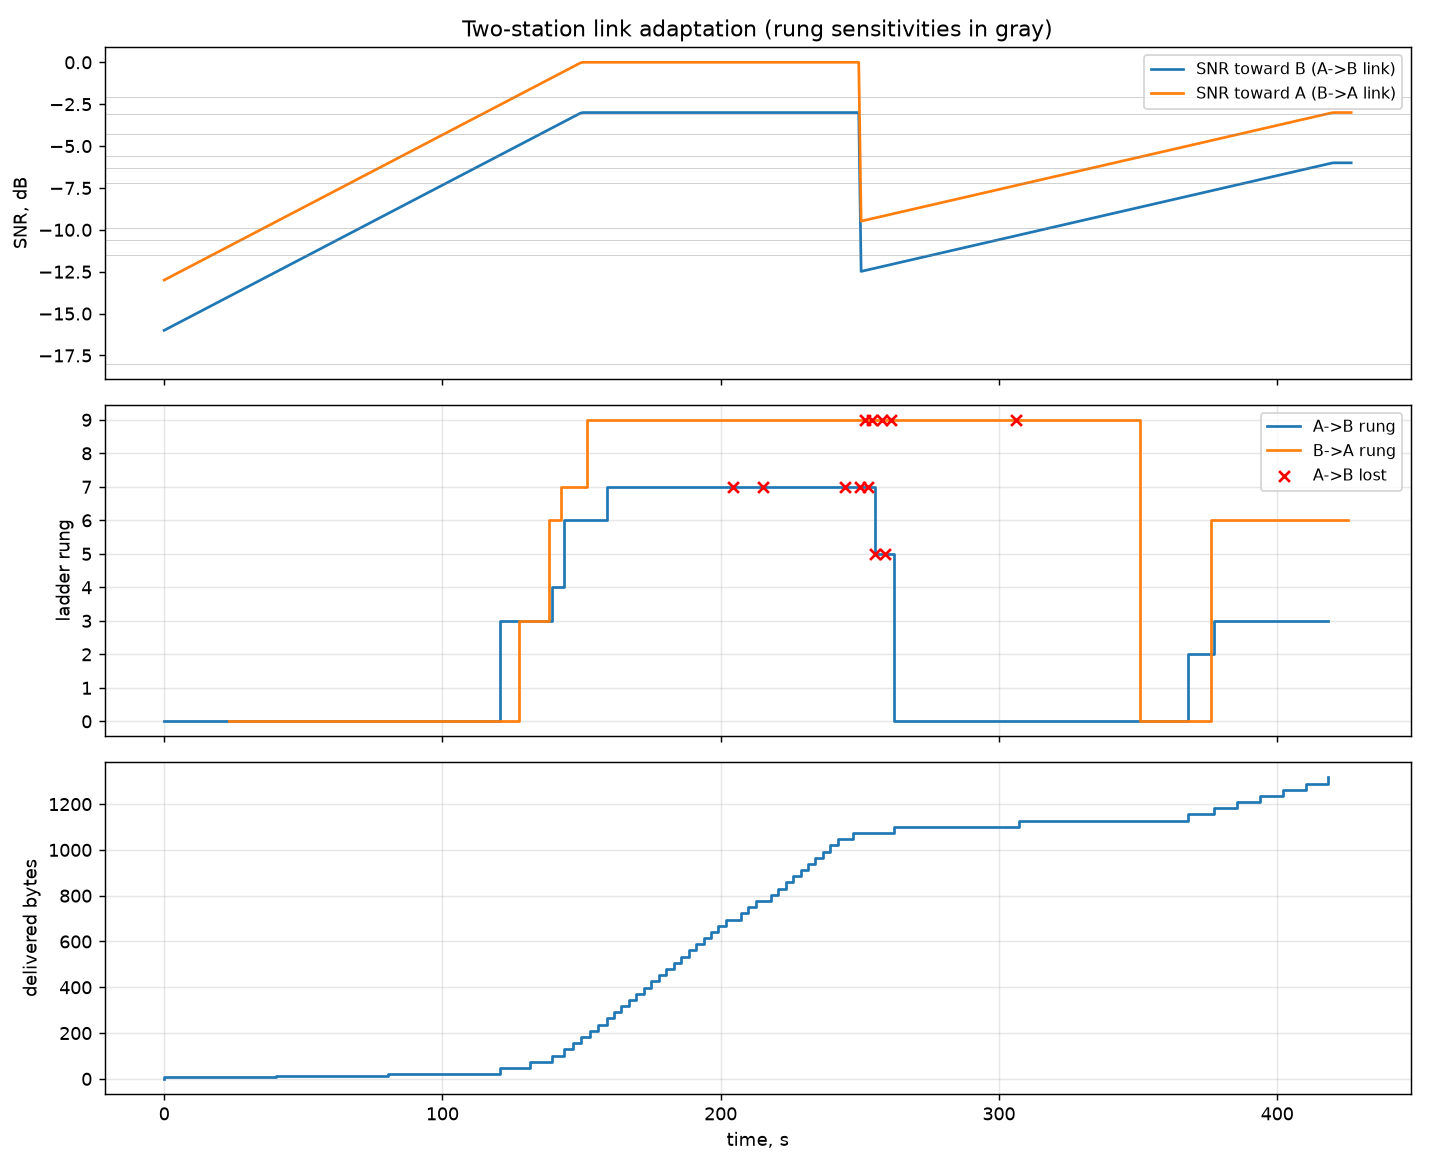
\includegraphics[width=\textwidth]{images/link_adaptation.png}
    \caption{Controller-level two-station simulation
             (\texttt{experiments/link\_adaptation.py}): asymmetric
             channel, $-16$\,dB start, sudden fade; 1290/1500 bytes
             delivered at 24\,bit/s effective goodput including ACK
             overhead and turnarounds.}
    \label{fig:link_adaptation}
\end{figure}

\section{AFC Frequency Netting}
\label{sec:afc}

The receiver measures the peer's carrier offset on every decoded frame
anyway (\texttt{stats.cfo\_hz}), so the link closes the loop: the
5-bit LC field carries ``shift your carrier by $-X$\,Hz'' requests
($\pm 120$\,Hz per frame, 8\,Hz steps, $\pm 12$\,Hz deadband), and the
peer trims its \emph{shared} reference oscillator.  Trimming the
shared reference moves TX and RX together --- which is exactly why
asking the peer to correct beats retuning locally
(Section~\ref{sec:rf}).  Corrections are applied at \textbf{half
gain}: both sides act on measurements that are one frame stale, and
full-gain corrections would swap the offset between the stations each
turn instead of converging (Figure~\ref{fig:afc}).

\begin{figure}[H]
    \centering
    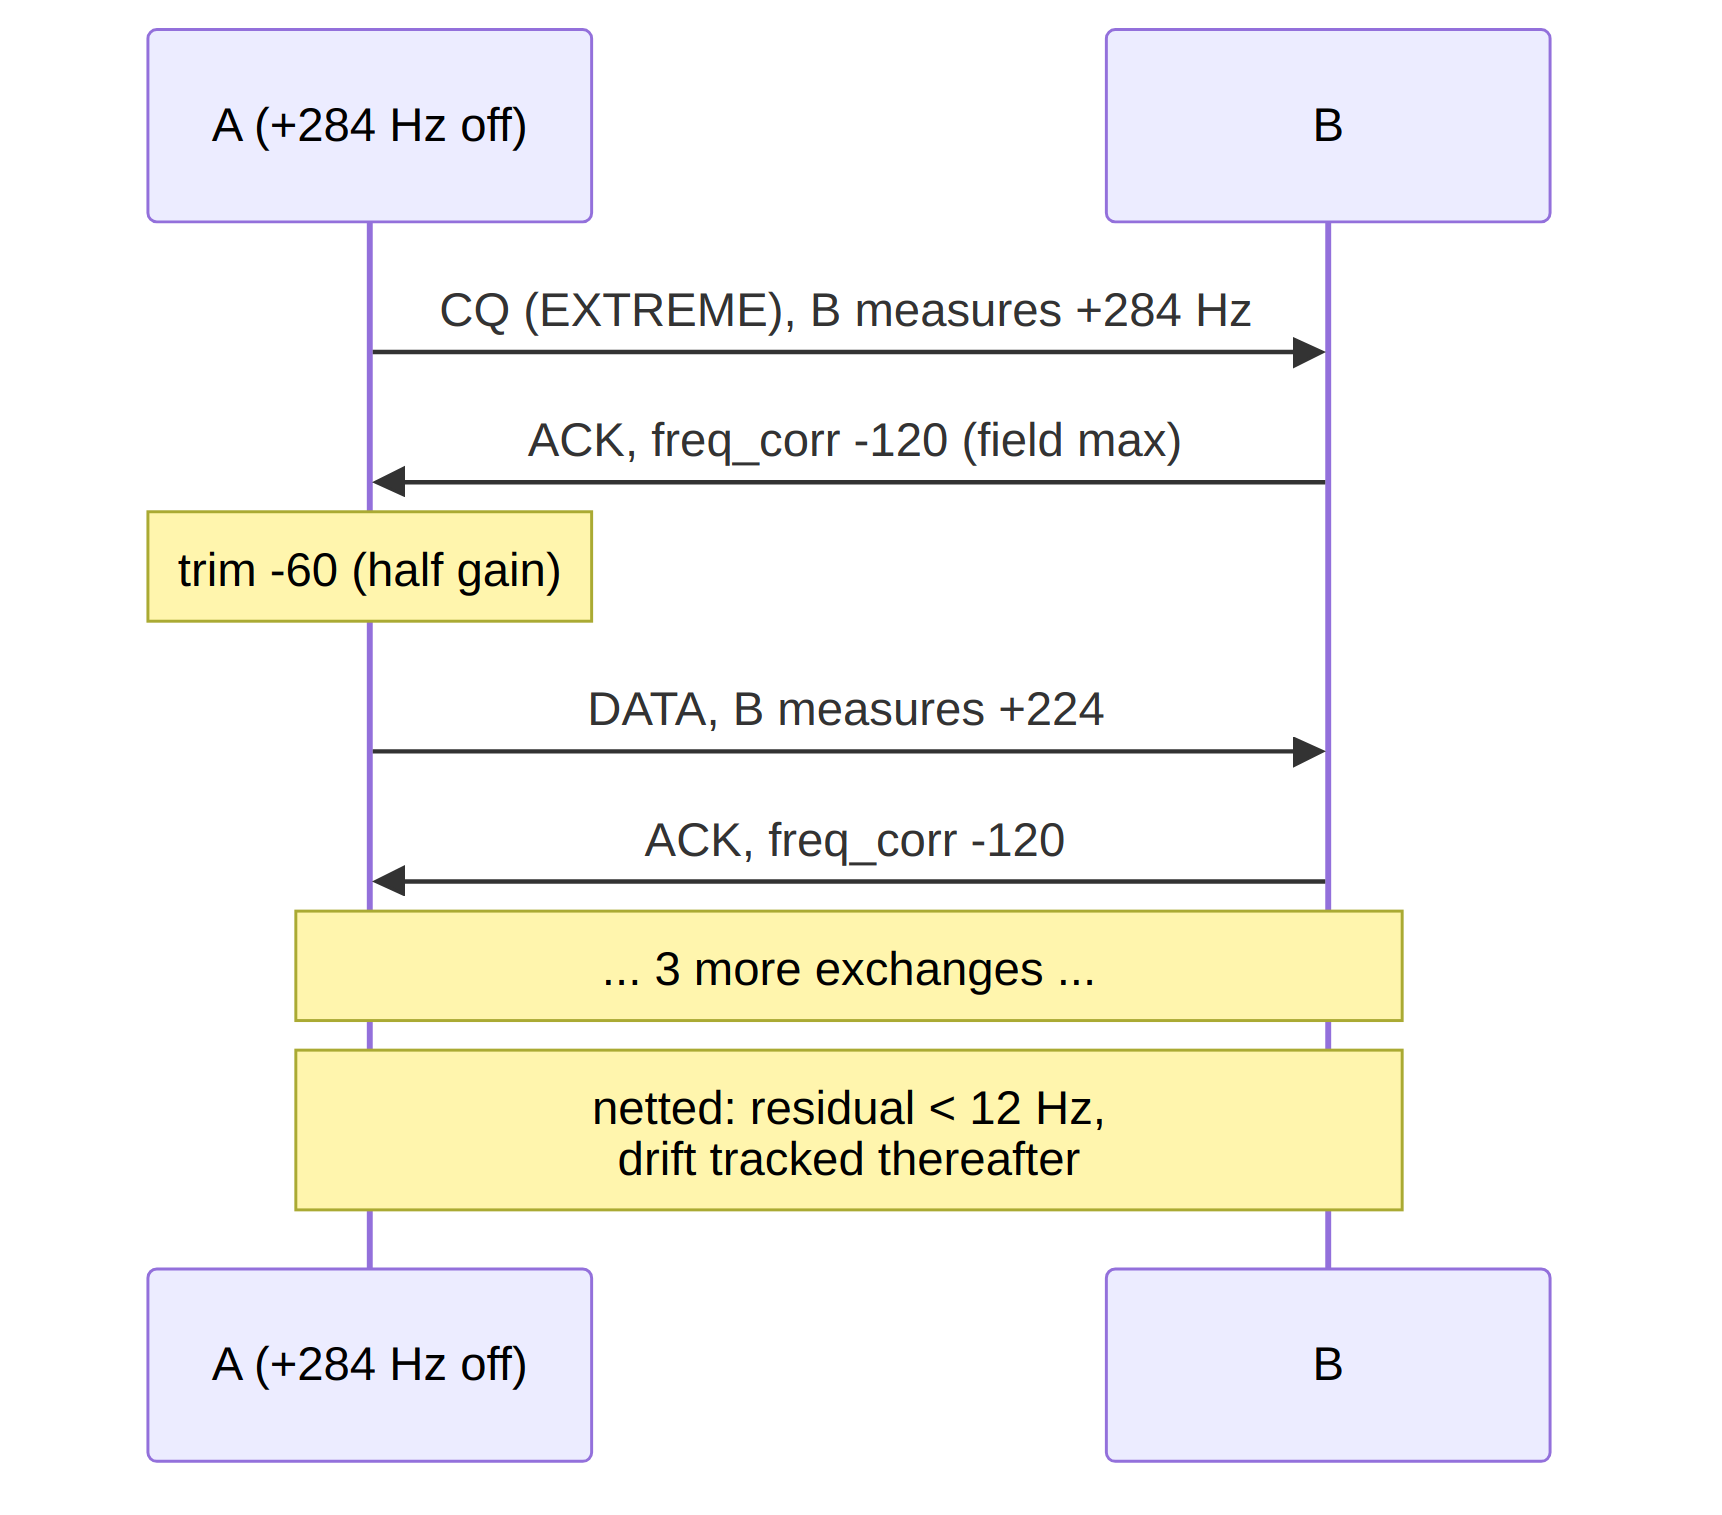
\includegraphics[width=0.85\textwidth]{images/afc_seq.png}
    \caption{AFC netting from a $+284$\,Hz initial offset.}
    \label{fig:afc}
\end{figure}

\subsection{Guard Rails}

The loop observes only the \emph{differential} offset, so without
bounds the pair's common frequency random-walks over a long session
--- out of the channel slot, into bystanders' passbands, or off the
rig's trim range.  Two mechanisms bound it:

\begin{itemize}
    \item \texttt{afc\_max\_trim\_hz} (default $\pm 150$\,Hz)
          hard-clamps each station's \emph{cumulative} trim.  Requests
          beyond the budget are partially honoured or refused, the
          peer's own headroom carries the rest, and any residual is
          left to the modem's $\pm 300$\,Hz CFO tolerance --- the link
          keeps working, just without full netting.
    \item \texttt{afc\_anchor=True} designates a station (e.g.\ the CQ
          caller) that never trims, pinning the absolute frequency
          entirely; the peer does all the correcting.
\end{itemize}

\subsection{Measured Behaviour}

\texttt{experiments/afc\_netting.py} runs two worn-TCXO rigs on
14.2\,MHz starting \textbf{$+284$\,Hz apart} (near the modem's
$\pm 375$\,Hz limit) with opposing thermal drifts: netted to within
the deadband in $\approx$5 correction exchanges ($\approx$104\,s ---
EXTREME bootstrap frames dominate the wall clock), steady-state
$|$CFO$| \le 11$\,Hz under continuing 0.09\,Hz/s relative drift,
400/400 bytes delivered.  The guard scenarios behave as designed:
default budgets net fully (final $|$CFO$|$ 3\,Hz, trims clamped at
$-150/+144$\,Hz); deliberately tight $\pm 40$\,Hz budgets stop at
their limits leaving a 222\,Hz residual \emph{by design}, with the
link still delivering on CFO tolerance alone; an anchored station A
forces B to absorb the full $+292$\,Hz and the pair's absolute
frequency never moves.  Beyond robustness margin, a netted link could
shrink EXTREME's per-symbol frequency-search range (compute) and eases
mask-grid detection at the extremes.

\section{RF Layer and Channel Models}
\label{sec:rf}

Two channel models coexist.  The audio-domain simulator
(\texttt{channel.py}) is the article's model --- timing offset, CFO
with quadratic drift, optional Rayleigh fading, multipath
$[1,0,0.4,0,0,0.2]$, AWGN, BSC block flips ($p=10^{-3}$) and BEC block
erasures ($p=2\cdot 10^{-2}$) --- and drives most sweeps.  The RF
layer (\texttt{rf.py}) models the actual transceiver chain, so carrier
offsets \emph{emerge from oscillator physics} instead of being
injected as parameters.

\subsection{The SSB Chain}

Simulation runs at a 48\,kHz IF rate with a 12\,kHz carrier standing in
for the RF carrier; LO errors are specified in ppm of the nominal RF
frequency (e.g.\ 7.1\,MHz), so audio-band offsets come out physically
correct (Figure~\ref{fig:rf_chain}).

\begin{figure}[H]
    \centering
    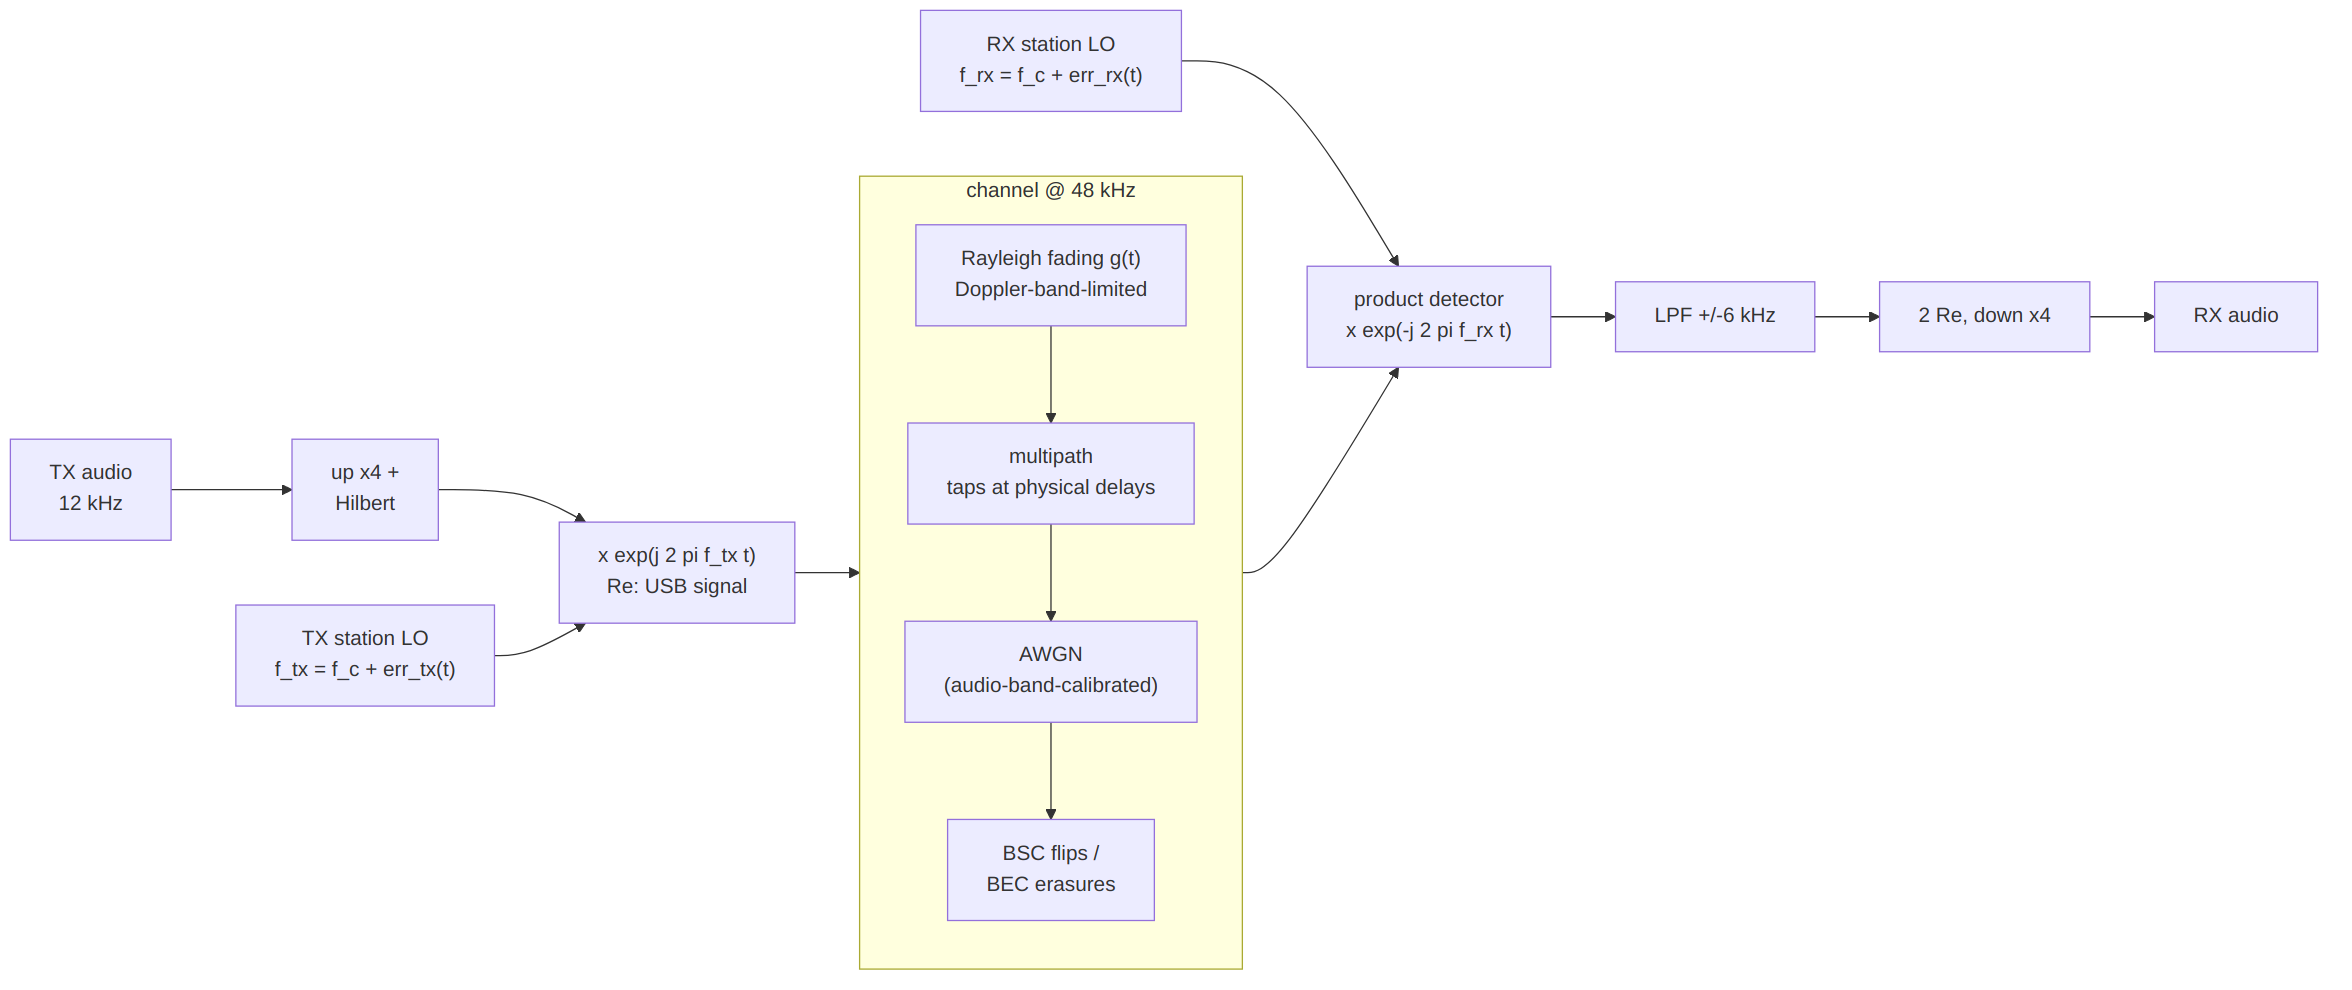
\includegraphics[width=\textwidth]{images/rf_chain.png}
    \caption{The RF chain: USB modulator, 48\,kHz channel (fading,
             multipath, AWGN, BSC/BEC), product detector.}
    \label{fig:rf_chain}
\end{figure}

\subsection{The LO Model}

Each \texttt{StationRF} has \emph{one} reference oscillator shared by
its TX and RX, as in a real transceiver:
\[
    \mathrm{err}(t) \;=\; f_{\mathrm{rf}} \cdot \mathrm{ppm} \cdot
    10^{-6} \;+\; \mathrm{drift}_{\mathrm{Hz/s}} \cdot t \;+\;
    \mathrm{trim}_{\mathrm{Hz}},
\]
and the audio CFO between two stations is
$\mathrm{err}_{tx}(t) - \mathrm{err}_{rx}(t)$
(Figure~\ref{fig:lo_model}).  Validated against the modem's own CFO
measurements to 0.1\,Hz at $+99.4$, $-106.5$, and $+284.0$\,Hz
scenarios.  \texttt{trim\_hz} is the AFC hook of
Section~\ref{sec:afc}.

\begin{figure}[H]
    \centering
    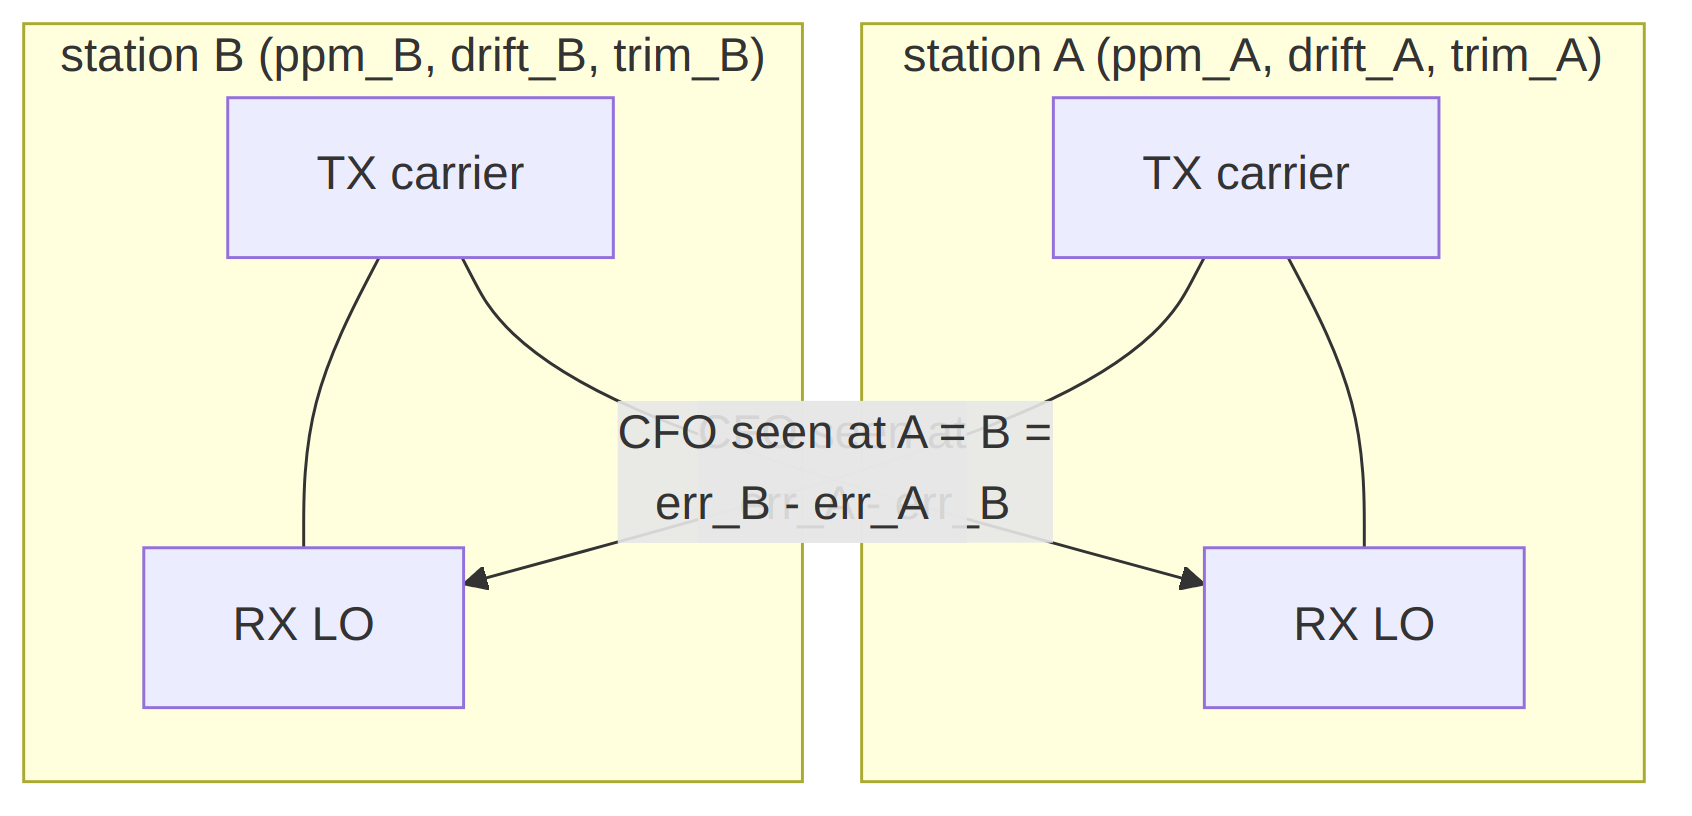
\includegraphics[width=0.75\textwidth]{images/lo_model.png}
    \caption{Per-station shared-reference LO model: where CFO comes
             from.}
    \label{fig:lo_model}
\end{figure}

\subsection{Calibration Subtleties}

Three traps are documented in code comments because each silently
costs dB if gotten wrong:

\begin{itemize}
    \item \textbf{AWGN sizing.}  The product detector's
          $\mathrm{Re}(\cdot)$ halves \emph{uncorrelated noise} power
          but not the coherent signal, so the RF noise variance factor
          is $2 \cdot P_{\mathrm{sig}} \cdot 10^{-\mathrm{SNR}/10}$
          --- not the naive bandwidth ratio, which is 3\,dB off.  With
          the correct factor the audio-band SNR convention matches the
          audio-domain simulator, so all measured sensitivities carry
          over (9/10 decodes at $-5$\,dB through the full RF chain).
    \item \textbf{Rayleigh fading.}  Complex Gaussian band-limited to
          the Doppler bandwidth (0.1--0.5\,Hz, typical HF QSB), unit
          mean power, applied to the analytic signal; AWGN is sized
          from the \emph{average} faded power, so instantaneous SNR
          swings around the nominal value.
    \item \textbf{Multipath at RF.}  The audio-domain tap delays are
          physical, so taps map to interpolation-factor-spaced
          positions at the RF rate.
\end{itemize}

\subsection{The Recorded Demonstration}

\texttt{experiments/demo\_wav.py} records a complete two-station
session through this chain: station A at $+6$\,ppm and B at $-8$\,ppm
on 7.1\,MHz (A$\rightarrow$B CFO $\approx +99.4$\,Hz, handled
invisibly by the protocol).  The output WAV is the audio of a
\emph{passive monitor} receiver with its own $+2$\,ppm LO --- A's
frames appear at $\approx +28$\,Hz and B's at $\approx -71$\,Hz in the
blind-decoded transcript (Appendix~\ref{app:demo}), per-station CFO
fingerprints with the thermal drift visible across the session.

\section{Fixed-Point RTL Reference Model}
\label{sec:fixed}

\texttt{ofdm\_phy/fixed/} is an integer-only twin of the modem,
structured the way an FPGA/ASIC datapath would be.  It is the golden
reference a future RTL implementation verifies against;
\texttt{experiments/fixed\_point.py} (24 checks,
Appendix~\ref{app:fixed}) cross-validates it against the float model
continuously.

\subsection{Receiver Datapath}

Figure~\ref{fig:fixed_rx} shows the complete integer receive path,
from int16 audio to decoded packet.  The model covers the \emph{full}
frame family: convolutional and LDPC FEC, BPSK/QPSK/16-QAM, all three
link modes, HARQ chase combining, and the optional calibrated-LLR
mode --- on the transmit side as well:
\texttt{build\_frame(fec="ldpc")} emits \texttt{ver=2} frames (the
LDPC accumulator encoding is already pure integer, so only the
header/codec switch was needed), and the Q15 constellations cover
BPSK, QPSK, and Gray 16-QAM (per-axis levels
$\{\pm 1, \pm 3\}/\sqrt{10}$).

\begin{figure}[H]
    \centering
    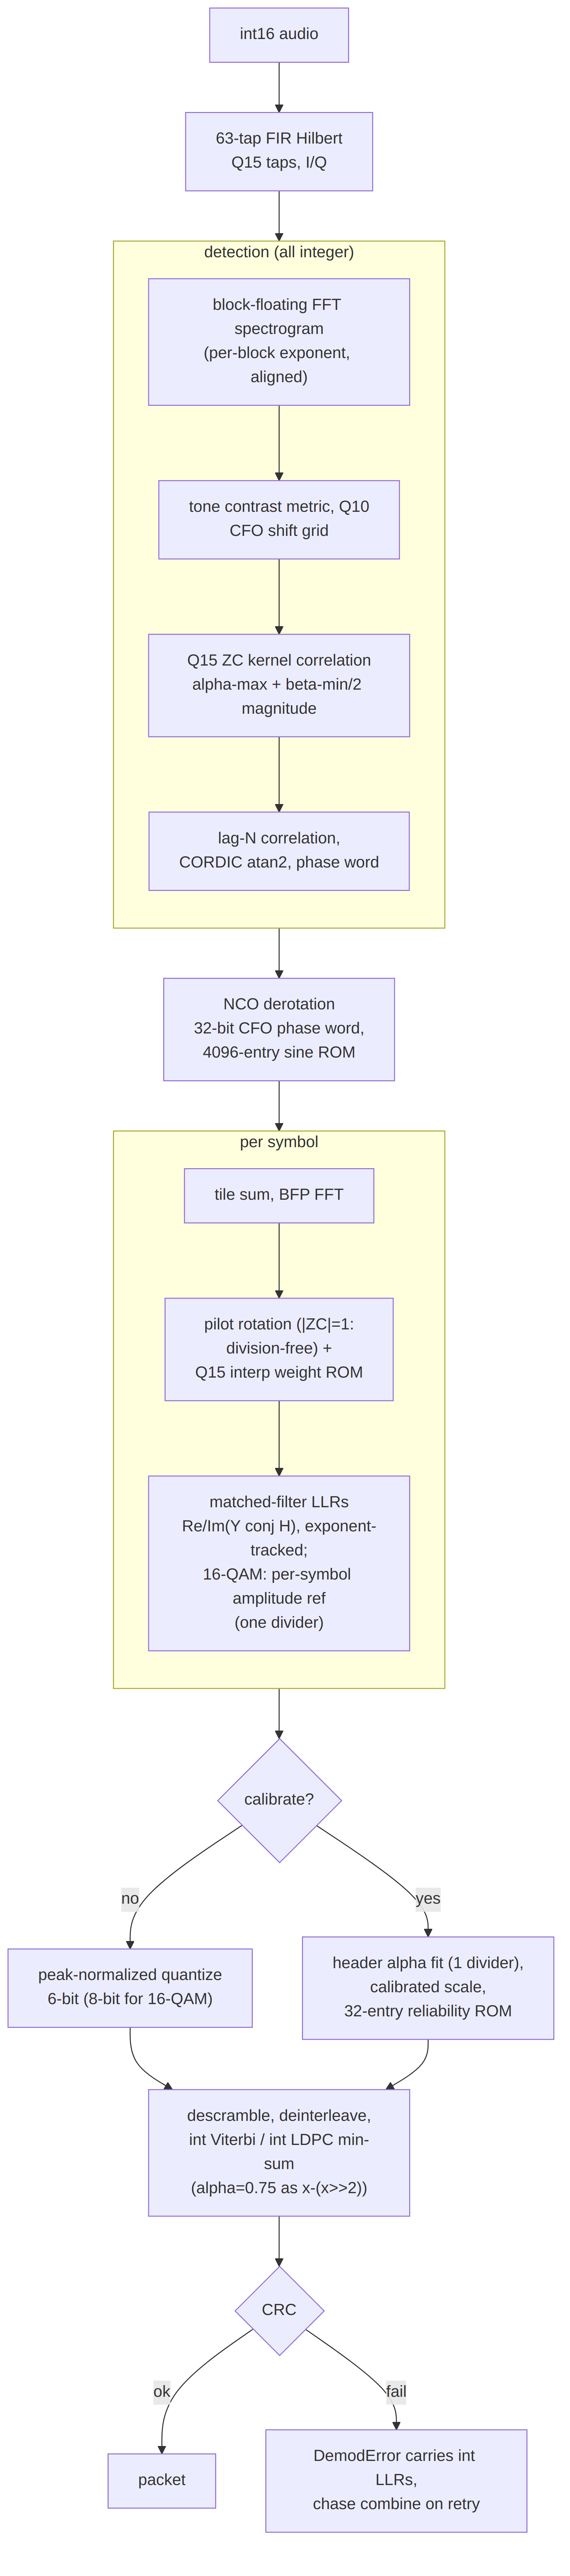
\includegraphics[width=0.8\textwidth,height=0.62\textheight,keepaspectratio]{images/fixed_rx.png}
    \caption{Fixed-point receiver datapath (all integer).}
    \label{fig:fixed_rx}
\end{figure}

\subsection{Primitive Blocks}

\begin{table}[H]
    \centering
    \caption{Fixed-point primitives and their measured quality.}
    \label{tab:fixed_prims}
    \small
    \begin{tabular}{@{}lp{7.2cm}l@{}}
    \toprule
    \textbf{Block} & \textbf{Structure} & \textbf{Quality} \\
    \midrule
    FFT     & radix-2 DIT, Q15 twiddle ROM, per-stage $\gg 1$
              (built-in $1/N$), BFP wrapper & 59\,dB SQNR \\
    Hilbert & 63-tap type-III FIR, Q15 & 61\,dB SQNR \\
    NCO     & 32-bit phase accumulator, 4096-entry Q15 sine ROM &
              $-67$\,dBc \\
    CORDIC  & 16-iteration vectoring, angle in phase-word units &
              $<0.001$\,rad \\
    Viterbi & 6-bit LLRs (8-bit for 16-QAM data), $\pm 1$ expected
              symbols (adds only), int32 metrics & exact \\
    LDPC    & integer normalized min-sum,
              $\alpha = x - (x \!\gg\! 2)$ & matches float min-sum \\
    \bottomrule
    \end{tabular}
\end{table}

\subsection{RTL-Oriented Conventions}

\begin{itemize}
    \item \textbf{CFO is a 32-bit phase-increment word} end-to-end (one
          turn $= 2^{32}$); Hz exists only at API boundaries.
    \item \textbf{Divisions are minimised.}  Channel estimation is
          division-free ($|$ZC pilot$| = 1$, so the estimate is a
          rotation); pilot interpolation is a Q15 weight ROM.  The
          remaining dividers: the calibration $\alpha$ fit (one per
          frame), the 16-QAM amplitude reference (one per symbol), and
          the detection metrics.
    \item \textbf{Scale tracking.}  BFP exponents are carried through
          every energy and LLR comparison (scale
          $\propto 2^{2\cdot\mathrm{exp}}$); ZC correlation magnitude
          uses the $\alpha$-max~+~$\beta$-min/2 approximation.
\end{itemize}

Two intentional deltas versus the float model: NORMAL-mode tone
detection uses a 256-point FFT (float: 128) so the coarse CFO grid is
fine enough for an unambiguous lag-$N$ residual; and the demodulator
uses the slew-limited frequency-search tracker for \emph{all} tile
factors --- the float model's polynomial phase fit is not RTL-friendly,
and measurably weaker at the edge anyway.

\subsection{Measured Results and One Surprise}

The fixed TX waveform correlates 0.99998 with the float waveform; the
full fixed/float TX$\times$RX cross-matrix decodes; NORMAL-mode PER is
within $\approx$0.5\,dB of the float receiver, and ROBUST/EXTREME
decode at $-11/-17$\,dB.  The surprise: the default 6-bit
peak-normalized LLR quantization already acts as a \emph{compressive
recalibration} (Section~\ref{sec:llr}), and combined with the
frequency-search tracker the fixed receiver \textbf{matches or beats
the recalibrated float chain at $-9/-10$\,dB} (22 vs.\ 20 and 11 vs.\ 5
of 30 trials).  The calibrated-LLR mode (integer header $\alpha$ fit
plus a 32-entry reliability ROM measured on the fixed chain itself)
therefore buys a \emph{stable cross-frame LLR scale} --- what makes
HARQ combining legitimate --- rather than extra PER.

The 16-QAM rungs were swept separately
(\texttt{experiments/fixed\_qam16\_sweep.py}, 48 packets/point, fixed
TX with identical samples into both receivers).  The first sweep
exposed a $\sim$2\,dB gap on the puncture-weak high rates
($+4.6/+6.3$\,dB versus float $+2.6/+4.5$ at rates 2/3 and 3/4):
16-QAM max-log LLRs span a much wider dynamic range than BPSK
(inner/outer bits times per-carrier gain), and the 6-bit
peak-normalized quantization compresses them.  The fix is a
\emph{per-modulation quantizer}: data blocks with $\mu = 4$ use an
8-bit peak-normalized quantizer ($\pm 127$), while $\mu \le 2$ keeps
the 6-bit path, whose compression is precisely what helps at the BPSK
edge.  Peak and mean normalization measured equivalent at 8 bits ---
the win is the resolution --- so the RTL cost is two extra LLR bits on
the 16-QAM data path only.  Re-swept, the fixed receiver measures
$+1.5/+2.9/+5.3$\,dB for rates 1/2, 2/3, 3/4: within 0.3--0.8\,dB of
the float receiver everywhere.

Robustness note: the tiled chain survives up to 65\,\% contiguous
audio erasure (the $4\times$ tiles keep partial symbols alive); the
HARQ path is validated by a deterministic test with two 75\,\%
complementary erasures whose union covers every sample at least once.

\subsection{Gated Two-Stage Frequency Search}

The first-symbol residual-CFO search --- 275 full-symbol hypotheses at
EXTREME, the demodulator's dominant burst in a firmware budget --- was
restructured as coarse-then-fine: a quarter-length coarse pass
(tiles/4 accumulation, whose $4\times$ wider frequency mainlobe
tolerates a $4\times$ coarser grid) ranks hypotheses, and only the
top-3 $\pm 5$-step windows run at full precision, $\approx$5.5$\times$
fewer derotated samples.  The coarse metric is $\sim$6\,dB noisier
than the full symbol, and a hard coarse decision measurably costs
$\sim$0.5\,dB at the EXTREME sensitivity edge --- so the fast path is
taken only when the coarse top-1/median contrast clears a measured
gate ($2.25\times$; edge frames sit $\le 2.2\times$, frames with
5\,dB of margin $\ge 2.7\times$), and below it the exhaustive grid
runs unchanged.  The same gated structure was then back-ported to the
\emph{float} demodulator's per-symbol frequency search --- where it
pays on every symbol, not just the first, because the float chain has
no slew-limited tracker.  Figure~\ref{fig:coarse_ab} shows the
noise-sensitivity A/B (\texttt{experiments/coarse\_search\_ab.py},
36 packets/point, identical channel realizations per arm), including
the ablation that justifies the gate: the quarter-length coarse pass
\emph{without} the gate (dotted) shifts the EXTREME waterfall right by
0.5--1\,dB (fixed RX at $-18$\,dB: PER 0.31 vs.\ 0.11), while the
gated search (dashed) is \emph{identical} to the exhaustive grid at
every measured point, both models --- lossless by construction, with
the full grid reduced to a low-margin fallback.  ROBUST tolerates
even the ungated coarse pass at parity: its coarse stage (4 of 16
tiles) retains enough detector SNR at that mode's shallower edge, so
the gate specifically protects the deepest mode.

\begin{figure}[H]
    \centering
    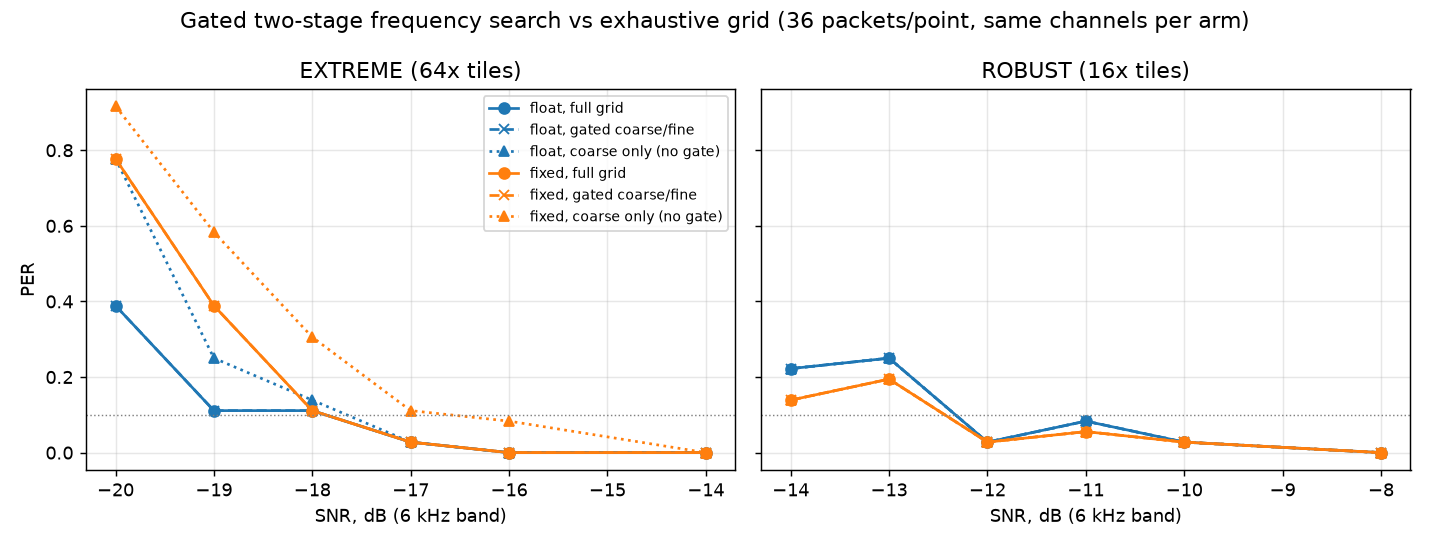
\includegraphics[width=\textwidth]{images/coarse_search_ab.png}
    \caption{PER versus SNR for the exhaustive frequency grid (solid),
             the gated two-stage search (dashed), and the ungated
             coarse-only ablation (dotted); float and fixed-point
             receivers, same channels per arm.  Gated overlays full
             exactly everywhere; the ablation's edge loss in the
             EXTREME panel is what the contrast gate prevents.}
    \label{fig:coarse_ab}
\end{figure}

\subsection{Integer SNR Estimator and Full-System Integration}

Rate adaptation is driven by a per-frame SNR estimate the fixed
receiver originally lacked.  The added estimator is data-aided and
divider-free: per-column first/second moments of the LLR stream
against the known $\pm 1$ bits (the re-encoded header always, plus the
decoded data block for $\mu \le 2$), an integer $\log_2$ via bit-length
and a 16-entry mantissa ROM, minus the tiling gain, plus one measured
global calibration constant ($-7.2$\,dB, constant across all modes and
modulations).  Two design points were forced by measurement.  First,
grouping moments \emph{per column} removes the multipath $|H|^2$
spread across carriers.  Second, symbol rows must be
\emph{gain-weighted} by their mean $|$LLR$|$: a tiled EXTREME frame
spans several QSB fade cycles, and both naive poolings failed ---
unweighted moments count the fading itself as noise (measured
5--15\,dB pessimistic, which parked the rate ladder at rung~0), and
equal-weight gain-normalized pooling yields a harmonic-mean-flavored
estimate still dominated by fade valleys.  Gain weighting reproduces
the signal-energy-weighted average the float estimator reports --- the
statistic the ladder was tuned against --- and reduces to the plain
estimator when the gain is constant.  Final accuracy:
$\le$1.5\,dB error over $-17\ldots+8$\,dB, every mode and modulation
(slightly pessimistic on the tiled modes, the safe direction).

With the estimator in place, a thin adapter (\texttt{FixedPHY}) gives
the fixed TX/RX the float \texttt{Transceiver}'s link-facing interface
--- including blind mode auto-detection by trying the three per-mode
receivers --- and \texttt{LinkStation} accepts it via a \texttt{phy}
parameter.  The complete adaptive system then runs on the integer
pipeline end to end: \texttt{demo\_wav.py -{}-phy fixed} records the
two-station QSO of Section~\ref{sec:results} with both stations
\emph{and} the blind monitor decoding on fixed point.  At
$-2/-1$\,dB the session bootstraps at EXTREME, netting and climbing
exactly as the float system does, and the monitor blind-decodes 37 of
47 frames; at $+5$\,dB the ladder climbs into 16-QAM (rungs 9--10 on
the air, requests up to rung~11) and the monitor decodes 26 of 40
(Appendix~\ref{app:fixeddemo}).

\subsection{Debug Lore}

Three integer-domain bugs cost real time and are recorded so an RTL
implementation does not repeat them: the ZC metric's Q-scaling must
account for \emph{both} $2^{-15}$ factors the Q15 kernel introduces (a
perfect correlation scored 0.006 with one missing); scipy's
\texttt{remez(..., type="hilbert")} returns taps producing $-\sin$ for
a cosine input, so the taps must be negated for a positive-frequency
analytic signal; and BFP energies compare only after shifting by
$2\,\Delta\mathrm{exp}$.

\section{Validation and Results}
\label{sec:results}

\subsection{Regression Suites}

Every layer has a self-verifying suite
(Table~\ref{tab:suites}); all pass at the state documented here.

\begin{table}[H]
    \centering
    \caption{Verification suite summary.}
    \label{tab:suites}
    \small
    \begin{tabular}{@{}lrp{7.6cm}@{}}
    \toprule
    \textbf{Suite} & \textbf{Checks} & \textbf{Scope} \\
    \midrule
    \texttt{verify\_article.py} & 44 & bit-exact article worked examples:
        CRCs, Base38/QTH, conv-code outputs at all rates,
        scrambler/interleaver sequences, ZC ACF
        (Appendix~\ref{app:verify}) \\
    \texttt{smoke\_e2e.py}      & 10 & end-to-end TX$\to$channel$\to$RX
        incl.\ CFO, modes, STF, auto-mode detection \\
    \texttt{fixed\_point.py}    & 24 & fixed-point primitives, TX/RX
        parity, LDPC and 16-QAM TX and RX, HARQ, calibration, SNR
        estimator (Appendix~\ref{app:fixed}) \\
    \texttt{rf\_channel.py}     &  6 & SSB transparency, LO-derived CFO
        to 0.1\,Hz, decode through the fading RF chain \\
    \texttt{afc\_netting.py}    & --- & netting convergence +
        trim-budget and anchor guard scenarios (PASS/FAIL) \\
    \texttt{simplex\_session.py}& --- & whole-system two-station test,
        bit-exact delivery assert (PASS/FAIL) \\
    \bottomrule
    \end{tabular}
\end{table}

\subsection{Article Reproduction}

\begin{table}[H]
    \centering
    \caption{Reproduction versus the article.}
    \label{tab:reproduction}
    \small
    \begin{tabular}{@{}lll@{}}
    \toprule
    \textbf{Metric} & \textbf{Article} & \textbf{This implementation} \\
    \midrule
    Worked examples & --- & 44/44 bit-exact \\
    Sensitivity, BPSK 1/3 & $\approx -7.5$\,dB &
        $-7.2$\,dB raw RX; $-7.6$\,dB genie-synchronized \\
    BER/PER curves (Figs.~23--24) & simulated &
        reproduced (Figure~\ref{fig:berper}), both preambles \\
    \bottomrule
    \end{tabular}
\end{table}

The remaining 0.3\,dB between the raw and genie-synchronized receiver
is residual synchronization loss at low SNR (occasional missed
detections and one-symbol timing slips), not the decode chain ---
i.e.\ the reproduction gap is closed to within measurement noise of
its diagnosed cause.

\begin{figure}[H]
    \centering
    \begin{subfigure}{0.49\textwidth}
        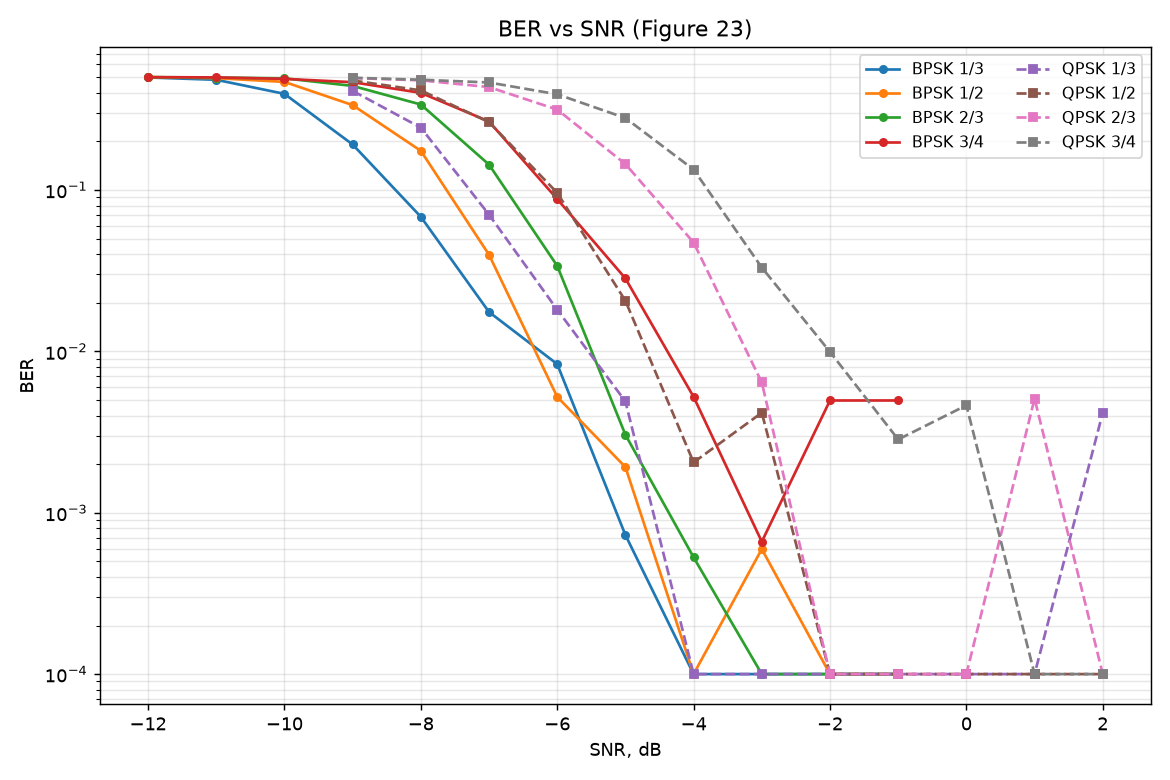
\includegraphics[width=\textwidth]{images/ber_vs_snr.png}
        \caption{BER versus SNR.}
    \end{subfigure}
    \hfill
    \begin{subfigure}{0.49\textwidth}
        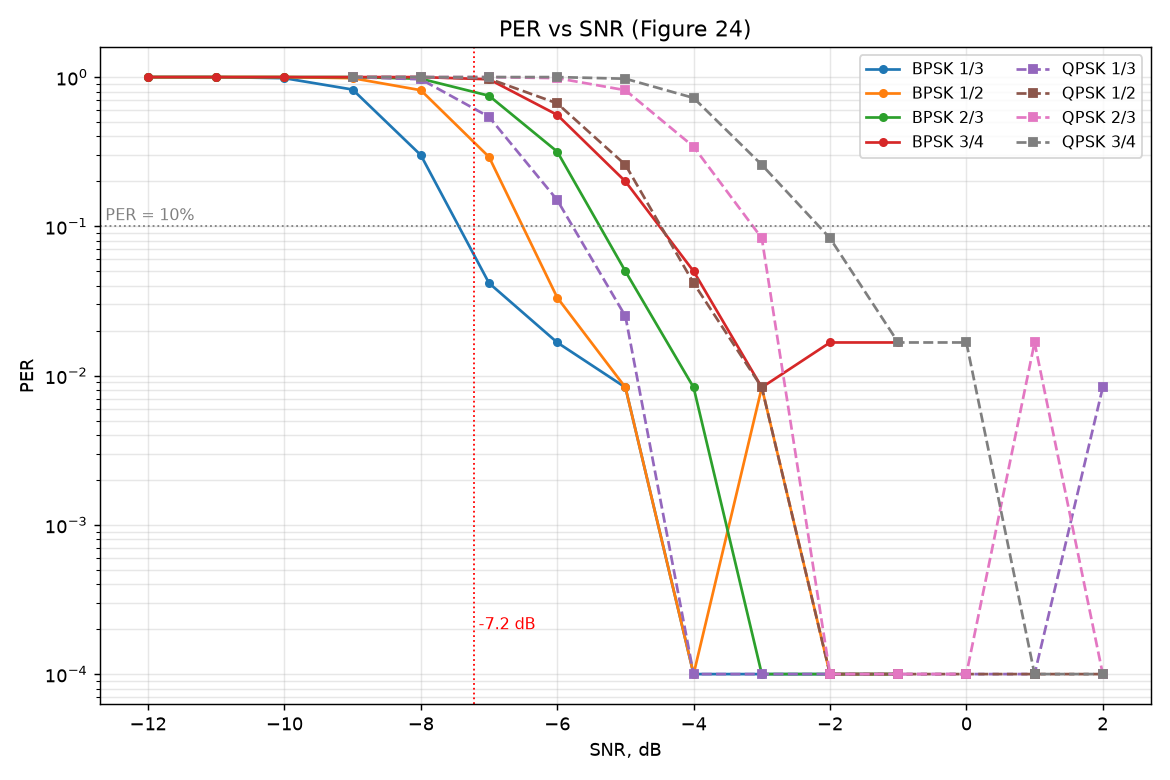
\includegraphics[width=\textwidth]{images/per_vs_snr.png}
        \caption{PER versus SNR.}
    \end{subfigure}
    \caption{Reproduction of the article's Figures~23--24: eight
             modulation/rate configurations over the article channel
             model (multipath $[1,0,0.4,0,0,0.2]$, BSC $10^{-3}$, BEC
             $2\cdot 10^{-2}$, random $\pm 100$\,Hz CFO with drift,
             random timing), 120 packets per point.}
    \label{fig:berper}
\end{figure}

\begin{figure}[H]
    \centering
    \begin{subfigure}{0.49\textwidth}
        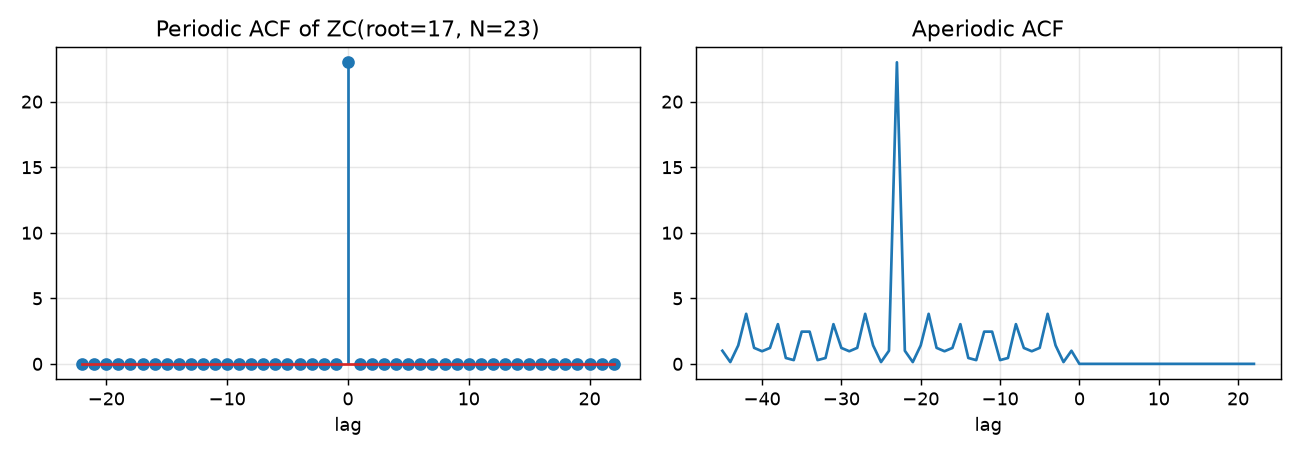
\includegraphics[width=\textwidth]{images/zc_acf.png}
        \caption{Zadoff--Chu autocorrelation.}
    \end{subfigure}
    \hfill
    \begin{subfigure}{0.49\textwidth}
        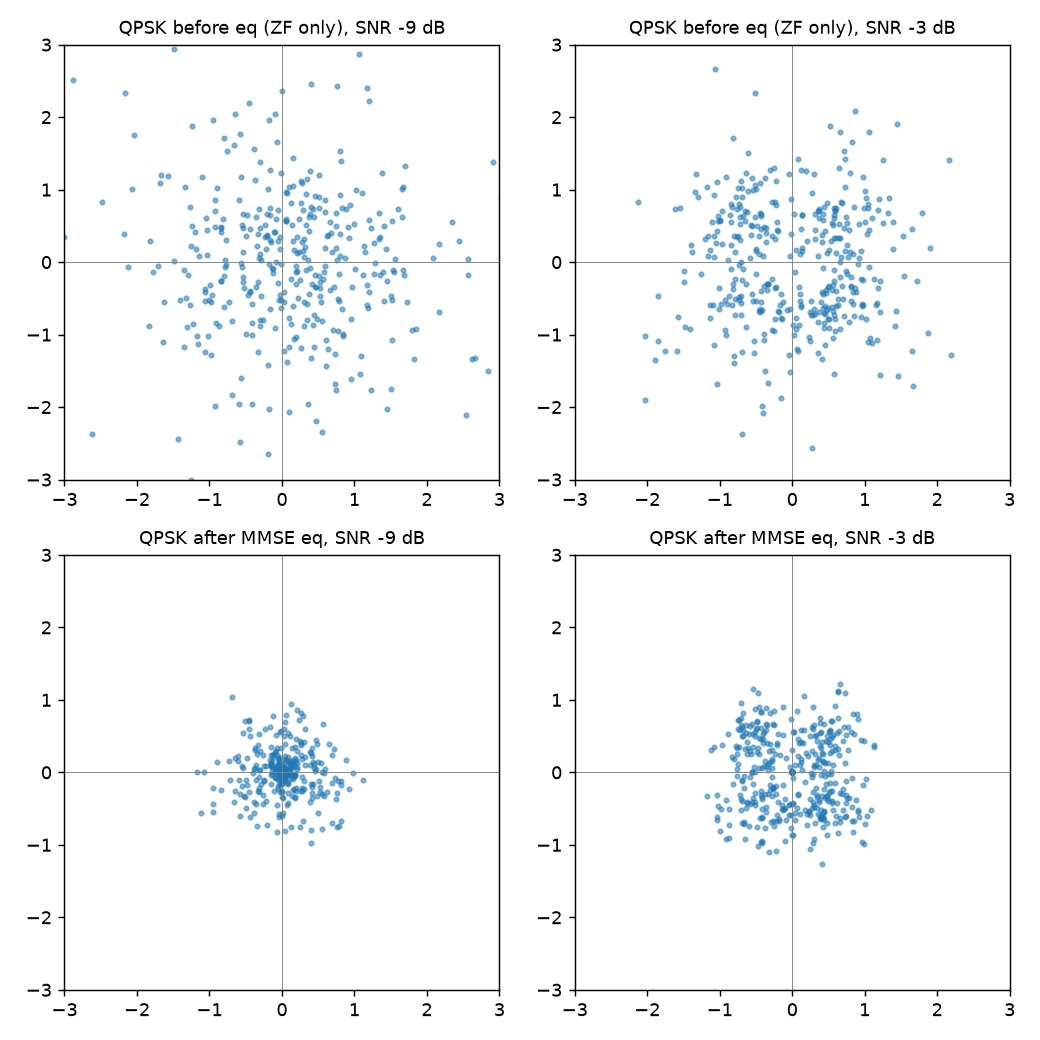
\includegraphics[width=\textwidth]{images/constellation_qpsk.png}
        \caption{QPSK constellation, before/after equalization.}
    \end{subfigure}
    \caption{Article-style diagnostic figures
             (\texttt{experiments/figures.py}).}
    \label{fig:diag}
\end{figure}

\subsection{Measured Feature Gains}

Table~\ref{tab:gains} consolidates every A/B-measured improvement.
All A/B comparisons use fixed seeds (same channel realizations per
arm); sensitivity points use 40--120 trials.

\begin{table}[H]
    \centering
    \caption{Feature gains, A/B measured.}
    \label{tab:gains}
    \small
    \begin{tabular}{@{}p{4.6cm}p{9.6cm}@{}}
    \toprule
    \textbf{Feature} & \textbf{Measured effect} \\
    \midrule
    LLR recalibration & $+1.5$--2\,dB on BPSK/QPSK rungs ($-9$\,dB:
        6/40 $\to$ 29/40); regresses 16-QAM $\to$ gated to
        $\mu \le 2$ \\
    HARQ chase combining & 2nd attempt 15/20 vs.\ 10/20 at
        $-8.5$\,dB (noise-limited regime) \\
    LDPC (IRA 768/256) vs.\ conv & $+0.7$\,dB AWGN at BLER 10\,\%;
        $\approx$ parity end-to-end (front-end LLR quality binds) \\
    STF preamble variant & equal to Newman everywhere ($\pm 0.14$\,dB
        over 8 configs, $2\sigma$ agreement per point) \\
    AFC netting & $+284$\,Hz $\to$ $<12$\,Hz in 5 exchanges; steady
        $\le 11$\,Hz under 0.09\,Hz/s relative drift \\
    Fixed-point RX vs.\ float & $\le 0.5$\,dB loss at $-7$\,dB;
        \emph{ahead} at $-9/-10$\,dB (22 vs.\ 20, 11 vs.\ 5 of 30,
        against float+recal); 16-QAM within 0.3--0.8\,dB after
        per-modulation LLR quantization (8-bit for $\mu = 4$) \\
    Integer SNR estimator & $\le$1.5\,dB error, $-17\ldots+8$\,dB, all
        modes; gain weighting essential (equal-weight pooling was
        5--15\,dB pessimistic on faded EXTREME frames) \\
    \bottomrule
    \end{tabular}
\end{table}

\subsection{The System Demonstration}

The recorded demonstration (\texttt{results/system\_demo.wav},
Figure~\ref{fig:timeline}, transcript in Appendix~\ref{app:demo}) is
the whole system at once: two stations over the fading SSB RF chain
with realistic LO errors, EXTREME-mode negotiation, rate climb,
AFC netting visible in the transcript's CFO column, HARQ, and
bidirectional message transfer --- blind-decoded from the monitor's
audio by \texttt{demod\_frame\_auto} with no side information.

\begin{figure}[H]
    \centering
    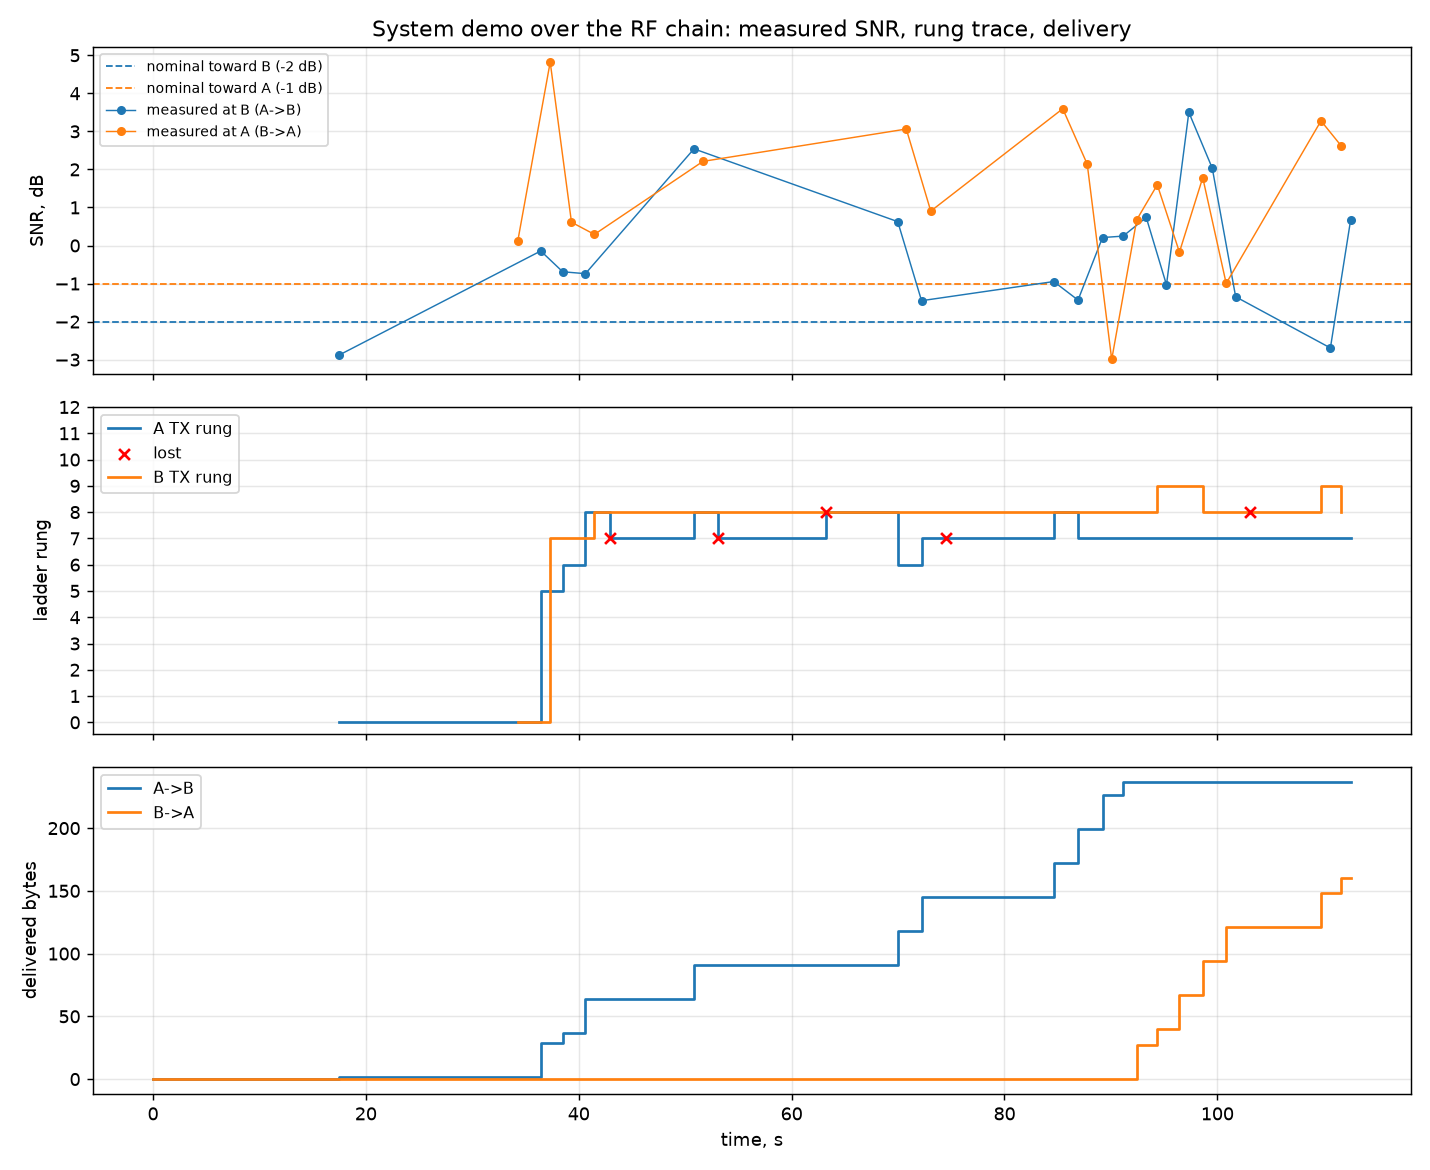
\includegraphics[width=\textwidth]{images/system_demo_timeline.png}
    \caption{System-demo timeline: per-frame SNR, ladder rungs, and
             delivery over the session.}
    \label{fig:timeline}
\end{figure}

The same demonstration also exists on the \emph{fixed-point} pipeline
(\texttt{-{}-phy fixed}, Section~\ref{sec:fixed}): at $-2/-1$\,dB
(\texttt{system\_demo\_fixed.wav}, 37/47 frames blind-decoded) and at
$+5$\,dB, where the ladder climbs into 16-QAM
(\texttt{system\_demo\_fixed\_qam16.wav}, 26/40;
Figure~\ref{fig:fixed_timeline} and Appendix~\ref{app:fixeddemo}).

\begin{figure}[H]
    \centering
    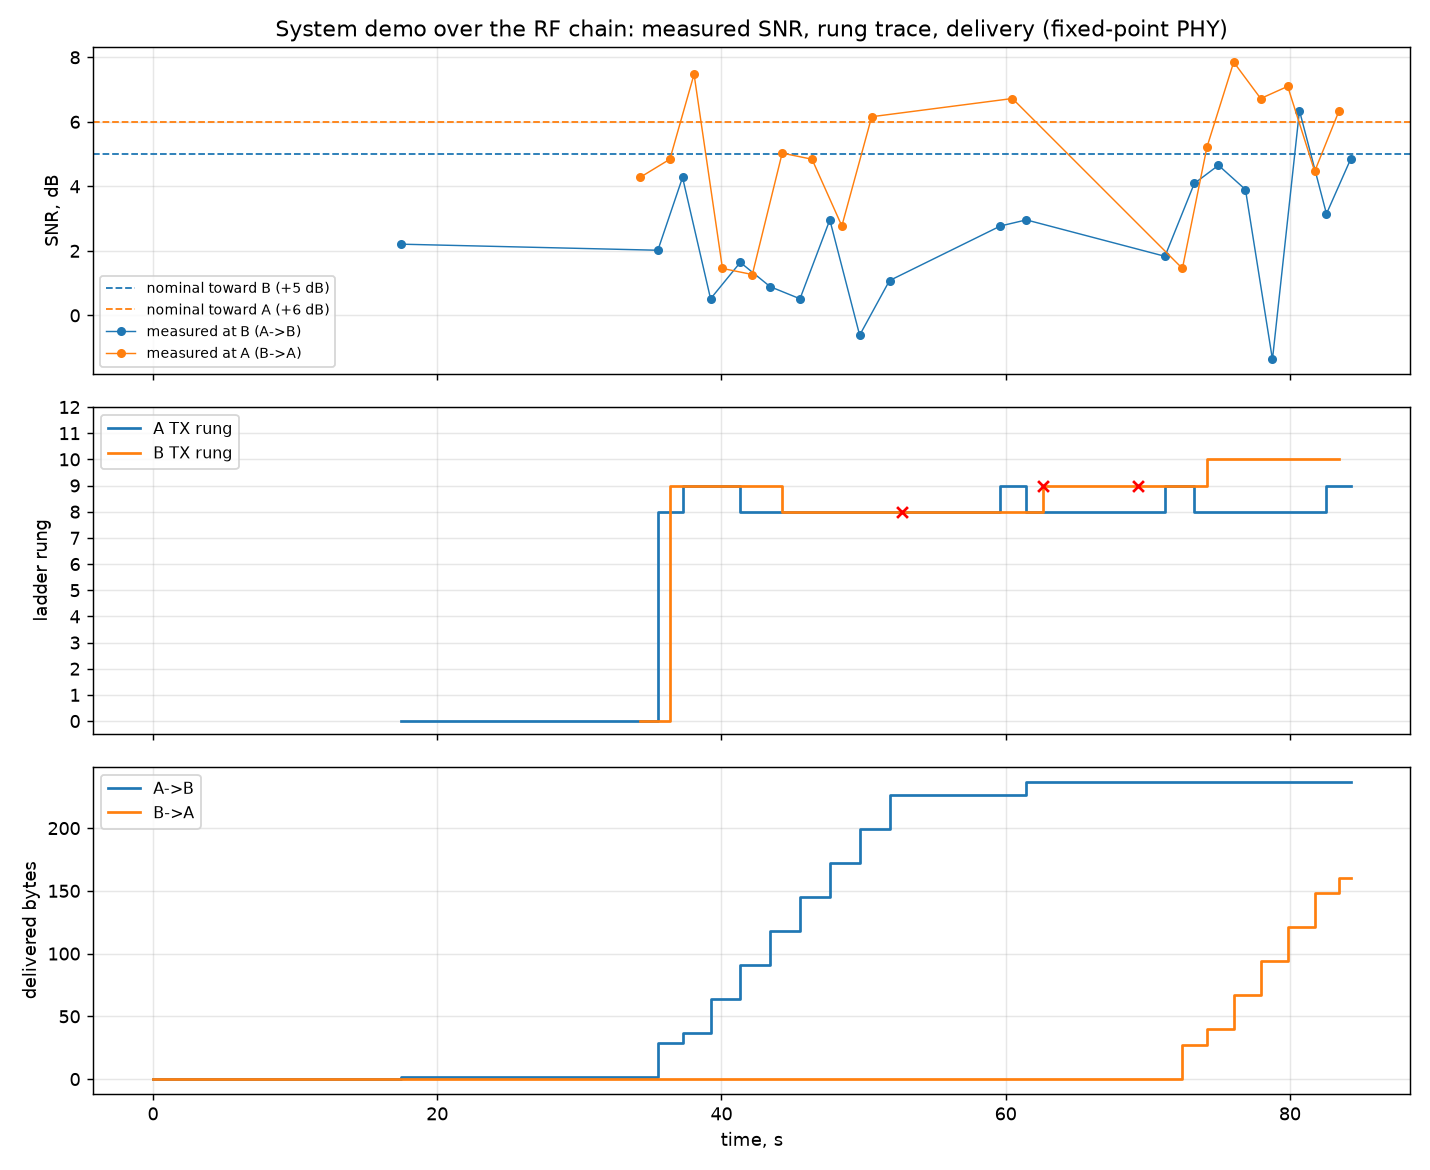
\includegraphics[width=\textwidth]{images/system_demo_fixed_qam16_timeline.png}
    \caption{Fixed-point-pipeline demo at $+5$\,dB: the integer SNR
             estimates drive the ladder into the 16-QAM rungs.}
    \label{fig:fixed_timeline}
\end{figure}

\subsection{Link Budget}

In radio terms, the EXTREME operating point ($-17.5$\,dB planned,
$-17.9$\,dB measured, 6\,kHz reference) needs
$S/N_0 \approx +20.3$\,dB-Hz, i.e.\ $\approx -13.7$\,dB in the
ham-standard 2.5\,kHz bandwidth --- about 7\,dB less sensitive than
FT8~\cite{ft8} and $\sim$20\,dB better than SSB voice.  Against
ITU-R~P.372 noise levels~\cite{itu_p372} with 0\,dBi antennas: on
80\,m at 10\,W, 500--2000\,km reliably on typical nights and
3000--5000\,km from quiet rural sites; on 40\,m at 10\,W,
300--1500\,km all day and worldwide multi-hop on quiet winter nights;
100\,W adds roughly one ionospheric hop to everything.  A planning
caveat: EXTREME's 0.69\,s coherent integration assumes
$\lesssim$0.1\,Hz Doppler spread --- on disturbed or auroral paths
($\ge$1\,Hz) the coherent gain collapses at any power and ROBUST is
the better choice, one more argument for adaptive mode selection.

\subsubsection{Measured Against a Reference Source}
\label{sec:link_budget_measured}

Everything above is derived from a \emph{relative} sensitivity and an
\emph{assumed} noise figure.  With the SDR receiver of
Section~\ref{sec:cport_sdr} on the bench, the assumption can be
replaced by a measurement: a tinySA's calibration output, a reference
tone at a documented level, was fed into the radio through a 40\,dB
attenuator and the receive chain characterised end to end
(\texttt{demoapp/sdr\_rx\_calibrate.py};
\texttt{results/sdr\_rx\_calibration.csv}).  At 10\,MHz with
$-65$\,dBm at the antenna port:

\begin{table}[H]
    \centering
    \caption{Receive chain measured against a reference source
             (HackRF One, LNA 40\,dB).}
    \label{tab:rx_calibration}
    \small
    \begin{tabular}{@{}lp{8.2cm}@{}}
    \toprule
    \textbf{Quantity} & \textbf{Measured} \\
    \midrule
    Frequency error & $-33.1$\,Hz at 10\,MHz $= -3.31$\,ppm, repeatable
                      to 0.0\,Hz ($-23$\,Hz at 7\,MHz) \\
    Linearity       & 1.002\,dB/dB over 16\,dB of gain, 0.03\,dB
                      residual \\
    Receiver noise  & $-95.5$\,dBm in the 6\,kHz reference band
                      (NF $\approx$ 40\,dB) \\
    \midrule
    \multicolumn{2}{@{}l}{\textit{Absolute sensitivity} $=$ measured
      noise floor $+$ the rung's required SNR:} \\
    rung 0 \; EXTREME BPSK 1/3 \; 7.8\,bit/s   & $-113.4$\,dBm \\
    rung 4 \; NORMAL BPSK 1/3 \; 117.6\,bit/s  & $-103.1$\,dBm \\
    rung 12 \; NORMAL 16-QAM 3/4 \; 1059\,bit/s & $-90.8$\,dBm \\
    \bottomrule
    \end{tabular}
\end{table}

Two results matter for planning.  First, the receiver's own noise is
\emph{not} what limits this link: against ITU-R~P.372 atmospheric noise
in the same 6\,kHz band, external noise still dominates by $+9$\,dB at
a quiet rural site, $+17$\,dB at a typical rural one and $+24$\,dB in
residential noise --- so the externally-limited assumption behind the
ranges above holds, and it holds with about 9\,dB of margin at the
quietest sites.  That margin is precisely where a preselector and a
low-noise amplifier begin to pay for themselves, and it is worth noting
that the 40\,dB noise figure measured here belongs to a wideband,
8-bit, unpreselected SDR --- an ordinary HF receiver is far better, so
this is close to a worst case.

Second, the frequency error is negligible for this waveform: 3.31\,ppm
against an acquisition range that tolerates roughly 50\,ppm at 7\,MHz.
A free-running SDR needs no external reference to \emph{acquire} a
frame; a disciplined oscillator matters only for EXTREME's 0.69\,s
coherent integration, where drift \emph{within} a 44\,s frame is the
constraint rather than absolute accuracy.  The absolute levels in
Table~\ref{tab:rx_calibration} inherit the calibration output's nominal
$-25$\,dBm; the relative results --- linearity, frequency error, and
the comparison against atmospheric noise --- do not.

\section{C Implementation and Infrastructure}
\label{sec:cport}

The fixed-point reference model of Section~\ref{sec:fixed} answers
\emph{whether} integer arithmetic preserves the link performance; the C
port (\texttt{cport/}) answers whether the system \emph{fits} a DSP or
microcontroller.  It is portable C99 with no \texttt{malloc} and no
floating point on the signal path (doubles remain on the control plane
--- dB values and timers --- as in the model), and covers the entire
feature family: both FEC families, all three modulations and link
modes, the gated two-stage frequency search, HARQ combining, calibrated
LLRs, the integer SNR estimator, the full link layer, and a streaming
receiver architecture for MCU deployment.

\subsection{Bit-Exact Porting Methodology}
\label{sec:cport_method}

Every module is validated against \emph{golden vectors} generated from
the Python fixed-point model (\texttt{gen\_vectors.py}): inputs and
expected outputs are dumped as C headers and compared with
\texttt{memcmp} --- no tolerances anywhere.  Whole transmit frames
(up to 260\,k samples for EXTREME) are compared through 64-bit
FNV-1a hashes over every \texttt{int16} sample, with the first 64
samples embedded verbatim for debuggability.  Two rules keep the
comparison honest:

\begin{itemize}
    \item \textbf{ROMs are dumped, never recomputed.}  Twiddles,
          preamble blocks, pilot symbols, LDPC graph, ladder tables and
          detection kernels all come from the Python model; a C-side
          reimplementation of table generation would risk silently
          diverging in rounding.
    \item \textbf{Width findings are documented, not patched over.}
          Every intermediate that exceeds a naive width estimate
          (Viterbi path metrics, BFP energy sums, the ZC metric's
          Q-scaling) is recorded in \texttt{WIDTHS.md} with its measured
          range, so an RTL implementation inherits the analysis.
\end{itemize}

The suite currently runs \textbf{79 checks} across six binaries
(primitives, bit pipeline, TX frames, RX demodulation, streaming
receiver, link layer).  RX genie vectors are self-hosting: clean frames
are rebuilt by the bit-exact C transmitter inside the test, so only the
Python detection genie (start sample, CFO word) and expected bits are
dumped.

\subsection{Streaming Receiver}
\label{sec:cport_stream}

The frame-at-once reference receiver is impractical on an MCU (it wants
the whole capture in memory), so \texttt{rx\_stream.c} implements a
ring-buffer state machine (\textsc{search} $\rightarrow$ \textsc{zc}
$\rightarrow$ \textsc{header} $\rightarrow$ \textsc{data}) fed in
arbitrary chunks.  The tone-detection stage is necessarily causal and
diverges from the model in two documented ways: block exponents and the
noise floor are windowed (a streaming receiver cannot know the whole
capture's minimum exponent, and the model's whole-capture \emph{median}
floor is acausal), and detection commits on a local metric peak ---
when the above-threshold region ends or the argmax stays stable for a
full window span --- instead of a global argmax.  On the golden corpus
the streaming receiver lands on the identical tone anchor for clean
frames, making everything downstream bit-identical to the
frame-at-once path.

Memory is dominated by sample history, and two measurements shaped the
final architecture:

\begin{itemize}
    \item \textbf{The ring only needs to cover the Zadoff--Chu
          re-anchor lookback, not the preamble.}  The tone stage is
          incremental (each 512-sample block folds into a
          $\approx$540-byte summary; raw tone samples are never
          re-read).  A permanent high-water-mark diagnostic
          (\texttt{rxs\_ring\_hwm}) measured the deepest lookback over
          the corpus at 8\,510 / 32\,318 / 124\,478 samples per mode.
    \item \textbf{One shared raw ring serves every instance.}  All
          mode-instances listen to the same audio (the preamble root
          self-labels the mode), so concurrent instances write
          identical samples and a single \texttt{int16} ring of
          147\,456 samples (288\,KB) replaces per-instance analytic
          rings.  The analytic signal is reconstructed on extraction
          (Hilbert-on-read), bit-identical to the former write-time
          FIR --- and measured \emph{faster}, because the 63-tap filter
          now runs only on consumed regions rather than on every
          sample in every instance.
\end{itemize}

\subsection{Protocol Extensions}
\label{sec:cport_proto}

Three extensions beyond the Python reference address the fixed
per-frame overhead (preamble + header $\approx$0.64\,s in NORMAL mode)
that dominates air time at the top rungs:

\begin{itemize}
    \item \textbf{Selective-repeat burst ARQ.}  Bulk transfers send up
          to a window of frames back-to-back, answered by one bitmap
          acknowledgment (NACK-by-omission).  The two flag combinations
          impossible in the legacy protocol serve as burst frame types,
          so the legacy path is untouched.
    \item \textbf{Extended frames.}  The article's header \texttt{len}
          field counts packet \emph{bits} (255 max
          $\rightarrow$ 27-byte payloads).  An unused header type
          codepoint reinterprets \texttt{len} as payload \emph{bytes},
          allowing 255-byte payloads (2\,076-bit packets) behind a
          single preamble.  Burst fragment size scales with the
          engage-time rung (200\,B at rung $\ge$10, 100\,B at $\ge$7,
          else 25\,B).
    \item \textbf{Streamed burst windows.}  A whole selective-repeat
          window is transmitted behind one preamble and header
          (Sections~\ref{sec:stream} and~\ref{sec:burstwin}) instead
          of one preamble per fragment.  \texttt{tx\_build\_burst}
          waveforms are bit-exact against the fixed-point model, and
          both receivers can follow a burst: the frame-at-once path
          re-runs the recording through \texttt{rxd\_receive\_burst}
          and re-locks on each Zadoff--Chu block, while the streaming
          receiver steps to the next block at its deterministic offset
          via \texttt{rxs\_continue\_burst}.
\end{itemize}

A streamed burst carries only full-size fragments; the short tail of a
transfer always travels as its own frame, because the receiver derives
the message length from that final fragment's own length.  The
acknowledgment request rides on the burst's \emph{first} block as well
as its last, so a peer that cannot follow the stream still answers and
the sender learns by bitmap rather than by waiting out a timeout.

That receive-side continuation is also where the sharpest bug of this
work appeared.  While the streaming receiver is stepping through
blocks it is not running the preamble detector, so a continuation that
does not know where to stop makes the receiver deaf for one block-time
per phantom block.  An early version re-armed its block counter on
every successful block and therefore never learned that a burst had
ended: it chased up to seven blocks that were never sent,
$\approx$12\,s of deafness landing squarely on the peer's next burst,
which timed out and retried indefinitely.  The transmitter marks the
last block of a burst with the acknowledgment request, which is the
stop signal --- qualified as ``set \emph{and} not the first block of
this stream'', since the first carries it too.

Measured on the virtual channel: a 250-byte transfer completes in
3 frames instead of $\approx$20 for stop-and-wait, and a 5\,000-byte
file drops from 211 transmitted frames (legacy) to 45, holding the top
QAM16 rung throughout.  Streaming the window compounds this: a
250-byte transfer at 25-byte fragments takes 4 transmissions streamed
against 13 after falling back to per-frame bursts, and a 14\,kB file
over a $+20$\,dB channel takes 76 transmissions streamed against 187
per-frame.

A fourth extension sits above the protocol rather than inside it.
Nothing in the chain compressed, while every comparable HF system does
--- Winlink's B2F, VARA, and PACTOR all compress before transmitting.
Files are now DEFLATEd whole and the compressed stream is what gets
split into parts; compressing each part separately would discard most
of the ratio, since the dictionary never warms up.  A distinct envelope
magic marks the compressed form, so a peer that predates it sees an
unknown message rather than misparsing a structurally valid one, and
the transmitter falls back to sending raw whenever compression fails to
shrink the payload.  Compression lives at the application layer
precisely so the C port stays dependency-free: an embedded build
substitutes miniz or heatshrink, with plain DEFLATE on the wire either
way.  Measured on a 14\,kB configuration file: 14\,162 bytes to
5\,015 on air, $2.82\times$.  The honest qualification is that
transmissions fell only $1.4\times$ and wall-clock delivery
$1.6\times$, because acknowledgments and the rate-ladder bootstrap do
not compress --- the ratio applies to the part of an exchange that is
payload, not to the exchange.  Supporting endpoints added alongside: a
diagnostic event stream (every TX/RX, timeout, rung change annotated
with the controller inputs that caused it, burst state transitions)
plus a controller-decision snapshot --- which immediately located a
real bug (burst acknowledgment windows systematically timing out and
poisoning the rate controller toward its hard rung-0 fallback; fixed by
forgiving a window's first miss and budgeting the reply air time for
the actual bitmap at a conservative rung) --- and an external
oscillator fine-tune endpoint (VCTCXO DAC / CAT clarifier actuator
driven by the AFC netting loop, with budget clamping, an anchor role,
and a manual override).

\subsection{Memory and Flash Engineering}
\label{sec:cport_memory}

Table~\ref{tab:cport_flash} shows the measured flash footprint
(\texttt{arm-none-eabi-gcc -mcpu=cortex-m7 -O2}, const tables count
into \texttt{.text}).  Three reductions brought the total from an
initial 242\,KB to $\approx$57\,KB with zero runtime cost and
bit-exactness enforced by the golden tests:

\begin{itemize}
    \item \textbf{Preambles stored as their unique periodic blocks}
          (183\,KB $\rightarrow$ 1.3\,KB): each mode's preamble is
          exactly a 32-sample tone block tiled $2T{\times}4$ times, a
          64-sample tone block tiled $T{\times}2$ times, and one
          128-sample ZC tile (whose tail doubles as the cyclic prefix)
          repeated \texttt{sym\_tile} times --- 224 unique samples per
          mode, re-expanded by modulo indexing.
    \item \textbf{Single-table trigonometry} (18.2\,KB $\rightarrow$
          8\,KB): the NCO sine table and all six FFT twiddle arrays are
          exact index-arithmetic views of one 4096-entry cosine table
          ($\sin[i]=\cos[(i+3N/4) \bmod N]$; twiddles at stride
          $N/n$); the generator asserts the identities at dump time.
    \item \textbf{Packed Viterbi traceback} (1 bit per state per step
          instead of a predecessor byte --- the predecessor is
          $(s{\gg}1) + (\mathrm{bit}{\ll}5)$), and \texttt{int32}
          depuncture buffers: extended-frame Viterbi state fell from
          181\,KB to 42\,KB, bit-identically.
\end{itemize}

\begin{table}[H]
    \centering
    \caption{Measured Cortex-M7 flash footprint (all three modes).}
    \label{tab:cport_flash}
    \small
    \begin{tabular}{@{}lrl@{}}
    \toprule
    \textbf{Object} & \textbf{Flash} & \textbf{Dominant tables} \\
    \midrule
    \texttt{fft.o}        & 9.4\,KB  & 8\,KB shared cosine ROM \\
    \texttt{rx\_detect.o} & 10.5\,KB & ZC kernels + detection masks \\
    \texttt{rx\_stream.o} + \texttt{rx\_demod.o} & 16.9\,KB &
                            frequency-search tables \\
    \texttt{ldpc.o}       & 7.2\,KB  & code graph \\
    \texttt{link.o} + \texttt{station.o} & 7.2\,KB & rate-ladder ROM \\
    \texttt{tx.o}         & 3.5\,KB  & 1.3\,KB preamble blocks \\
    \texttt{dsp.o} + \texttt{conv.o} + others & 3.0\,KB & --- \\
    \midrule
    \textbf{Total}        & \textbf{$\approx$57\,KB} & \\
    \bottomrule
    \end{tabular}
\end{table}

\subsubsection{RAM: Making the Cost Follow the Signal, Not the Capture}

The host reference buffers whole captures because a workstation can
afford to: the transmitter assembled a complete frame before clipping
it, the detector materialised its entire search window, and the
demodulator held a whole recording. Linked for Cortex-M7 that came to
roughly 10\,MB of \texttt{.bss}, which is not an optimisation problem so
much as a statement that the reference had never been asked the
question. Five changes took it to 699\,KB, each verified bit-exact
against the golden vectors on both x86 and Cortex-M7.

\textbf{The transmitter generates on demand} (4.3\,MB $\rightarrow$
10\,kB). The waveform is nothing but short periodic blocks repeated:
tone field A is a 32-sample block, tone B is 64, ZC is 128, and a data
symbol is one 128-sample IFFT tile repeated \texttt{sym\_tile} times
behind a CP that is its own tail. So a generator needs one tile, not one
frame. The obstacle is that the clip threshold is a \emph{whole}-waveform
RMS --- the invariant that makes a burst not the concatenation of
separately built frames. Rather than buffer for it, the generator runs
twice: once to accumulate energy, once to emit. It is a pure function of
its inputs, so the second pass reproduces the first exactly.

\textbf{Detection pulls instead of being handed a window} (2.4\,MB
$\rightarrow$ 220\,kB). The ZC scan sweeps up to 70\,688 samples at
EXTREME --- 5.9\,s of audio --- but its \emph{live} span is only
$\mathrm{preamble\_len}+1$: at position $p$ the correlation reads
$[p, p{+}\mathrm{klen})$ and the energy term reads
$m = p-(ng{-}1)\mathrm{klen}$ and $m+\mathrm{preamble\_len}$, which is
the same leading edge because $ng \cdot \mathrm{klen} =
\mathrm{preamble\_len}$ exactly. Likewise the two lag correlations use
lags of 128 and 64 --- not a fraction of the segment --- so they need a
128-sample delay line however long the segment is. A fetch-by-index
source lets the scan read from the raw \texttt{int16} ring that already
holds the audio, derotating on the way out (the phase at index $k$ is
$k \cdot cw \bmod 2^{32}$, which is what makes random access possible).

\textbf{One arena for scratch that is never co-resident} (646\,kB
$\rightarrow$ 129\,kB). Classifying buffers by \emph{lifetime} rather
than by name: the raw ring, the block summaries and the per-symbol LLR
accumulators carry state across calls and cannot be shared, but
everything else is call-scoped, and the phases are strictly sequential
--- detection finishes before the first symbol is demodulated, demod
before decode. One arena sized by the \emph{largest} phase replaces
their sum. The subtlety worth recording is that demod is the largest,
not detection: \texttt{eval\_hyp}'s derotation scratch is live
\emph{while} the symbol samples still are, because it runs inside the
symbol demodulator. Sizing from the buffer list rather than the actual
nesting would have produced silent corruption.

\textbf{Narrowing the sample and soft-decision types.} Measured peaks
across the whole suite justify each: analytic samples 43\,077 (17 bits
$\rightarrow$ \texttt{int32}), LLRs 1\,211\,062 (21 bits), correlation
magnitudes 780\,982 (20 bits). Products of two narrowed values are
widened explicitly --- on Cortex-M7 that is \texttt{SMULL}/\texttt{SMLAL},
the same instruction count as \texttt{MUL}/\texttt{MLA}, so exactness is
free.

\textbf{Per-instance tone summaries} (204\,kB $\rightarrow$ 94\,kB).
Every receiver instance had been given EXTREME's 128-block ring, but an
instance only ever scans its own mode's window: 15/30/120 blocks.

\begin{table}[H]
    \centering
    \caption{Measured Cortex-M7 RAM (\texttt{-Os}, \texttt{--gc-sections},
             linked image referencing only the streaming APIs).}
    \label{tab:cport_ram}
    \small
    \begin{tabular}{@{}lrl@{}}
    \toprule
    \textbf{Component} & \textbf{RAM} & \textbf{Sized by} \\
    \midrule
    Shared raw \texttt{int16} ring & 160\,KB & EXTREME re-anchor
                                               lookback (67\,134) \\
    Scratch arena (RX 3 phases $+$ TX) & 128.5\,KB & EXTREME ZC
                                                     geometry \\
    Tone summaries, 3 instances & 94\,KB & each instance's own mode \\
    LLR buffers (\texttt{int32}) & 24\,KB & 192\,KB with EXT frames \\
    Message store (pooled) & 3\,KB & 12 slots, peak 6 measured \\
    Everything else & 152\,KB & --- \\
    \midrule
    \textbf{Total, three modes} & \textbf{561\,KB} & 793\,KB with EXT
                                                     frames \\
    Transmit-only image & 27\,KB & \\
    \bottomrule
    \end{tabular}
\end{table}

\textbf{Target fit, corrected.} An earlier estimate put the three-mode
station at $\approx$453\,KB and concluded it fitted the STM32H723xG
($\approx$496\,KB usable data RAM) with margin. The linked image does
not: 699\,KB without extended frames, 929\,KB with. The estimate had
costed per-mode summaries while the code gave every instance the
EXTREME count, and assumed a build without EXT frames. Both were
addressed; three further reductions followed, described below and in
Section~\ref{sec:cport_ontarget}, bringing the figure to 561\,KB. The
conclusion is unchanged in kind --- an H743-class device, not the
H723xG --- but the margin is now comfortable rather than absent.

Nor is a single-mode build the way out, though the arithmetic is
tempting. Rung~0 of the ladder is EXTREME, and rung~0 is where both
stations bootstrap, where the controller drops after four consecutive
losses, and where staleness decay lands; rungs 1--3 are ROBUST. A build
without EXTREME cannot acquire a link at all, nor recover one after a
fade --- which is exactly when 64$\times$ tiling earns its cost.
Per-mode sizing is a capability decision, not a memory knob.

Three later reductions are worth separating because each has a
different character. \textbf{The transmitter joined the arena}
(26\,992\,B): a station is half duplex, so the streaming generator's
state --- the one transmit buffer live across calls --- can never
overlap a receive phase in time, and the arena did not have to grow to
hold it. The assumption is checked rather than trusted: receive entry
points stamp an owner tag and \texttt{txs\_pull} refuses to continue a
generator whose state a receive phase overwrote. \textbf{Message
storage was pooled} (161\,280\,B at the demonstrator's settings):
\texttt{station\_t} had given each of the 42 positions that
\emph{could} hold a message its own \texttt{ST\_MSG\_MAX} bytes ---
24 queue slots, 16 delivered-log entries, two current messages --- which
sizes RAM by the number of addressable positions rather than by how many
messages can exist at once. The positions now hold a slot index into one
store of 12; measured peak occupancy is 6, on a 14\,KB file transfer.
\textbf{And the raw ring nearly halved} (128\,KB), for reasons that are
a signal-processing story rather than a bookkeeping one, told in
Section~\ref{sec:cport_ontarget}.

What the exercise changed is less the total than its \emph{shape}.
Nothing in Table~\ref{tab:cport_ram} now scales with frame length,
capture length, or search-window length; every remaining entry is sized
by a property of the waveform. The arena is visibly balanced --- its
receive phases sit within 6\,kB of each other --- which is the signal
that the union has no slack left: it costs the maximum, so no single
phase can be shrunk profitably alone.

\subsection{On-Target Measurement, and What It Corrected}
\label{sec:cport_ontarget}

Every processor figure quoted so far in this report was a
\emph{projection}: analytic multiply--accumulate counts scaled against
an assumed sustained throughput of ``SMLAD-class, $2\times$ overhead
margin: Cortex-M7 at 480\,MHz $\approx$ 400\,MMAC/s''. That assumption
was the weakest line in the document, and it was wrong by a factor of
2.7.

\paragraph{Getting onto the silicon.}
The measurements below were taken on an STM32H743 over JTAG, with an
ESP32 development board as the debug probe: it bit-bangs OpenOCD's
\texttt{remote\_bitbang} protocol, one ASCII character per pin edge,
bridged from a serial port to a socket. This is slow --- 42\,236 edges
per second, so a 52\,KB image takes 84 seconds to download --- but the
probe is the part of the loop that does not need to be fast, and
OpenOCD keeps its own target support. The benchmark runs entirely from
RAM: OpenOCD loads it, points the core at the entry symbol, and reads a
result structure back out of DTCM afterwards. The target's flash is
never written.

Reading the part first settled the memory map, which the datasheet
(DS12110 Table~7) gives only for the H742 and defers otherwise:
\texttt{DBGMCU\_IDC} $=$ \texttt{0x20036450} (revision~V), 2048\,KB of
flash, 512\,KB of AXI-SRAM with \texttt{0x24080000} faulting, and ---
the figure that mattered --- SRAM1/2/3 confirmed \emph{contiguous}
across 288\,KB, which is what permits a single \texttt{g\_raw} to live
there. A trap worth recording: D2 and D3 SRAM are clock-gated and reset
to \emph{off}, so every read of \texttt{0x30000000} fails in a way that
reads as absent memory rather than a disabled clock.

\paragraph{Primitive costs.}
Table~\ref{tab:cport_cycles} gives the measured cycle counts. The
derived MAC throughput is 147\,MMAC/s at 480\,MHz, against the assumed
400 --- so every load projection built on that figure scales up by
$2.7\times$. They still fit: the continuous front end moves from under
1\,\% of a 480\,MHz core to 1.7\,\%, and EXTREME acquisition from a
projected 10\,\% to a measured 27\,\%.

\begin{table}[htbp]
    \centering
    \caption{DWT cycle counts, STM32H743, code in ITCM.}
    \label{tab:cport_cycles}
    \small
    \begin{tabular}{@{}lrr@{}}
    \toprule
    \textbf{Primitive} & \textbf{Cycles} & \textbf{Per unit} \\
    \midrule
    \texttt{fft\_bfp}, 128-point & 91\,376 & 714 / bin \\
    \texttt{hilbert\_analytic} & 3\,970\,631 / 4096 & 969 / sample \\
    \texttt{nco\_derotate} & 159\,763 / 4096 & 39 / sample \\
    \texttt{cordic\_atan2} & 365 & --- \\
    Viterbi, 255 bits rate 1/3 & 2\,465\,972 & 9\,670 / bit \\
    LDPC min-sum, 128 bits, 60 iters & 21\,885\,598 & --- \\
    Complex MAC (correlation inner loop) & --- & 3.27 / MAC \\
    \bottomrule
    \end{tabular}
\end{table}

\paragraph{A memory-attribute trap that looked like an algorithm
problem.}
The same correlation, over byte-identical data, measured 3.27 cycles
per MAC from DTCM and D2 SRAM but 7.52 from AXI-SRAM --- and disabling
the data cache changed the AXI figure not at all. The cause was not the
part: the firmware already resident on the board left an MPU region over
AXI-SRAM with \texttt{TEX=0 C=1 B=0 S=1}, that is, \emph{shareable}.
A Cortex-M7 has no cache-coherency unit, so a shareable Normal region is
effectively uncached. With that MPU disabled all three memories measure
identically. STM32H7 projects mark AXI-SRAM shareable routinely to
sidestep DMA coherency, so this is a live hazard: a misconfigured MPU
costs $2.3\times$ on the acquisition path while presenting as slow code.

The same experiment killed a proposal. Splitting the scratch arena so
that the detection phase lived in DTCM had been designed and costed at
$+126$\,KB before it was measured; the measurement showed it would buy
exactly nothing, because the sliding correlation re-reads 512 samples
per offset and advances by one, so its reuse is $\approx$99.8\,\% and
the 16\,kB data cache absorbs it from any backing SRAM. It was not
implemented.

\subsubsection{The ZC scan, and where its cost actually went}
\label{sec:zcscan}

Acquisition dominates the receiver's processor budget, and within
acquisition the Zadoff--Chu correlation dominates everything else. It is
worth setting out exactly what the scan does, because the eventual
$4\times$ saving came from \emph{where} it looked rather than from how
it computed.

A frame begins with a tone comb of $3T{\cdot}N$ samples ($T$ tone tiles,
$N=128$ bins; 61\,440 samples at EXTREME), followed by one ZC symbol of
$\mathrm{CP}+z_L{\cdot}N$ samples. Detection runs in two stages. The
tone stage folds each incoming 512-sample block into a $\approx$540-byte
summary --- a band energy and, for each candidate frequency shift, the
dot product of the block's spectrum against two masks --- and tracks the
arg-max of that metric. It never re-reads a raw sample. The ZC stage
then correlates the received signal against the known root sequence at
every candidate time offset, taking the peak as the frame boundary.

The critical detail is \emph{when} the tone stage can commit. Partial
overlap crosses the detection threshold roughly a full window before the
true peak, so a decline-from-best rule fires too early; the detector
instead takes the arg-max over the whole above-threshold region and
commits when that region ends. The region ends about one window after
the peak, and the peak is itself one window after the tone field starts.
So at the moment the detector announces a candidate start $c$, the write
head is already \emph{two tone fields} beyond it.

That is a latency, not a cost --- but two consumers turned it into both.
Both anchored at $c$:

\begin{itemize}
    \item the lag-$N$ residual carrier estimate, which correlated the
          tone segment $[c,\,c+2TN)$ --- 40\,960 samples at EXTREME, all
          of them re-read;
    \item the ZC scan, which searched forward from $c$ across the entire
          tone field, 62\,497 candidate offsets, to find a
          symbol that lives at the field's \emph{end}.
\end{itemize}

Both were unnecessary, and each yielded to a different observation.

For the carrier estimate: derotating a signal by a constant per-sample
phase $\theta$ multiplies every lag-$L$ product by the same constant
$e^{-j\theta L}$, because $x'[k]\,\overline{x'[k-L]} =
x[k]\,\overline{x[k-L]}\,e^{-j\theta L}$. The correlation's
\emph{angle} therefore simply shifts by $\theta L$. So the correlation
can be accumulated on \emph{raw} samples, incrementally, one block at a
time as the tone stage already walks past them, and the coarse frequency
word removed at commit as a single angle subtraction. Nothing is
re-read. Checked against the original path on a real EXTREME preamble
across $\pm 120$\,Hz of coarse word, the worst disagreement was 0.0018\,Hz
against a 93.75\,Hz coarse bin.

For the scan: the candidate $c$ is accurate to a fraction of a block.
Measured offsets between $c$ and the true frame start were $+37$,
$-219$ and $-220$ samples for the three modes --- against a search that
swept 62\,497 offsets. The ZC symbol is not somewhere in that span; it
is at a \emph{known} place, the tone field's end, give or take however
wrong $c$ is. So the window is anchored there instead:
%
\begin{align}
    \text{anchor} &= 3TN - m B \\
    \text{window} &= (\mathrm{CP} + z_L N) + 2 m B
\end{align}
%
where $B$ is the detection block length and $m$ is
\texttt{ZC\_ANCHOR\_MARGIN\_BLK}.

\paragraph{What the margin is, and why it is a tuned constant.}
$m$ is the slack allowed on either side of the expected ZC position,
counted in \emph{detection blocks} rather than samples so that it tracks
$B$, which is what the candidate's quantisation error tracks: $c$ is a
block boundary, so it is wrong by at most a block from that alone, plus
whatever the tone arg-max contributes. Measured total error is well
under one block in every mode. The shipped value is $m=8$.

Eight is not a large safety factor in the obvious sense --- it is
roughly $8\times$ the observed error --- but the constant is bounded on
\emph{both} sides, and the bounds are mode-dependent, which is what
makes it delicate. Table~\ref{tab:zcmargin} shows why.

\begin{table}[htbp]
    \centering
    \caption{The anchoring at $m=8$ blocks. The reduction is worth far
             more at EXTREME than at NORMAL, and NORMAL is also the mode
             that constrains $m$ from above.}
    \label{tab:zcmargin}
    \small
    \begin{tabular}{@{}lrrrrr@{}}
    \toprule
    \textbf{Mode} & \textbf{Tone field} & \textbf{$mB$} &
    \textbf{Offsets, was} & \textbf{now} & \textbf{Ratio} \\
    \midrule
    NORMAL  & 3\,840  & 2\,048 & 4\,641  & 4\,129 & 1.1$\times$ \\
    ROBUST  & 15\,360 & 4\,096 & 16\,417 & 8\,225 & 2.0$\times$ \\
    EXTREME & 61\,440 & 4\,096 & 62\,497 & 8\,225 & 7.6$\times$ \\
    \bottomrule
    \end{tabular}
\end{table}

Below the lower bound the window stops covering the ZC reliably and
acquisitions are simply lost: $m=4$ fails the streaming suite. Above the
upper bound something less obvious happens. The margin is subtracted
from the tone field, and NORMAL's tone field is only 3\,840 samples ---
so at $m=16$, $mB = 4\,096$ exceeds it, the anchor clamps to zero, and
the window reverts to searching forward from $c$ while also being wide
enough to reach past the preamble into the data symbols. Data carries
no ZC but does carry structure, and a correlator given more places to
find a peak will eventually find a spurious one. $m=16$ fails the suite
too.

So the valid range is bounded below by the candidate's accuracy and
above by NORMAL's tone field, and the two bounds are only about a factor
of two apart. That is narrow enough that $m$ should be treated as
measured rather than chosen: the sweep below is the instrument, and it
should be re-run if the value is ever moved.

Table~\ref{tab:zcmargin} also explains where the saving actually comes
from. The reduction is worth 7.6$\times$ at EXTREME and essentially
nothing at NORMAL --- which is exactly the right shape, because EXTREME
is the mode whose acquisition dominates the processor budget, and
NORMAL's was never the problem.

\paragraph{What this bought, and what it did not.}
Table~\ref{tab:cport_stages} gives the whole-frame measurement, taken by
piping the streaming transmitter directly into the streaming receiver on
the target so that no buffer ever holds a frame.

\begin{table}[htbp]
    \centering
    \caption{One EXTREME frame (43.5\,s of audio) on an STM32H743,
             before and after the two re-anchorings. Decoded CRC-clean
             in both cases.}
    \label{tab:cport_stages}
    \small
    \begin{tabular}{@{}lrrr@{}}
    \toprule
    \textbf{Phase} & \textbf{Before} & \textbf{After} & \textbf{\% of a
    480\,MHz core} \\
    \midrule
    Tone search & 94.6\,Mcyc & 103.6\,Mcyc & 3.7 \\
    \textbf{Acquisition} & \textbf{4\,050.4} & \textbf{1\,018.0} &
        \textbf{41.8} \\
    Demodulation & 809.0 & 856.8 & 5.5 \\
    \midrule
    \textbf{Whole frame} & \textbf{4\,954.0} & \textbf{1\,978.5} &
        \textbf{9.5} \\
    \bottomrule
    \end{tabular}
\end{table}

Two consequences, and one clarification that matters.

The processor cost of a frame fell from 23.7\,\% of a 480\,MHz core to
9.5\,\%, and acquisition specifically by $4\times$. The tone stage pays
10\,\% more --- 9\,Mcycles, for the per-block correlation it now
maintains --- to save 3\,032. More importantly the burst now runs in
\emph{real time}: before, acquisition needed 8.44\,s of processor inside
a 5.08\,s window and fell behind, catching up afterwards out of the ring;
now it needs 2.12\,s and keeps up with $2.4\times$ headroom.

The ring shrank with it, and for two reasons at once. Its depth is set by
how far back the receiver reaches, which was two tone fields and is now
one plus the search margin: 124\,478 $\rightarrow$ 67\,134 samples at
EXTREME, measured identically on host and target. And because the
processing lag is gone, that reach-back no longer has a backlog added to
it --- previously the two summed to 164\,810 against a 147\,456-sample
ring, an overrun; now 67\,134 sits inside 81\,920 with 14\,786 spare.
288\,KB of RAM became 160\,KB.

\paragraph{The clarification: this is not a decoding improvement.}
It is tempting to read a $4\times$ acquisition saving as better
reception, and it is not. The frames that decoded before still decode,
bit-identically; the frames that failed before still fail. Nothing in
the demodulator, the equaliser, the LLR calibration or the decoders was
touched, and no sensitivity figure in this report moves. What changed is
the \emph{cost} of finding a frame --- processor cycles and the RAM to
buffer the search --- not the probability of finding one. The honest
statement of the benefit is that the same reception now fits on a
smaller, cheaper part with headroom to spare, which is a deployment
result rather than a link-budget one.

There is a plausible argument that narrowing the search should also
\emph{reduce} false locks, since a spurious correlation peak now has
8\,225 places to hide instead of 62\,497 --- but that is a hypothesis,
not a measurement, and it is not claimed here.

\paragraph{Does the narrower search cost sensitivity?}
Cutting a search from 62\,497 candidate offsets to 8\,225 is exactly the
kind of change that trades sensitivity for cost without announcing it,
and the existing C suite could not answer the question --- its only
noisy case is NORMAL at $-5$\,dB against stored samples. The A/B was
therefore built: both arms compile from one source (a switch restores
the original anchor and window) and run over \emph{byte-identical}
EXTREME waveforms --- same seed, same Gaussian noise, same carrier
offset --- so the comparison is paired rather than two independent
samples of a noisy quantity.

Over a wide sweep at 60 trials per point the two arms decoded 291
frames out of 480 each: identical. At the knee, where the curve is
steepest and any loss would show, Table~\ref{tab:zcab} gives 250 trials
per point.

\begin{table}[htbp]
    \centering
    \caption{Paired A/B of the ZC anchoring at the EXTREME sensitivity
             edge, 250 trials per point, identical waveforms.}
    \label{tab:zcab}
    \small
    \begin{tabular}{@{}lrrr@{}}
    \toprule
    \textbf{SNR} & \textbf{Original} & \textbf{Anchored} &
    \textbf{$\Delta$} \\
    \midrule
    $-11.5$\,dB & 223 (89\,\%) & 222 (89\,\%) & $-1$ \\
    $-12.0$\,dB & 195 (78\,\%) & 193 (77\,\%) & $-2$ \\
    $-12.5$\,dB & 138 (55\,\%) & 133 (53\,\%) & $-5$ \\
    $-13.0$\,dB & \phantom{0}58 (23\,\%) & \phantom{0}61 (24\,\%) &
        $+3$ \\
    \midrule
    \textbf{Total} & \textbf{614/1000} & \textbf{609/1000} &
        \textbf{$-5$} \\
    \bottomrule
    \end{tabular}
\end{table}

Half a percentage point, with deltas of mixed sign. The curve falls
$\approx$43 points per dB through that region, which bounds any
sensitivity difference at \textbf{$\approx$0.01\,dB} --- two orders of
magnitude below the $\approx$0.5\,dB effects this report treats as real,
such as the gated coarse search or the streaming resync. And
\textbf{noise-only false alarms were zero in 250 runs for both arms},
against the 0/20 the original detection thresholds were tuned to
(Section~\ref{sec:sync}).

The SNR reference here is the full-band RMS of the transmitted
waveform, which reads roughly 9\,dB pessimistic against the convention
used elsewhere in this report; it is irrelevant to a paired comparison,
where what is measured is two arms on the same input rather than an
absolute sensitivity.

One qualification survives. The margin is a \emph{tuned} constant:
eight blocks passes every streaming test, four fails, and sixteen fails
as well --- at sixteen the anchor clamps to zero for NORMAL and the
window re-admits data symbols, which is a false-lock risk. The value is
not arbitrary and should not be moved without re-running the sweep.

\subsection{The Modem as a USB Device}
\label{sec:cport_usb}

A modem that reaches the PC over a USB-to-serial bridge appears as one
more \texttt{/dev/ttyACM*} among however many adapters are attached,
numbered by enumeration order --- so the host has to guess which port is
the modem, and guesses wrong after a reboot or a re-plug. The C port
therefore presents the STM32's own USB peripheral as a device with an
\emph{identity}: a vendor-specific interface (class \texttt{0xFF}, so no
operating system binds a driver of its own), two bulk endpoints, a fixed
VID:PID, and a serial string that is the part's 96-bit unique ID. Two
modems on one host are then always distinguishable, and a udev rule
gives each unit a stable \texttt{/dev/ofdm-modem-<serial>}. The wire
format is length-prefixed frames behind two sync bytes and carries no
checksum, because USB already CRCs and retries every packet; the
parser's resynchronisation count is therefore a fault counter rather
than a statistic, and it read zero throughout everything below.

The protocol codec is deliberately free of any USB, station or platform
dependency --- bytes in, frames out --- so one implementation serves the
firmware, the host driver, and an \emph{emulator} that runs the real
device-side C over a pipe. The host driver was tested against that
emulator (11 checks, plus 11 on the codec itself, and 40\,MB of random
input under the sanitizers) before any hardware was involved, which is
what made the hardware phase a search for hardware problems only.

\paragraph{Bring-up.} TinyUSB's dwc2 port drives the H743's
\texttt{USB2\_OTG\_FS} core; the image runs from RAM over the JTAG probe
of Section~\ref{sec:cport_ontarget}, with a progress beacon at a fixed
DTCM address, so the board's flash is never written. Figure~\ref{fig:usbenum}
shows enumeration. Three things cost real time, and all three present as
something other than what they are:

\begin{itemize}
    \item \textbf{The USB supply has two sources needing opposite
          settings.} A board feeding \texttt{VDD33USB} from its own
          3.3\,V rail wants \texttt{USB33DEN} alone; one deriving it
          from VBUS also wants \texttt{USBREGEN}. Enabling the regulator
          on the first kind holds \texttt{USB33RDY} low forever:
          \texttt{PWR\_CR3} read \texttt{0x03000042}, then
          \texttt{0x05000042} the instant \texttt{USBREGEN} was cleared.
          The firmware now tries the external supply first and falls
          back, recording which worked. It also no longer spins on the
          flag: an unbounded wait there hung before anything could
          report why, and looked exactly like a crash.
    \item \textbf{A USB-C-to-C cable does not work on most development
          boards.} They omit the CC pull-down resistors that mark the
          board as a device, so a C-to-C host never detects an attach
          and never sources VBUS --- every register on the device reads
          correct and nothing appears on the bus. A C-to-A cable needs no
          CC negotiation.
    \item \textbf{A RAM-resident image has no vector table.} With VTOR
          still pointing at the resident firmware, the first USB
          interrupt --- and any fault --- vectored into another program's
          handler and vanished. The image now installs its own table;
          within a minute it caught an unhandled SysTick nobody had
          switched off (\texttt{ICSR} \texttt{0x80F}, \texttt{CFSR} and
          \texttt{HFSR} zero). Genuine faults stop and report; unexpected
          interrupts are masked, counted and survived.
\end{itemize}

\begin{figure}[H]
    \centering
    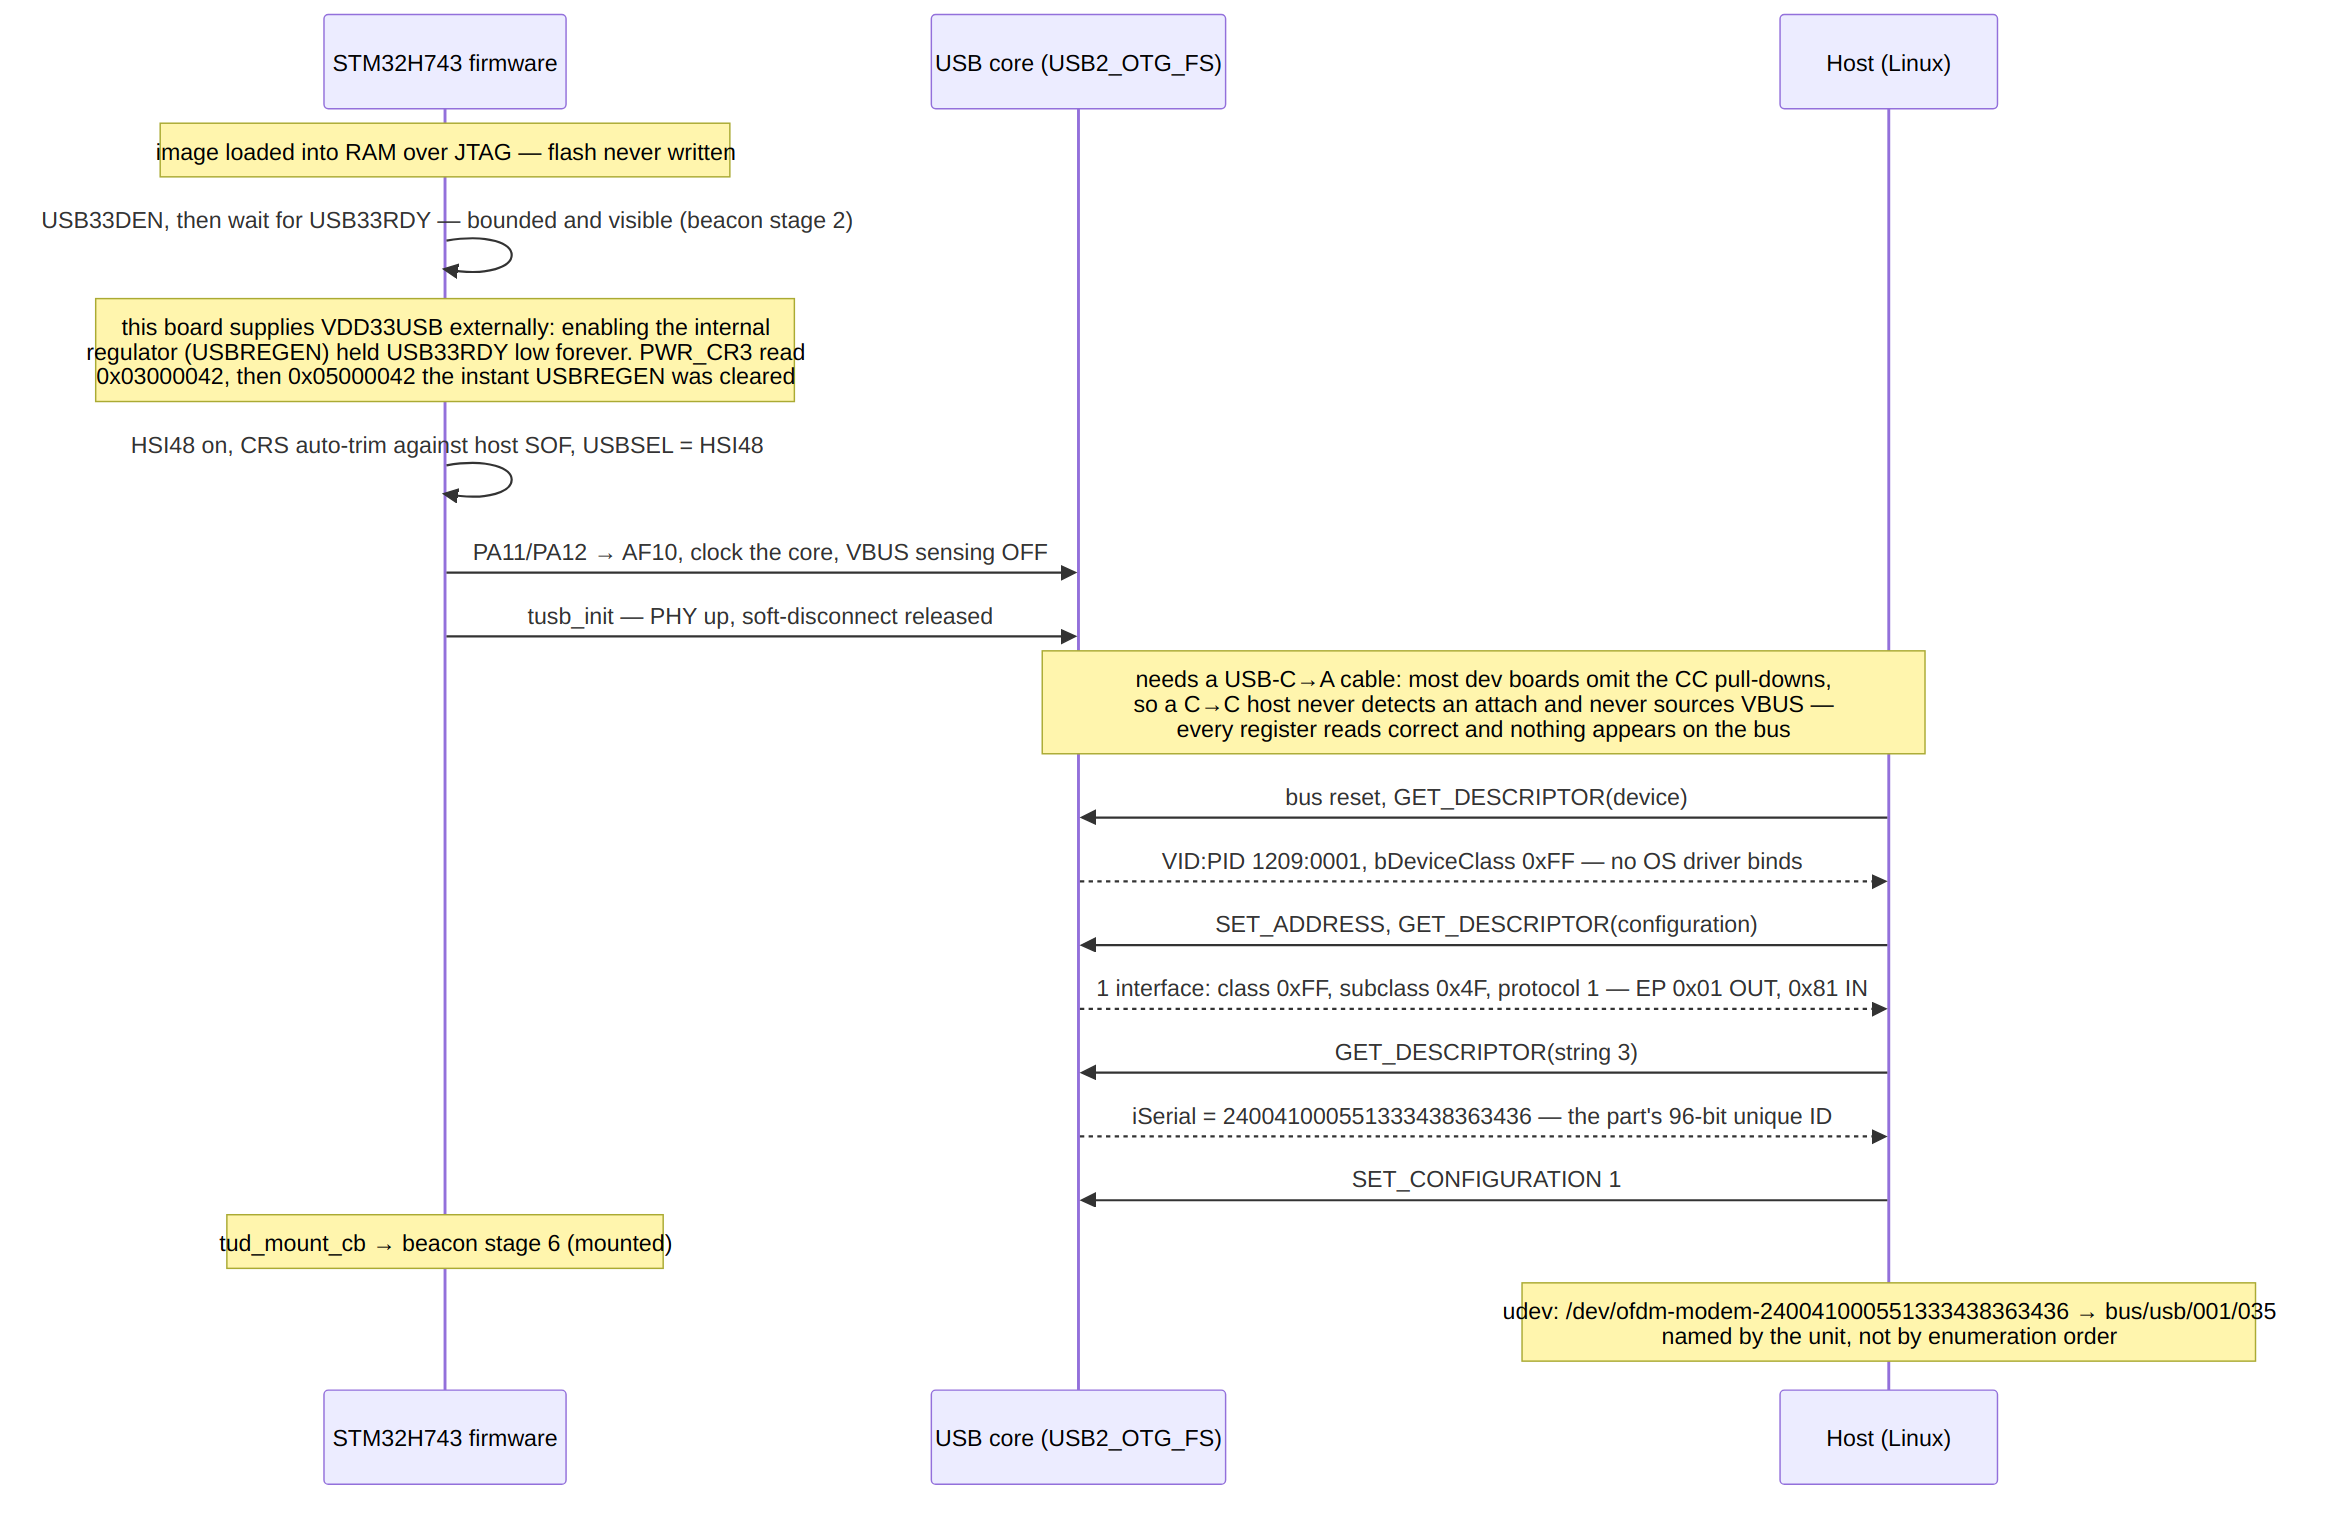
\includegraphics[width=0.92\textwidth]{images/usb_enum_seq.png}
    \caption{Enumeration: supply detection, clocks from HSI48 (trimmed
             against the host's SOF, so the firmware is correct whatever
             the board's crystal), and the descriptors that give the
             device its identity.}
    \label{fig:usbenum}
\end{figure}

\paragraph{A session.} Figure~\ref{fig:usbsession} traces a host
session against the real link layer: the station's queues, rate ladder
and reply timers run for real behind the endpoints, with a stub PHY that
accounts air time and transmits nothing --- the honest shape of a modem
with its antenna disconnected. Status is pushed unprompted twice a
second whenever the device is mounted; the diagnostic event stream is
opt-in and yields to everything else, because a lost diagnostic costs
nothing and a lost reply costs the session.

\begin{figure}[htbp]
    \centering
    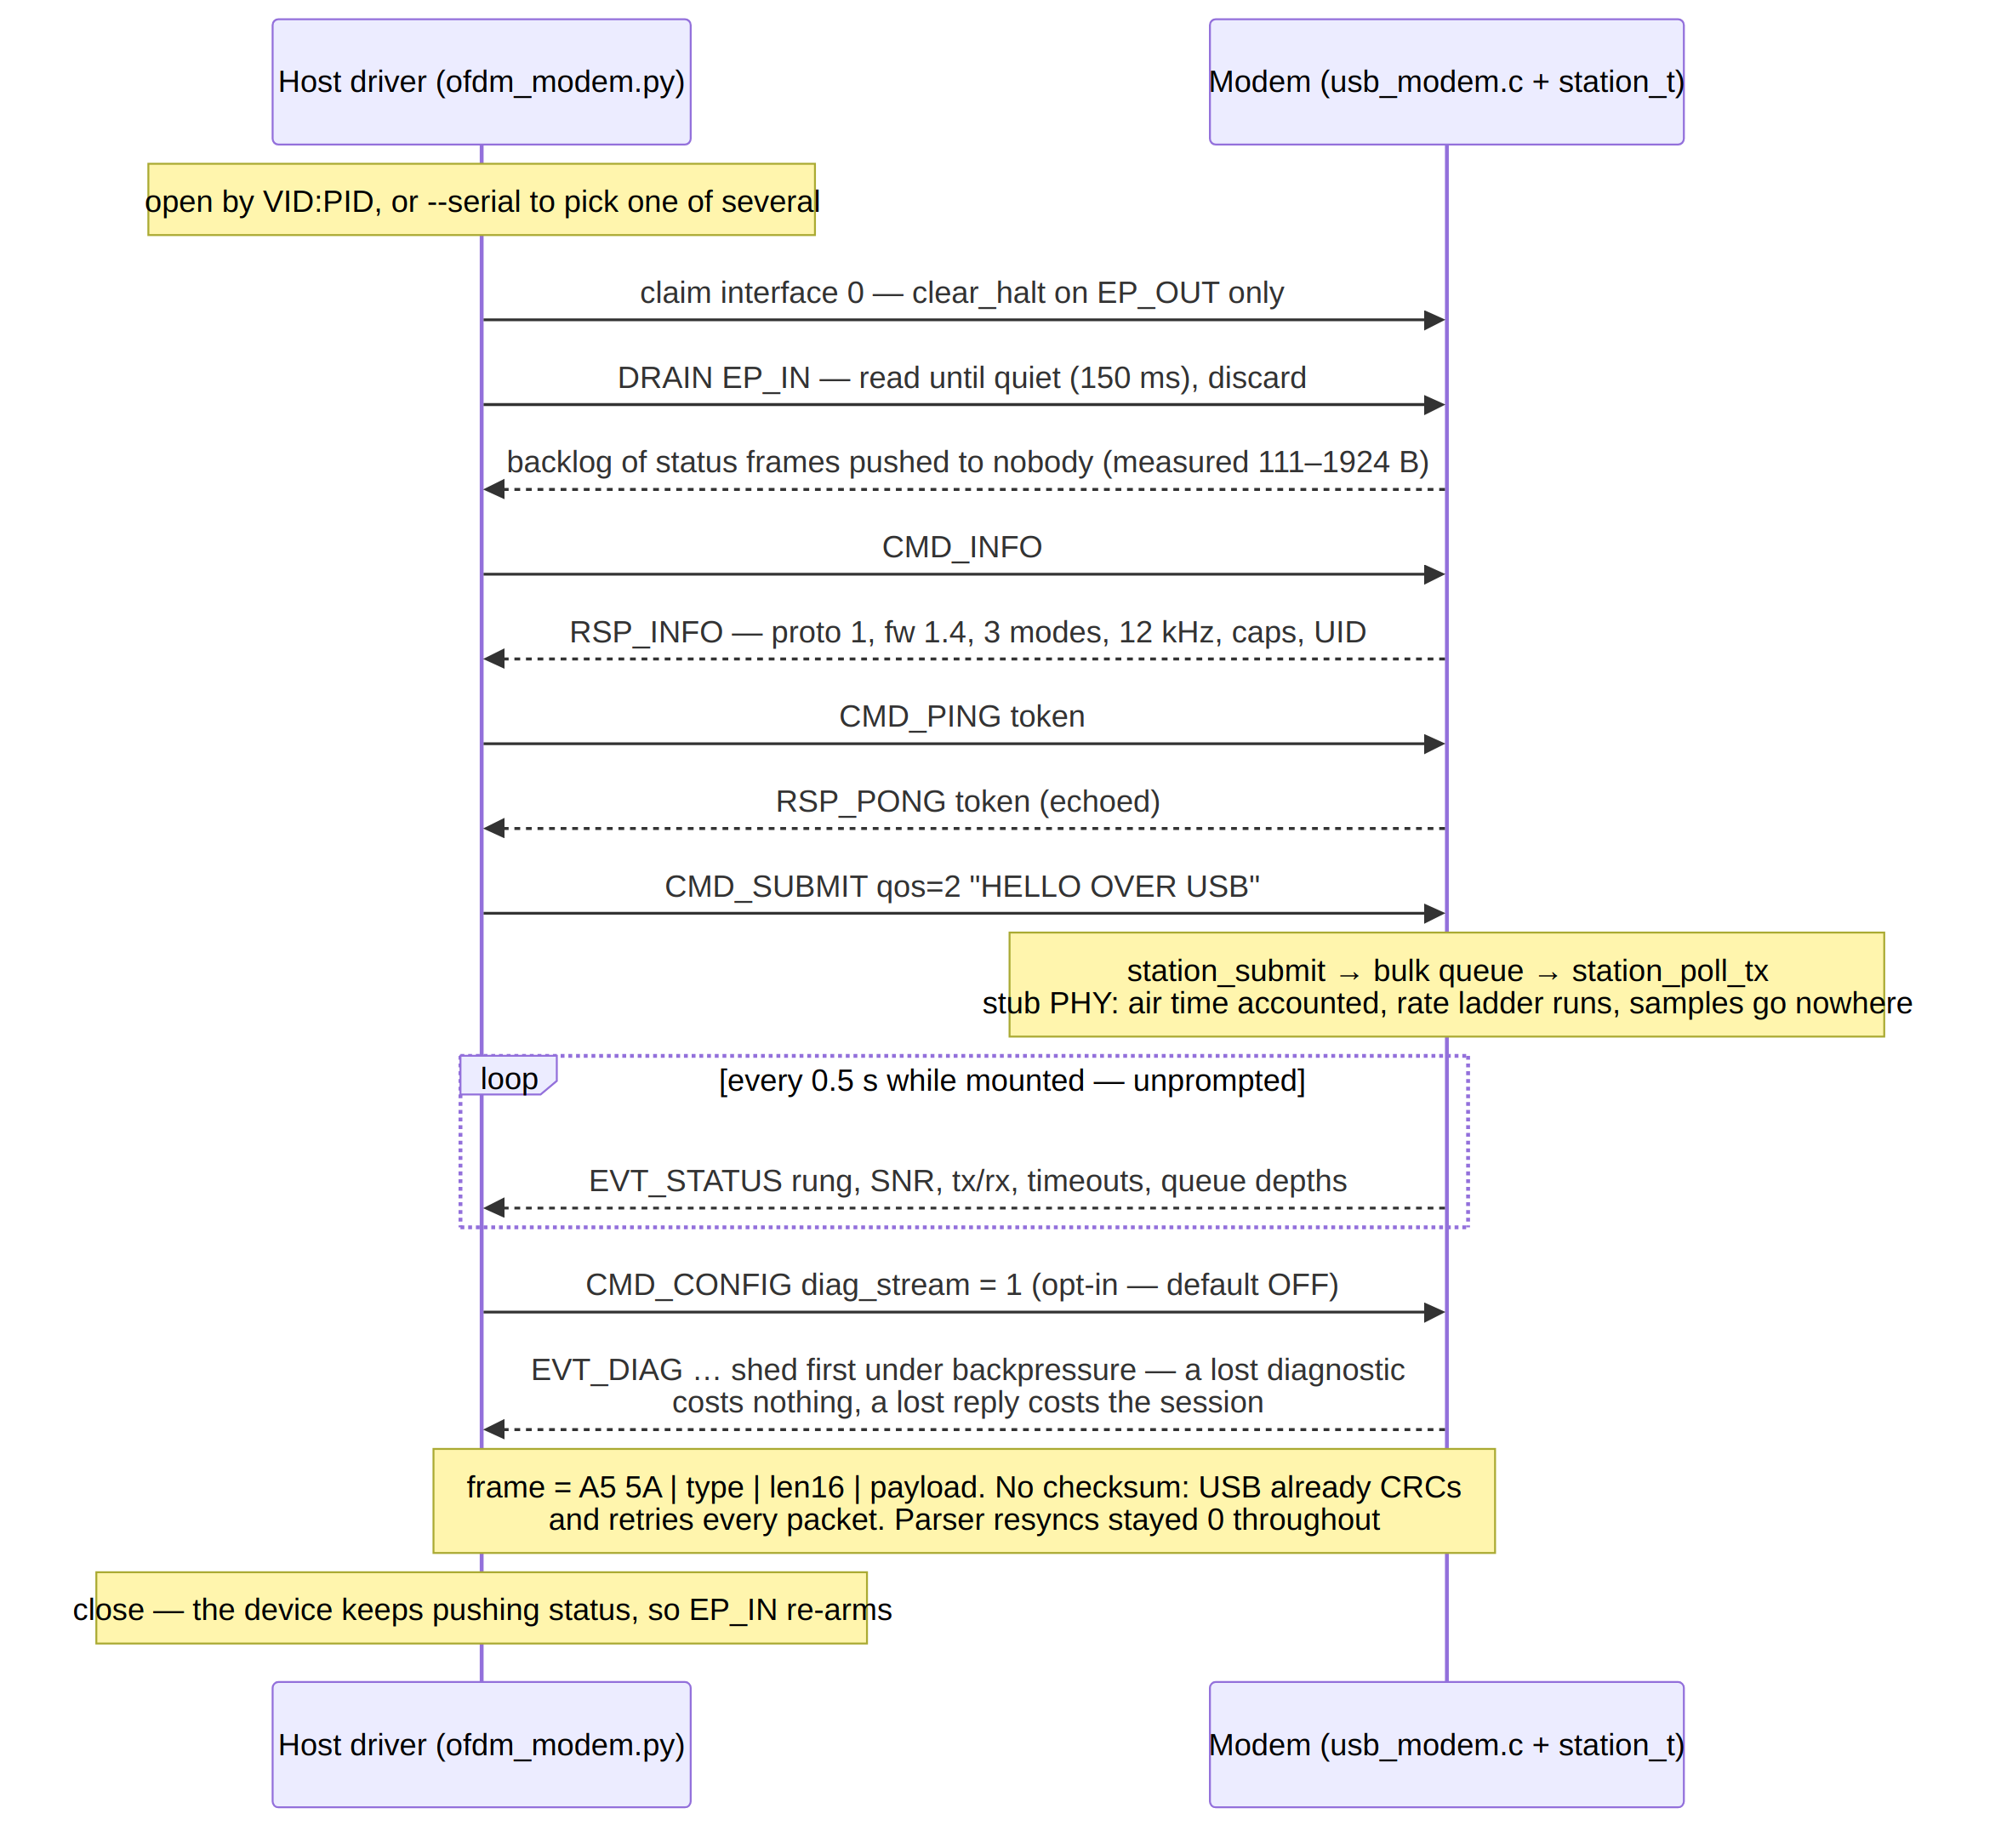
\includegraphics[width=0.92\textwidth]{images/usb_session_seq.png}
    \caption{A host session: open, drain, identify, command and reply,
             unprompted status, opt-in diagnostics.}
    \label{fig:usbsession}
\end{figure}

\paragraph{The wedge, and why the host must drain rather than reset.}
The station image enumerated correctly and then, for most of a day,
answered nothing and fell silent after a single packet --- deterministically,
across four builds. Five hypotheses were disproven by measurement
(a diagnostic firehose, loop starvation under polling, cache against
DMA, polling against interrupts, the clock), and three unrelated bugs
fixed on the way, before the instrumentation at the moment of the stall
read: staging queue empty, 150 bytes free of a 512-byte TinyUSB transmit
FIFO, 399 bytes handed over. That is 362 bytes sitting \emph{inside}
TinyUSB unsent --- 29 (the \texttt{RSP\_INFO} reply) plus nine 37-byte
status frames, exactly --- and $399-362=37$: precisely one frame ever
reached the wire. The device was not silent; it was mute.

The cause, confirmed from TinyUSB's source and shown in
Figure~\ref{fig:usbreopen}, is an interaction between an ordinary host
habit and the library's clear-stall handling. Because the device pushes
status unprompted, its IN endpoint is normally \emph{armed} with a frame
when a host opens it. The host driver called \texttt{clear\_halt} on
that endpoint on open --- a common recovery idiom, and one added during
this work. \texttt{usbd\_edpt\_clear\_stall} drops its software BUSY
flag unconditionally (its own comment calls this ``long-standing
behavior''), while the dwc2 \texttt{dcd\_edpt\_clear\_stall} only clears
the STALL bit and resets the PID; nothing disarms the hardware. The next
flush sees ``not busy'' and re-arms the endpoint on top of a live
transfer --- undefined on the core --- so one packet escapes, the
completion no longer matches what the library started, and BUSY never
clears. The level-triggered FIFO-empty interrupt then storms:
\texttt{isr\_count} reached 90 million.

It was confirmed by prediction rather than by fix. Holding status frames
until the host had spoken, so the endpoint was idle at open, made the
\emph{first} open work --- and every later open still wedged, exactly as
the mechanism requires, since by then the device was pushing again.

The fix is on the host: consume the armed transfer instead of resetting
the endpoint. The driver reads the IN endpoint with short timeouts until
it goes quiet and discards what it finds; \texttt{clear\_halt} is kept
for the OUT endpoint only, where three opens against an armed endpoint
measured harmless. The device is unchanged --- pushing status while
mounted is the right thing for a modem to do, and is the case a driver
must handle. Verified on the part: three consecutive opens (draining
1924, 185 and 111 stale bytes) and a session killed mid-read then
reopened (draining 37 bytes: the one frame armed at the kill), all
answering, submitting and reading with zero resynchronisations;
\texttt{isr\_count} 293 against 90 million wedged, no faults, no drops.

\begin{figure}[htbp]
    \centering
    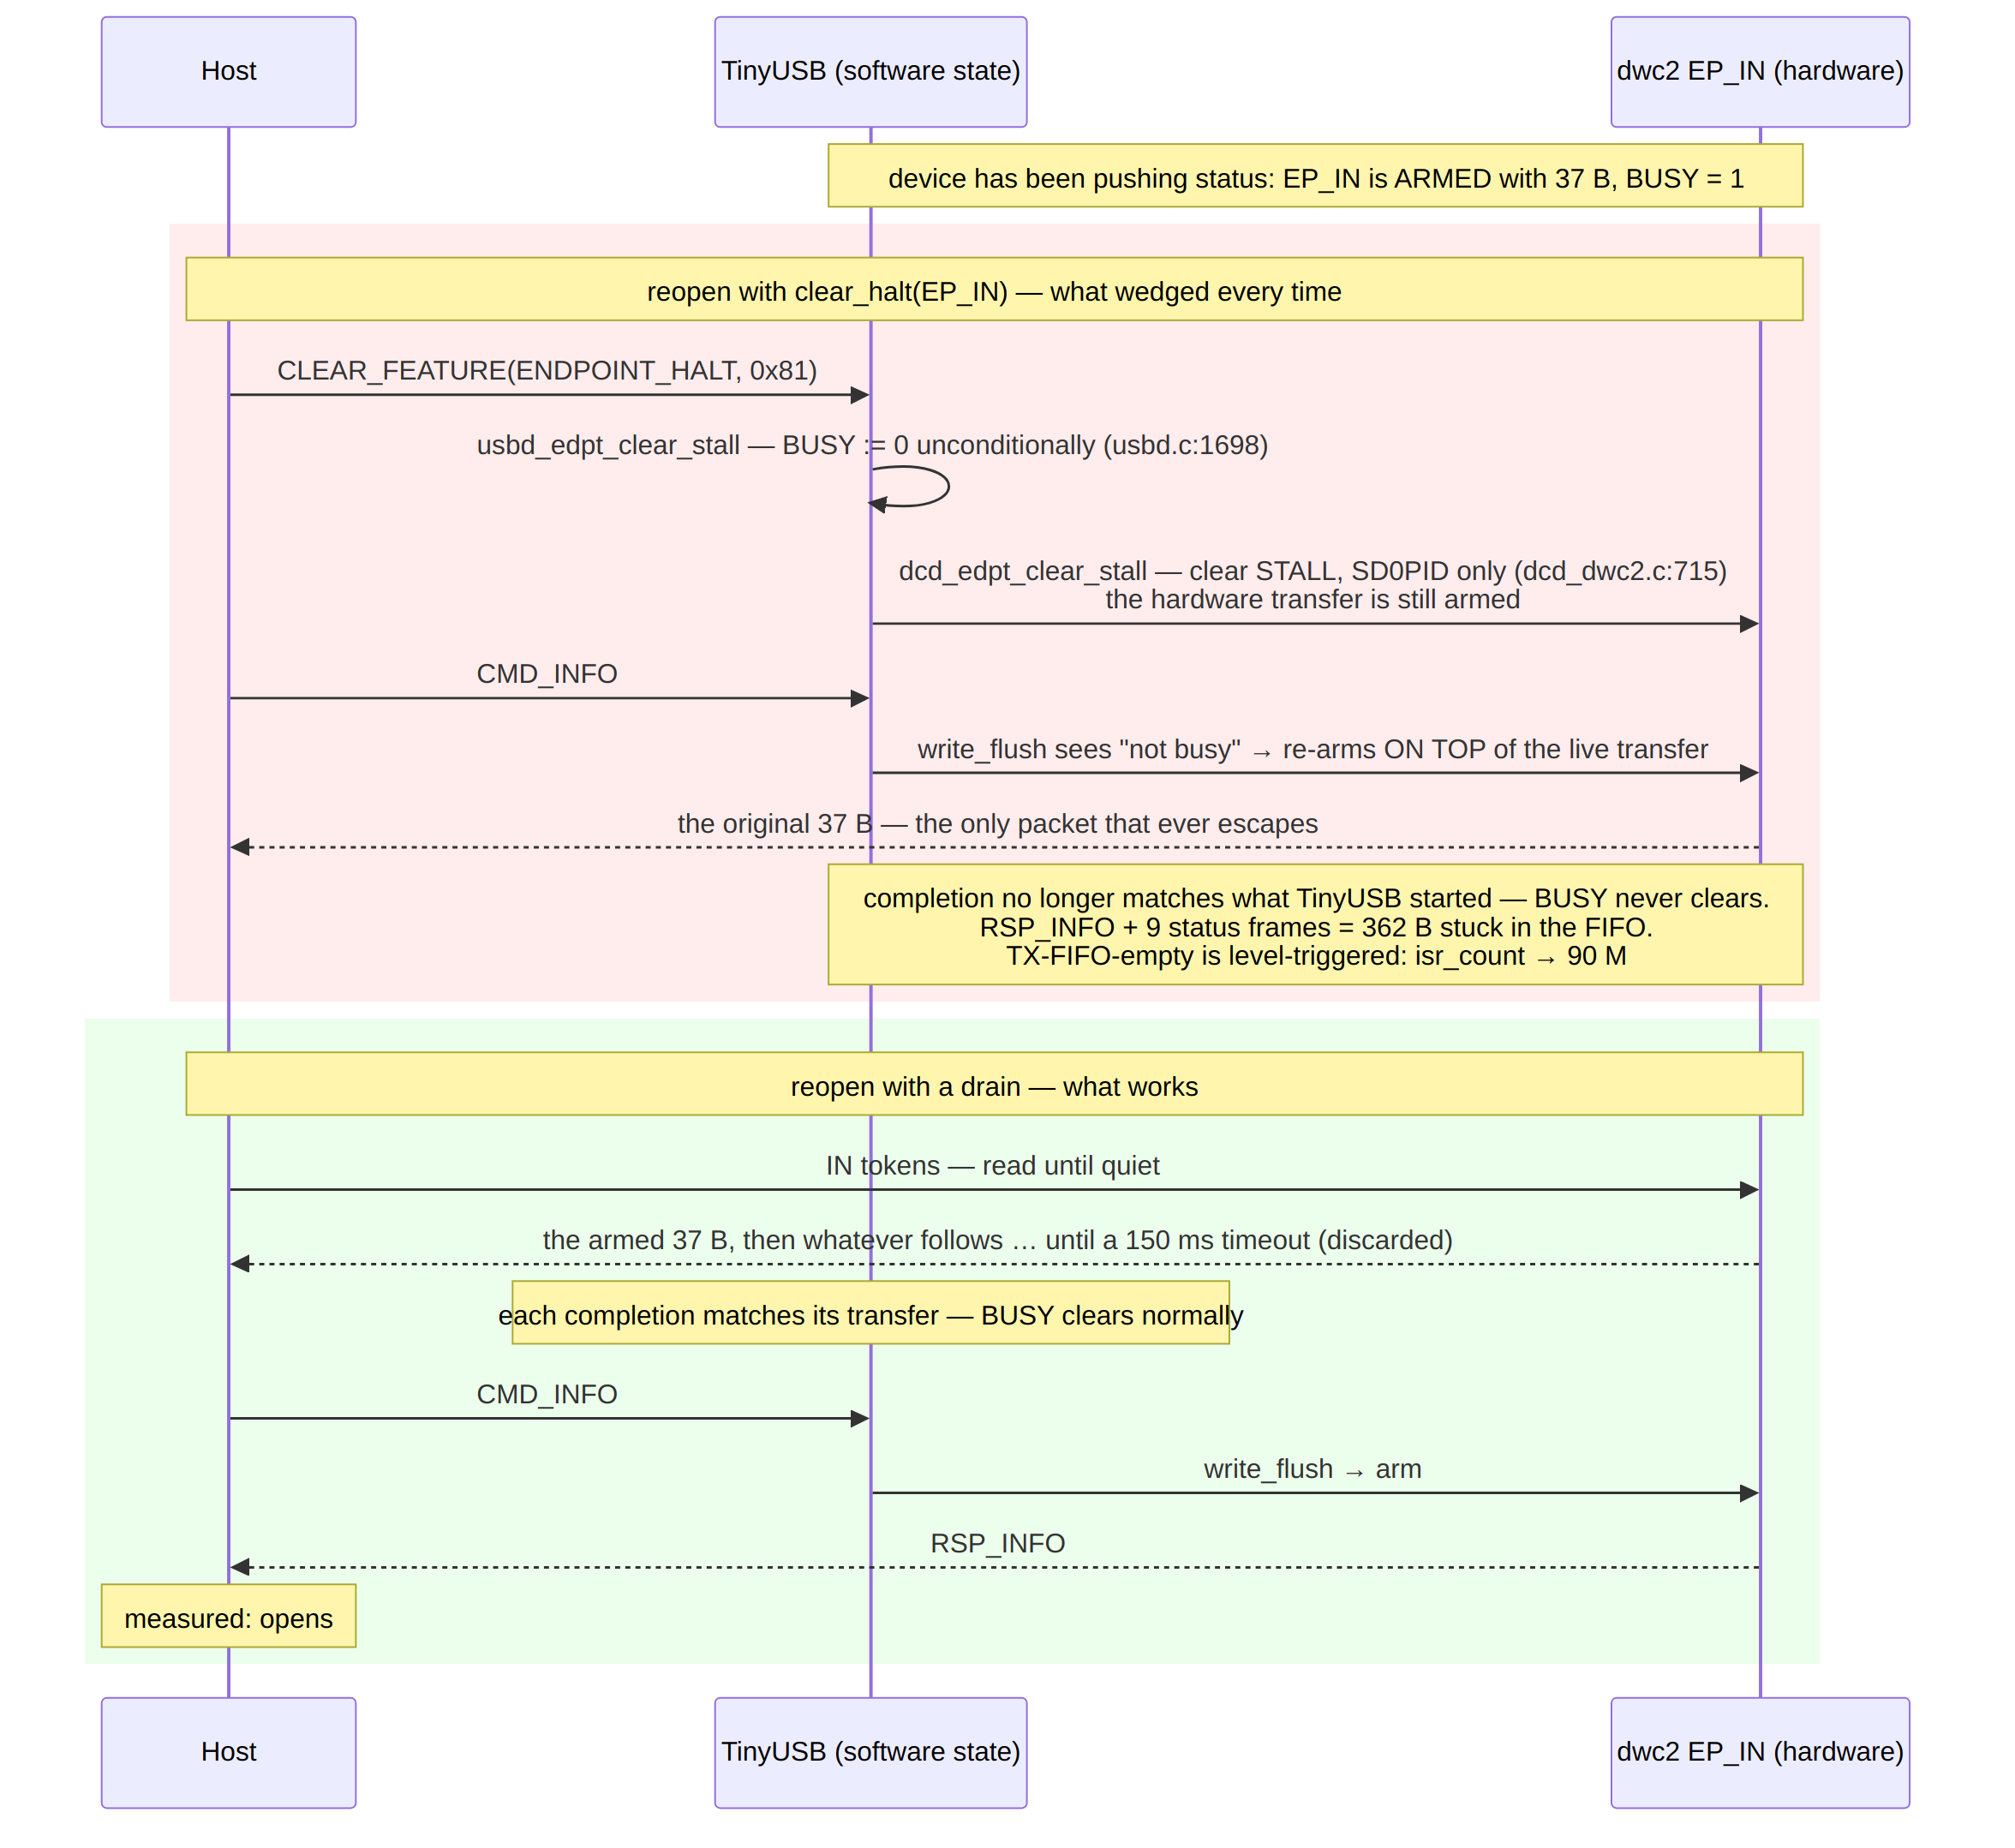
\includegraphics[width=0.92\textwidth]{images/usb_reopen_seq.png}
    \caption{Reopening against a device that is already pushing. Above:
             \texttt{clear\_halt} on an armed IN endpoint desynchronises
             TinyUSB's software state from the hardware and wedges it
             after one packet. Below: draining the endpoint consumes the
             armed transfer through the normal path.}
    \label{fig:usbreopen}
\end{figure}

Two qualifications. VID:PID \texttt{1209:0001} is the pid.codes
\emph{test} identifier, correct for development and wrong for anything
shipped: a released unit needs an allocated product ID, or it collides
with every other prototype using the same one. And the device has not
been made robust to \texttt{clear\_halt} on an armed endpoint itself;
that is TinyUSB's clear-stall path rather than this project's, so the
contract is stated instead --- any client for this device must drain,
not reset.

\subsection{Two Boards on a Wire}
\label{sec:cport_twoboard}

Everything to this point validated the chain against something the
project itself controls: golden vectors, a simulated channel, a virtual
audio daemon, and an SDR whose transmit and receive halves share one
oscillator. One impairment was never exercised by any of them --- two
\emph{independent} clocks. A single-board loopback cannot supply it
either: playing to \texttt{DAC1\_OUT1} and recording \texttt{ADC1} on
the same board runs both converters off one TIM6, so the sample-rate
offset is exactly zero by construction, and the receiver's tolerance to
it is untested no matter how much copper the signal crosses.

The stand in Figure~\ref{fig:twoboardlink} removes that last shared
assumption. Board A's DAC drives board B's ADC through one signal wire
and one ground wire; each board clocks its converter from its own
crystal and its own PLL, and the two never exchange a timing signal ---
not even to start. One ESP32 debugs both boards at once: JTAG
daisy-chains, so \texttt{TDI}/\texttt{TDO} thread through board A into
board B and back to the probe, which costs exactly one wire beyond a
second board's worth of the existing harness. The three push-pull
control lines are duplicated onto a driver pin per board rather than
spliced; because a line and its copy sit in the same GPIO bank, the
firmware switches both in one \texttt{w1ts}/\texttt{w1tc} store, so
there is no skew between the boards at all. That is a wiring
convenience rather than a fix: at the probe's measured 42\,236 edges/s
a TCK half-period is 25\,\textmu s, against nanoseconds of everything
else.

\begin{figure}[htbp]
    \centering
    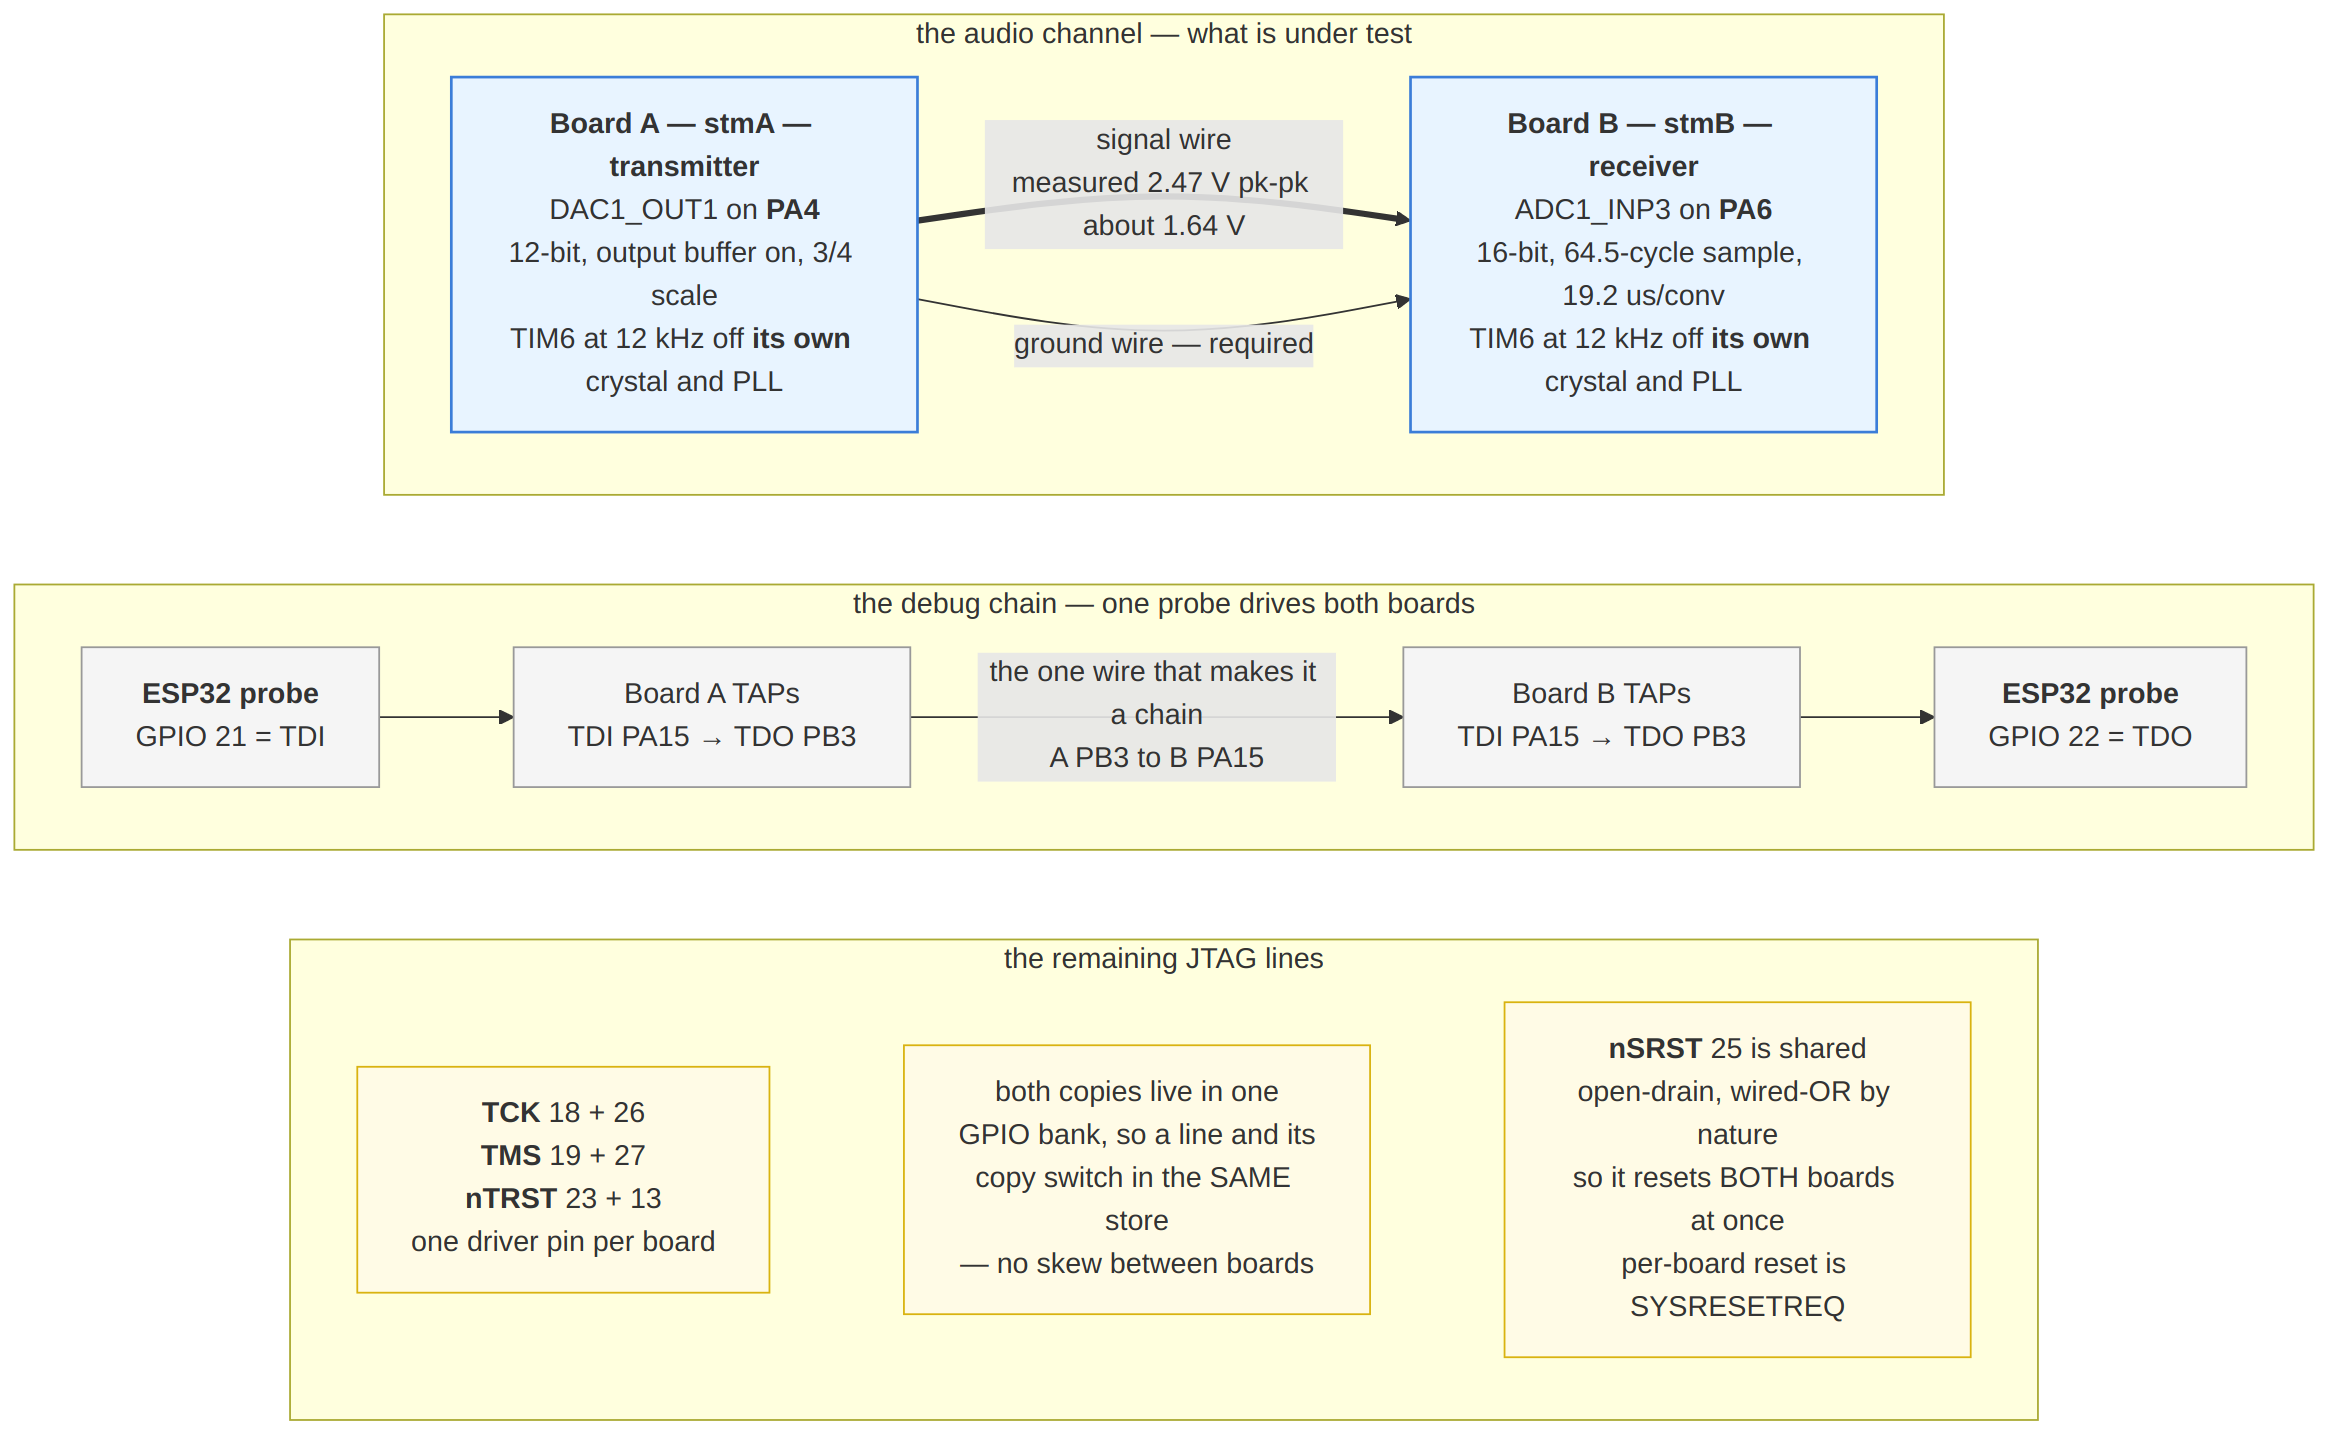
\includegraphics[width=\textwidth]{images/two_board_link.png}
    \caption{The two-board stand. The audio channel is one signal wire
             and one ground wire between converters that share no clock;
             the debug chain is a single probe threaded through both
             boards' TAPs. \texttt{nSRST} is deliberately not
             duplicated --- it is open-drain and wired-OR by nature, and
             duplicating it would not buy per-board reset anyway, since
             \texttt{remote\_bitbang} drives both resets from one pair of
             commands.}
    \label{fig:twoboardlink}
\end{figure}

One image serves both roles, selected over JTAG before the CPU is
released, because a station is half duplex and its transmitter shares
the receiver's arena --- no board ever does both. The transmitter builds
one NORMAL QPSK frame and replays it; the receiver records 54\,000
samples and only then runs the streaming receiver over the recording, so
the analog path can be characterised independently of whether the
decoder liked it. The host releases the transmitter \emph{first}, which
is what removes the need for a trigger: the whole capture window falls
inside a transmission already in progress.

\begin{table}[H]
    \centering
    \caption{Two boards, one wire, independent clocks. Measured on the
             stand; the payload check is \texttt{memcmp} against the
             transmitted packet, so ``bit-exact'' is exact.}
    \label{tab:twoboard}
    \small
    \begin{tabular}{@{}lll@{}}
    \toprule
    \textbf{Quantity} & \textbf{Measured} & \textbf{Note} \\
    \midrule
    Complete frames in window & 2 & 54\,000 samples at 12\,kHz \\
    Decoded bit-exact         & \textbf{2 of 2} & \texttt{memcmp} vs.\ the
                                                  transmitted packet \\
    ADC swing                 & 2.472\,V pk-pk & about 1.643\,V, the
                                                 DAC's mid-rail \\
    Residual CFO              & $+0.01$\,Hz & after preamble correction \\
    ADC conversion            & 19.2\,\textmu s & 64.5-cycle sample,
                                                  \texttt{per\_ck}/8 \\
    Receiver ISR              & 19.5\,\textmu s & of an 83.3\,\textmu s
                                                  period, i.e.\ 23\,\% \\
    Transmitter ISR           & 0.11\,\textmu s & one DAC store \\
    \bottomrule
    \end{tabular}
\end{table}

\paragraph{What it corrected: a vector table in cached SRAM.} The
receiver role hung on its first run --- stage ``running'', its TIM6
interrupt count stuck at zero, the run loop spinning until the
three-minute timeout. The state read off the part was contradictory:
TIM6 counting with its update flag set, the interrupt \emph{pending}
(\texttt{ISPR1}~$=$~\texttt{0x400000}) but \emph{not enabled}
(\texttt{ISER1}~$=$~0), \texttt{PRIMASK} clear --- and the vector table
in memory holding the correct handler. The status block explained the
disable: the first interrupt had been taken by the \emph{stray} handler,
whose job is to mask an unexpected source rather than let it wedge the
device, so it had cleared the enable for IRQ~54.

The vector table lives in ordinary cached SRAM, and
\texttt{vectors\_set()} wrote the entry and executed \texttt{DSB} ---
which orders accesses but does not clean. On a Cortex-M7 an exception
vector fetch reads \emph{memory}, not the D-cache, so the new entry sat
in a dirty line while the hardware still fetched the old one. Reading
the table over JTAG showed the correct handler only because the line had
been evicted by then, which is precisely what made the failure look
impossible. \texttt{SCB\_CCR} read \texttt{0x00070200} on the stalled
board, \texttt{DC} set --- inherited from the USB firmware the RAM image
had displaced. The transmitter role never hit it because
\texttt{build\_frame()} runs between installing the handler and the
first interrupt and evicts the line in time: the same binary on the same
board, differing only in eviction timing, which is why the bug presented
as role-dependent. Both entry points now clean by MVA. This had been
latent under every RAM bench in the project.

Two smaller hazards came from the same root --- a RAM image inherits the
machine state of the firmware it replaced. \texttt{ISER3} bit~5
(\texttt{OTG\_FS}) is still set when the image starts, so an inherited
enable can deliver a stale interrupt as the first one and get its source
masked; \texttt{vectors\_irq\_enable()} therefore clears the pending bit
before setting the enable, and the bench masks interrupts for the whole
of bring-up.

\paragraph{What was not measured.} The obvious way to report the
sample-rate offset --- compare the two boards' measured TIM6 clocks ---
is structurally incapable of showing it, and would have produced a
confident \emph{0.0\,ppm}. Each board measures TIM6 against its own DWT
cycle counter, and both are derived from the \emph{same} PLL, so that
ratio is exact on each board and identical between them however far
apart the crystals are. The offset is instead read off the wire, from
the spacing of consecutively decoded frames against the number of
samples transmitted between them. With only two complete frames in the
capture window the span is 17\,920 samples, and a start position good to
one sample makes that a \emph{bound} rather than a figure: the two
clocks agree to within $\pm$56\,ppm. That is consistent with the
$+0.01$\,Hz residual CFO, and it is enough to say the link decodes
across independent clocks --- but it is not a measurement of their
offset. A tighter number needs a much longer capture, which needs the
receiver to decode as it goes rather than into a buffer; that is the
next step for this stand, not a result of it.

\subsection{A Board That Is a Radio}
\label{sec:cport_radio}

Section~\ref{sec:cport_usb} gave the board an identity and a host
protocol, but bound the station to a \emph{stub} PHY: queues, rate
ladder, ARQ and reply timers all ran for real, and nothing reached the
air. Section~\ref{sec:cport_twoboard} gave the opposite half --- frames
crossing copper between two boards' converters --- with no link layer
above them and no host beside them. This section is the two in one
image: a board a host drives over USB and a peer hears over a wire.

\begin{figure}[htbp]
    \centering
    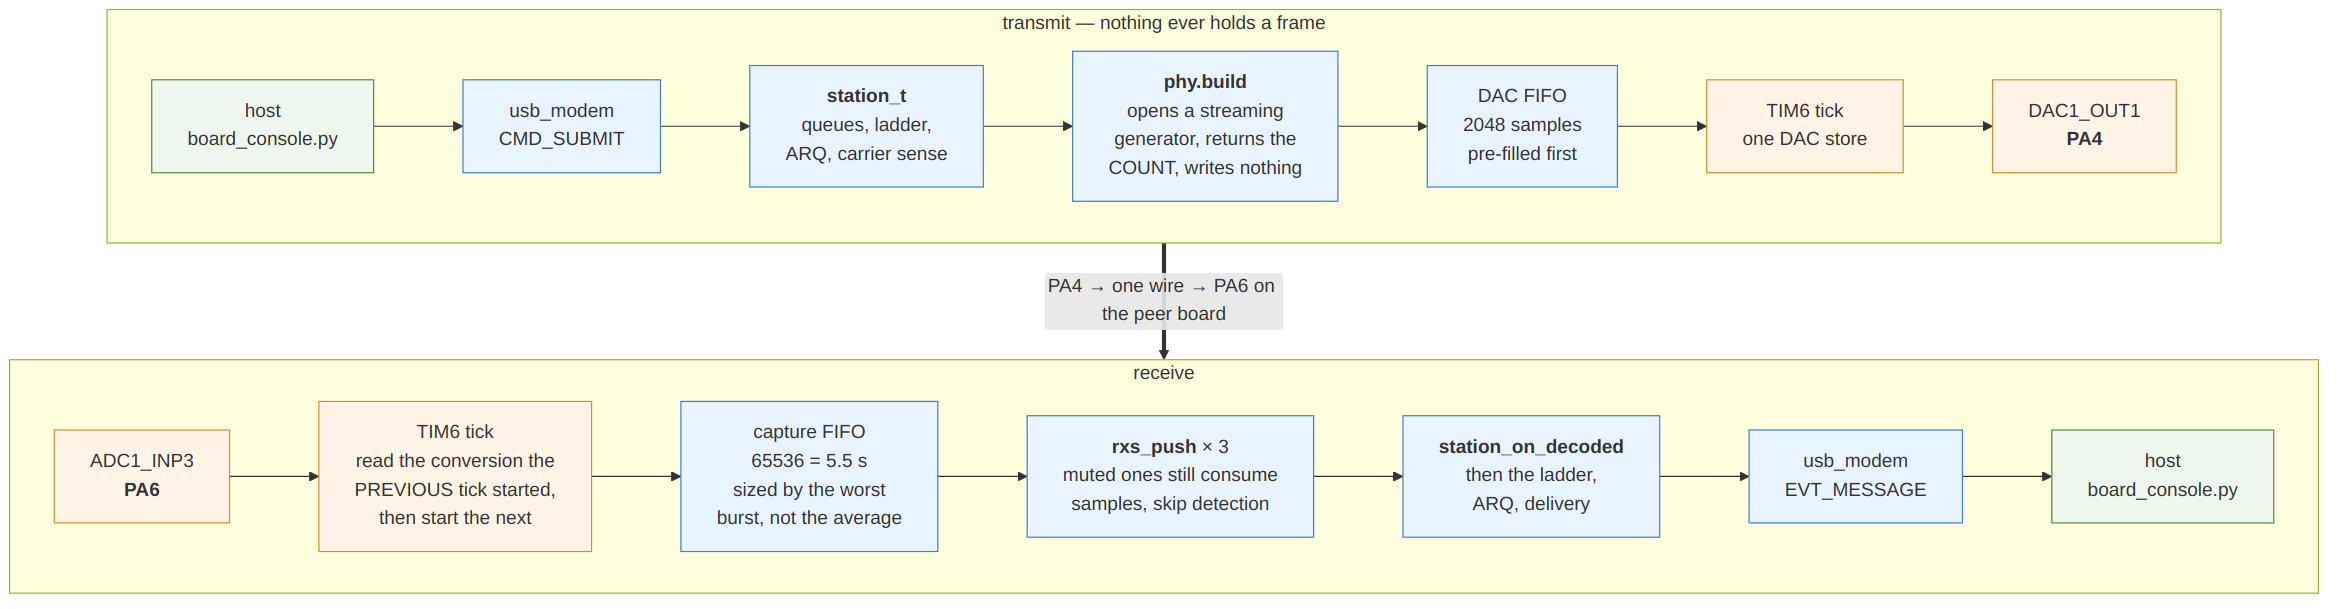
\includegraphics[width=\textwidth]{images/radio_firmware.png}
    \caption{The radio firmware. Half duplex here is a contract rather
             than a simplification: the streaming generator's state
             lives in the shared arena \emph{across} \texttt{txs\_pull}
             calls while the receiver's scratch is call-scoped, so
             \texttt{rxs\_push} must never run during a transmission ---
             and does not, because the tick feeds only one FIFO at a
             time.}
    \label{fig:radiofw}
\end{figure}

\paragraph{The transmitter never renders a frame.}
\texttt{station\_phy\_t::build} is frame-at-once: it is handed a buffer
and returns a sample count. An EXTREME frame is about 456\,000 samples
--- 912\,kB --- which this part cannot hold, and demoapp's answer (a
600\,000-sample buffer) is not available. It is also unnecessary. The
station never reads or writes those samples: \texttt{out} and
\texttt{out\_cap} appear nowhere in \texttt{station\_poll\_tx} except
where they are passed through to \texttt{build}, and the count is what
the caller acts on. So \texttt{build} here opens a \emph{streaming}
generator and returns the total it reports without writing a sample,
and the main loop pulls from that generator into a 2048-sample FIFO as
the tick drains it. The waveform is identical either way --- a one-block
burst with no resync is bit-for-bit a frame, which both test suites
already assert.

The 12\,kHz tick never blocks. The analog bench of
Section~\ref{sec:cport_twoboard} started a conversion and waited for it
inside the tick, 19.2\,\textmu s of an 83.3\,\textmu s period; that was
free when the decoder ran afterwards and is not free when the decoder
has to keep up. Here the tick reads the conversion the \emph{previous}
tick started and immediately starts the next, so the sample is one tick
old --- a constant delay indistinguishable from cable length.

\paragraph{What it corrected: the flash images never enabled the
caches.} The receiving board dropped 1\,522\,686 captured samples ---
64\,\% of everything its ADC produced --- and decoded nothing, while the
transmitting board underran its DAC 375 times. \texttt{SCB\_CCR} read
\texttt{0x00040200} on the running part: both L1 caches off.
\texttt{startup\_flash.c} had never enabled them, so code ran from flash
at two wait states with no instruction cache and every SRAM access
uncached, which is five to ten times slower than the same code out of
ITCM. It had not mattered while the flash images only ran a USB endpoint
and a link layer, and the RAM benches never showed it because their
\texttt{.text} lives in ITCM and needs no cache. Enabling both (the data
cache invalidated by set/way first) cut overruns by 61$\times$. Two
consequences follow and are handled rather than discovered later: a
debugger reading over the AHB-AP does \emph{not} see dirty lines, so the
beacon is cleaned explicitly before each read; and a RAM image that now
inherits \texttt{DC}=1 needs its vector-table writes cleaned, which is
what Section~\ref{sec:cport_twoboard} already had to fix.

Three smaller faults surfaced with it. The flash linker script listed
\texttt{.bss} \emph{before} \texttt{.d2\_bss}, and \texttt{.bss}'s
\texttt{*(.bss*)} matches \texttt{.bss.g\_raw} too --- so the D2 lines
matched nothing, the 160\,kB sample ring sat in AXI, and adding the
receiver overflowed AXI by 100\,kB while D2 stood completely empty
(\texttt{stm32h743\_usb.ld} always had the right order, which is why only
the flash images were affected). \texttt{TIM6\_DAC}, IRQ~54, had no entry
in the vector table: designated initialisers leave every other slot
\texttt{NULL}, so the first tick would have vectored to address zero.
And arming an empty DAC FIFO underran it once per transmission ---
166 underruns across 3 frames, each one a mid-rail sample on the air ---
which pre-filling before starting the carrier reduces to zero.

\paragraph{Sizing the capture FIFO: the worst burst, not the average.}
The decoder's cost is wildly uneven. Quiet blocks are cheap; the commit
at the end of a frame --- acquisition, demodulation of every tiled
symbol, Viterbi --- is one long blocking call, measured at 2283\,ms
inside a single \texttt{rxs\_push} against a 19.5\,s frame. As an
average that is about 12\,\% duty, comfortably real time. What matters
is not the average but whether the FIFO can hold the samples that keep
arriving \emph{through} the burst: 16\,384 samples (1.37\,s) could not,
dropping 33\,036 samples mid-frame and decoding nothing, while 65\,536
(5.5\,s) decodes with no overruns at all. The beacon carries
\texttt{cap\_overruns} and \texttt{push\_ms\_max} so this is checked on
the part rather than reasoned about.

\paragraph{The receiver follows the negotiated rung.} Each open receiver
runs its own detector over every sample and the EXTREME one is much the
most expensive; three concurrently do not fit real time on this part.
They cannot simply be opened selectively either, because every instance
shares one raw sample ring and indexes it by its \emph{own} sample
counter --- feed a subset and they write each other's history at the
wrong offsets. So all three are opened and the unwanted ones are
\emph{muted}: a muted instance still consumes every sample, keeping the
ring and its own timeline coherent, and skips only the per-block
detection, which is where the cost is. Unmuting rearms the search rather
than resuming, since a state machine that was mid-frame when it went
quiet would otherwise decode a frame whose middle it never saw.

Which are active follows \texttt{ladder\_mode(ctl.my\_req)} --- the rung
\emph{this} station asked the peer to transmit at --- plus two others
that are not optional. EXTREME always, because it is rung~0 and
therefore the bootstrap, it is where the ladder decays to after a spell
of silence, and it is what a peer that cannot hear us falls back to;
muting it would make the link undiscoverable and unrecoverable exactly
when recovery is needed. And the mode last decoded on, because
\texttt{my\_req} is a request rather than an observation: between raising
it and the peer acting on it, the peer is still transmitting at the old
mode, and dropping that mode immediately would make the station deaf for
precisely the exchange that would have confirmed the change --- timeout,
request decays, link oscillates. In the settled bootstrap state, both
terms are EXTREME and exactly one detector runs.

\begin{table}[H]
    \centering
    \caption{Two boards, one wire, driven from two host consoles. Every
             figure read off the boards' beacons or the consoles.}
    \label{tab:radio}
    \small
    \begin{tabular}{@{}lll@{}}
    \toprule
    \textbf{Quantity} & \textbf{Measured} & \textbf{Note} \\
    \midrule
    First message, end to end & 36\,s & EXTREME bootstrap,
                                        $\approx$19.5\,s of air \\
    Second message            & \textbf{15\,s} & after the ladder
                                                 climbed \\
    Frames / decodes, each board & 1 / 1 & B decoded, replied, A decoded
                                           the reply \\
    Capture overruns          & \textbf{0} & both boards, throughout \\
    DAC underruns             & \textbf{0} & both boards, after
                                             pre-filling \\
    Worst single decode       & 2283\,ms & of a 19.5\,s frame,
                                           $\approx$12\,\% duty \\
    Idle listening set        & EXTREME & \texttt{my\_req} 0, one
                                          detector \\
    After the climb           & NORMAL$+$EXTREME & \texttt{my\_req} 9
                                                   (A), 7 (B) \\
    SNR reported              & $+15.0$ / $+9.7$\,dB & A and B \\
    \bottomrule
    \end{tabular}
\end{table}

What this build does not yet do is decode streamed bursts: it provides
\texttt{build\_burst} but leaves \texttt{receive\_burst} \texttt{NULL},
so the station uses per-frame bursts --- which is a supported
configuration rather than a hole, since it is also where the link falls
back when a stream stops delivering. Streamed reception needs
\texttt{rxs\_continue\_burst} driven from the link layer's marker, as
demoapp does.

\subsection{Demonstration Infrastructure}
\label{sec:cport_demo}

The C stack runs end-to-end in an interactive demonstration
(\texttt{demoapp/}): a virtual channel daemon exposes two station
devices and a configuration device over Unix sockets, moves 12\,kHz
\texttt{int16} audio in paced ticks, and applies propagation delay,
AWGN sized against the delivered-signal RMS, one-pole Rayleigh fading,
and half-duplex muting; an optional audio mode plays each station's
receive signal on one stereo channel with the sound card as the pacing
clock, making the protocol audible (the EXTREME bootstrap's 21-second
warble adapting up to sub-second QAM16 chirps).  Two console station
applications (three streaming receivers each, one per mode, over the
shared ring) provide messaging, multi-part file transfer over the
burst protocol, channel statistics, the diagnostic event stream, and
the oscillator fine-tune command.  A scripted smoke test drives the
whole stack --- text plus a 5\,000-byte file across the impaired
channel, byte-compared on arrival --- at $25\times$ time scale; the
protocol clocks itself from received samples, so behaviour is
identical at any scale.  The stop-and-wait inefficiency, the burst
protocol's window bugs, the carrier-sense threshold and the rung-0
fallback were all found by this infrastructure rather than by
inspection.

Figure~\ref{fig:sendfileseq} traces a file transfer through it.  Two
decisions in that sequence are worth isolating.

The file is deflated \emph{whole} before being split into parts, not
per part: a 14162-byte configuration file becomes 5015 bytes on air
($2.82\times$), and compressing each 3\,kB part separately would throw
most of that away.  Compression lives in the application rather than in
\texttt{cport/}, which keeps the C port dependency-free --- an MCU
build swaps zlib for miniz or heatshrink and the wire format is plain
\textsc{deflate} either way.

The transfer also \emph{negotiates before it commits}.  The transmit
rung decays by one step per 90\,s of peer silence
(Section~\ref{sec:link}), so a transfer started after a quiet
spell would otherwise open at a rung the link has never been tested at:
measured, a 37.0\,s frame at rung~4 immediately before the next
exchange settled at rung~12 and 5.1\,s.  A sub-second control frame is
answered, and an answered frame is what moves the ladder, so the probe
goes first and the bulk queue follows behind it.  The staleness test
must ask whether the peer has \emph{ever} reported rather than
subtracting from the initial timestamp --- the sentinel is
$-10^{9}$, and doing the arithmetic anyway reported that the peer had
last been heard from 1000000058\,seconds ago.  It is the same rule the
link layer already follows for sequence numbers, where every value
0--7 is legitimate and ``nothing yet'' must be its own state.

\begin{figure}[H]
    \centering
    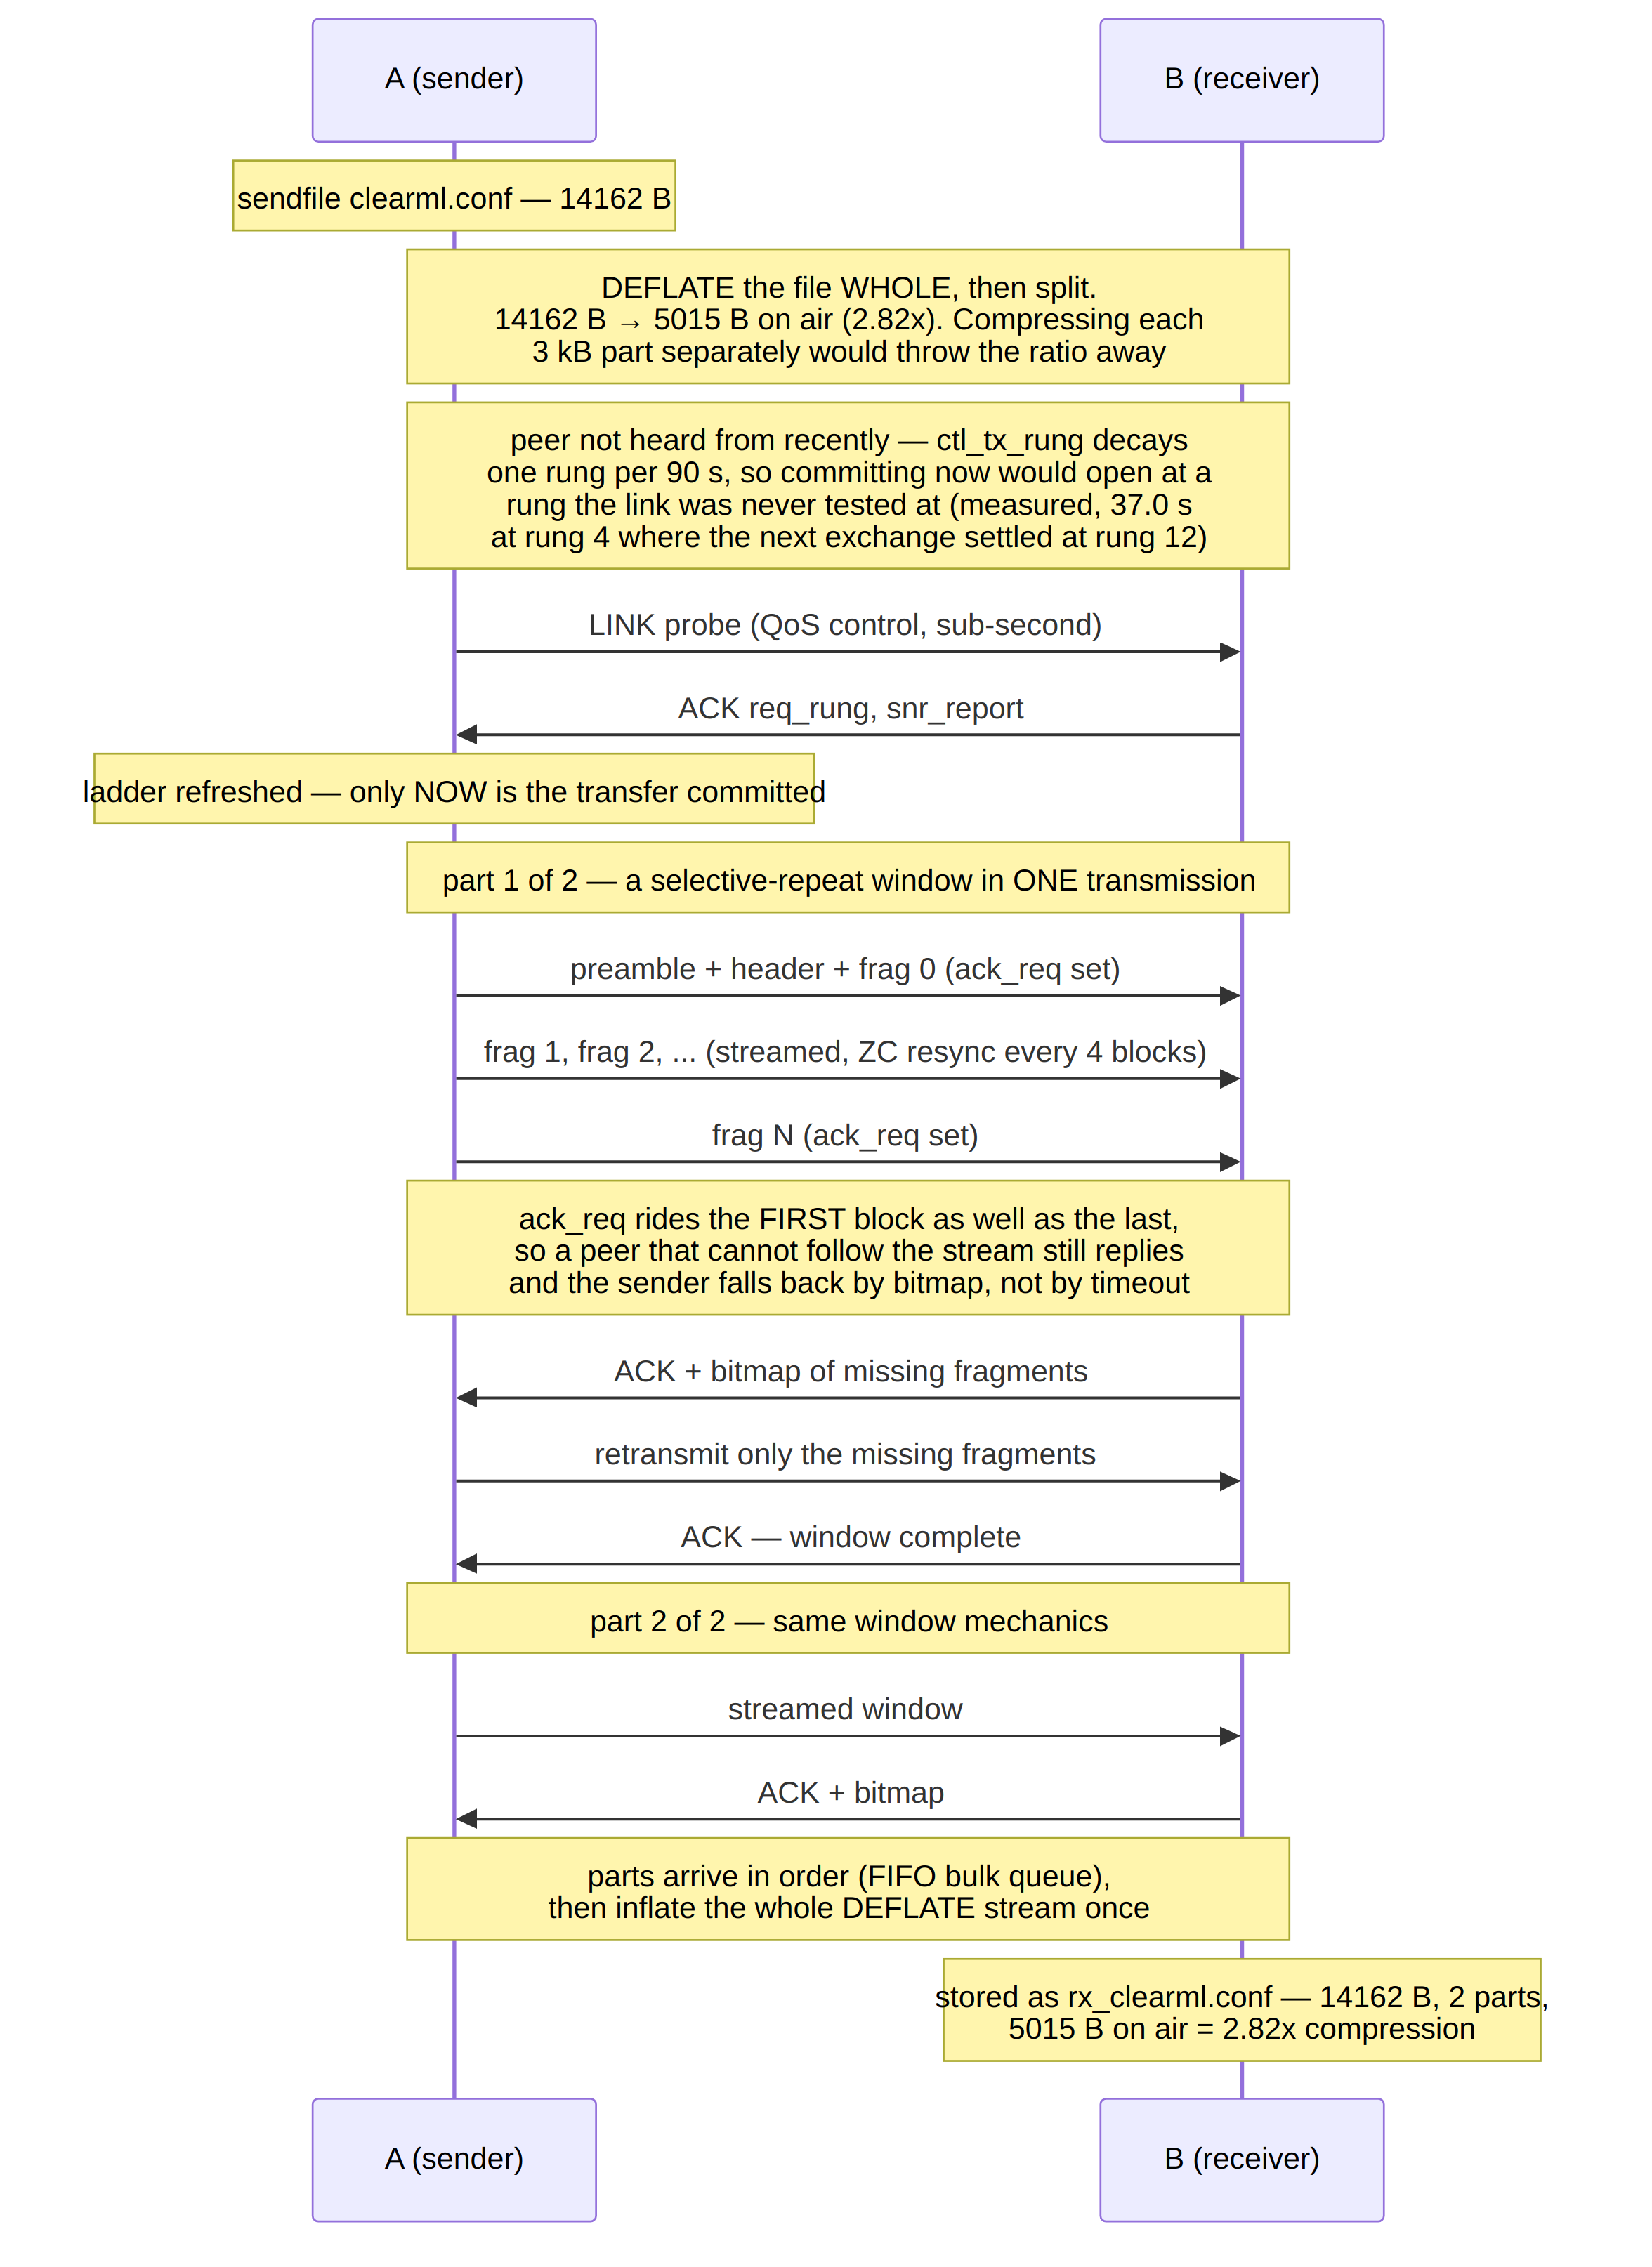
\includegraphics[width=0.90\textwidth]{images/sendfile_seq.png}
    \caption{A file transfer: whole-file compression, a link probe
             before the transfer is committed, then selective-repeat
             windows carried one per transmission.}
    \label{fig:sendfileseq}
\end{figure}

\subsection{From Simulation to a Radio}
\label{sec:cport_sdr}

The demonstration apps talk to a \emph{driver} over a socket rather than
to hardware, which turns out to be the right seam for real radio: an SDR
driver (\texttt{demoapp/sdr\_driver.py}) presenting the same devices puts
the entire C stack on the air with nothing in \texttt{cport/} changed.
It reproduces the SSB model of Section~\ref{sec:rf} sample by sample ---
audio $\rightarrow$ analytic signal (the receiver's own 63-tap Hilbert
design) $\rightarrow$ interpolation to the SDR rate $\rightarrow$ I/Q,
and back, where taking the real part of the decimated baseband
\emph{is} a product detector.  Tuning the radio to the suppressed
carrier makes the two stations' LO error appear as exactly the
audio-band CFO the modem already tracks.  The DSP costs 4.4\,\% of one
core to transmit and 3.1\,\% to receive per audio-second at 2.4\,Msps,
so a laptop runs it comfortably in real time.

Figure~\ref{fig:sdr_setup_loopback} shows the arrangement that needs no
radio at all: the driver cross-connects two stations through the entire
SSB chain --- Hilbert transform, interpolation, int8 quantisation,
decimation and product detection --- so every line of the signal path is
exercised, and the console apps above it cannot tell the difference.
That is what the regression test uses.

\begin{figure}[H]
    \centering
    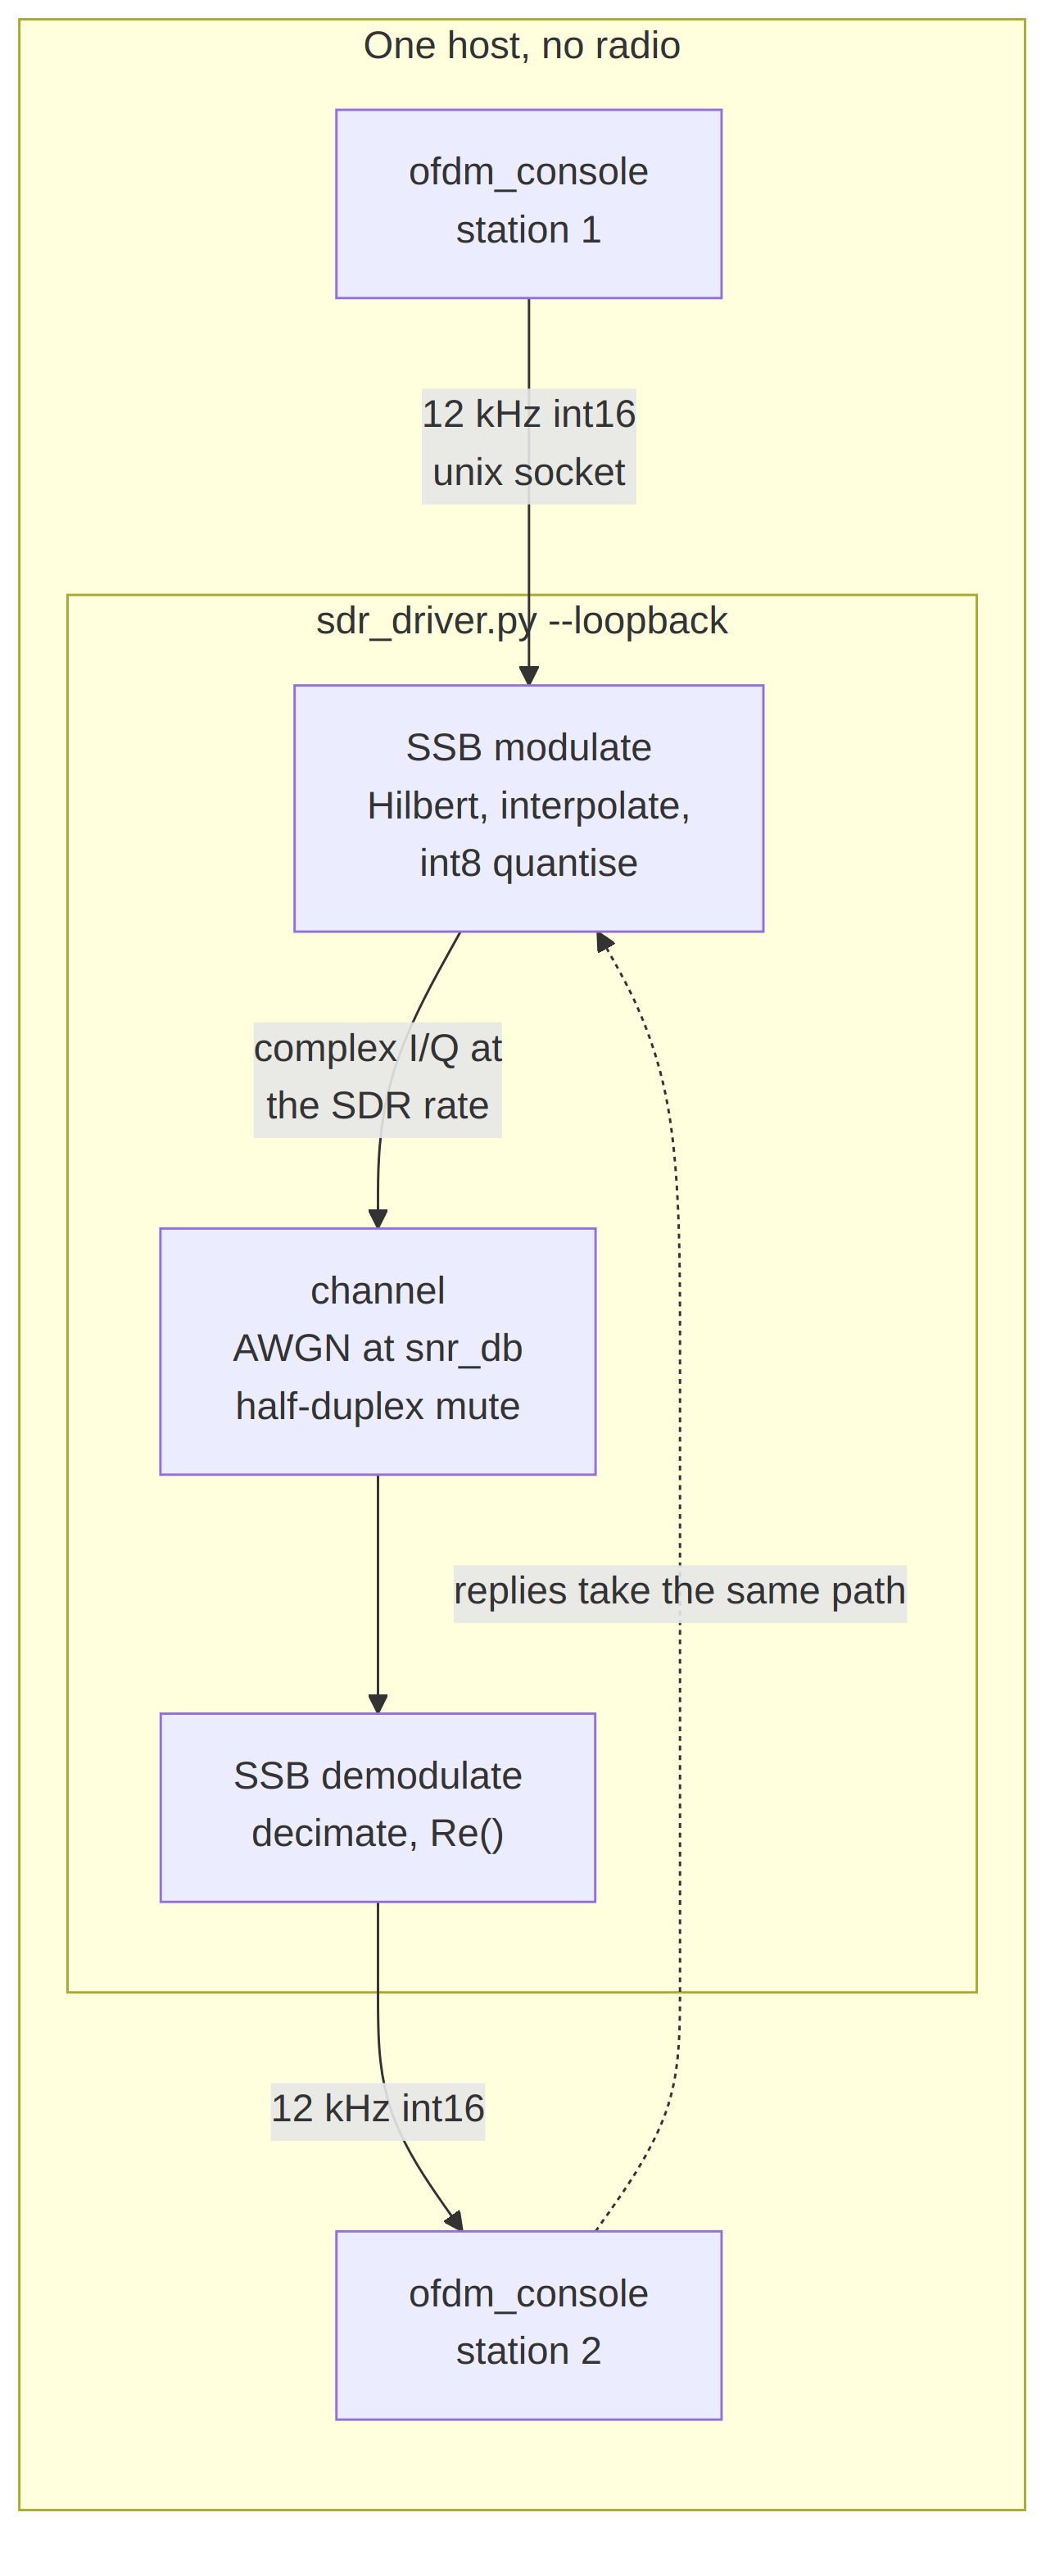
\includegraphics[width=\textwidth]{images/sdr_setup_loopback.png}
    \caption{Hardware-free loopback: two stations cross-connected
             through the full SSB modulation and demodulation chain.}
    \label{fig:sdr_setup_loopback}
\end{figure}

Bringing this up on a HackRF One produced four corrections that no
amount of loopback testing would have found: the local oscillator must
be \emph{offset tuned} (with it on the carrier, the DC leakage lands
inside the 3.5\,kHz passband and the recovered audio was 98\,\% DC ---
the device has neither hardware DC correction nor AGC); the aggregate
gain control is inert and the LNA/VGA/AMP stages must be driven
individually (worth 32\,dB of working level); \texttt{writeStream} only
\emph{queues} samples, so switching back to receive when it returns
truncated the tail of every frame; and a killed process left the radio
\emph{keyed} until a receive stream was opened.

\subsubsection{Instrumented Measurements}

The two measurements that follow share the arrangement of
Figure~\ref{fig:sdr_setup_analyzer}: a tinySA Ultra on USB, used in
both directions.  As an analyser it measures what the radio transmits;
as a source --- through its calibration output, which is a reference
tone at a documented level --- it measures what the receiver makes of a
known input.  Both are scripted, so the numbers below are reproducible
rather than read off a screen.

\begin{figure}[H]
    \centering
    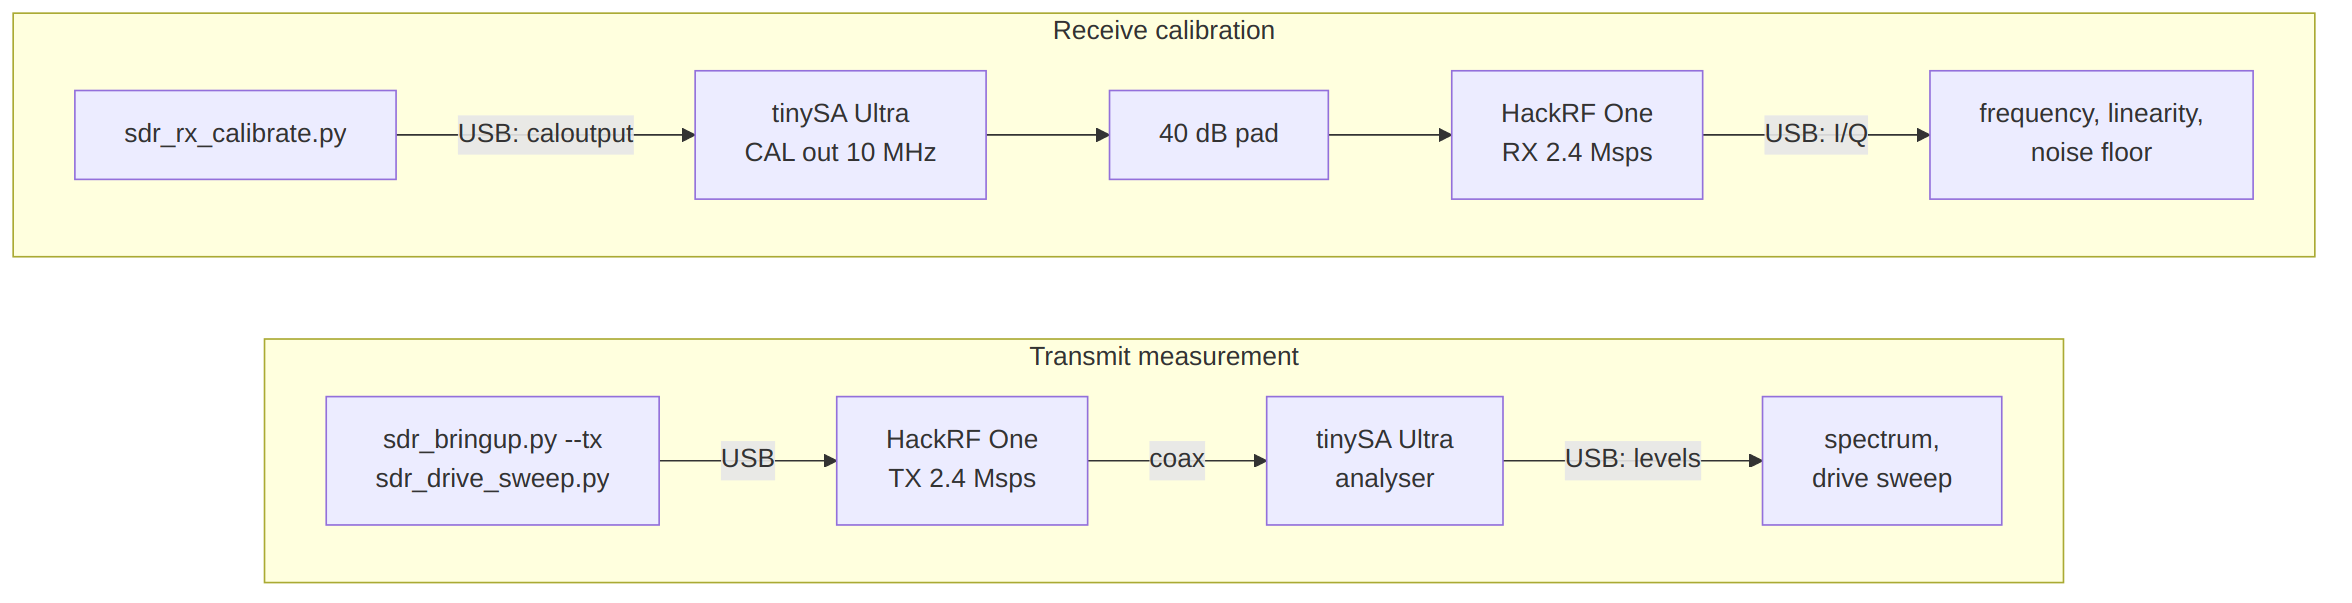
\includegraphics[width=\textwidth]{images/sdr_setup_analyzer.png}
    \caption{Instrumented bench, both directions: as an analyser the
             tinySA measures what the radio transmits; as a source its
             calibration output drives the receiver through a 40\,dB
             pad.}
    \label{fig:sdr_setup_analyzer}
\end{figure}

\subsubsection{The Transmitted Spectrum}

Figure~\ref{fig:sdr_tx_spectrum} is the waveform measured on a tinySA
Ultra wired to the antenna port, captured by
\texttt{demoapp/tinysa.py} (which sweeps with the transmitter off,
keys it, and max-holds several sweeps).  The occupied band matches the
design: a $-3$\,dB width of 2.42\,kHz against the 2.1\,kHz the
numerology predicts, once the 3\,kHz resolution bandwidth is allowed
for, sitting exactly where the carrier and 300--2400\,Hz audio band put
it.  That single measurement validates the absolute tuning, the
offset-tuning arithmetic, the drive scaling into the 8-bit DAC and the
single-sideband modulation at once --- an error in any of them shows up
as splatter or a mirror image.  Visible 50\,kHz below the signal is the
LO leakage at $-35$\,dBc, the price of the offset tuning that keeps DC
out of the \emph{receive} passband.

\begin{figure}[H]
    \centering
    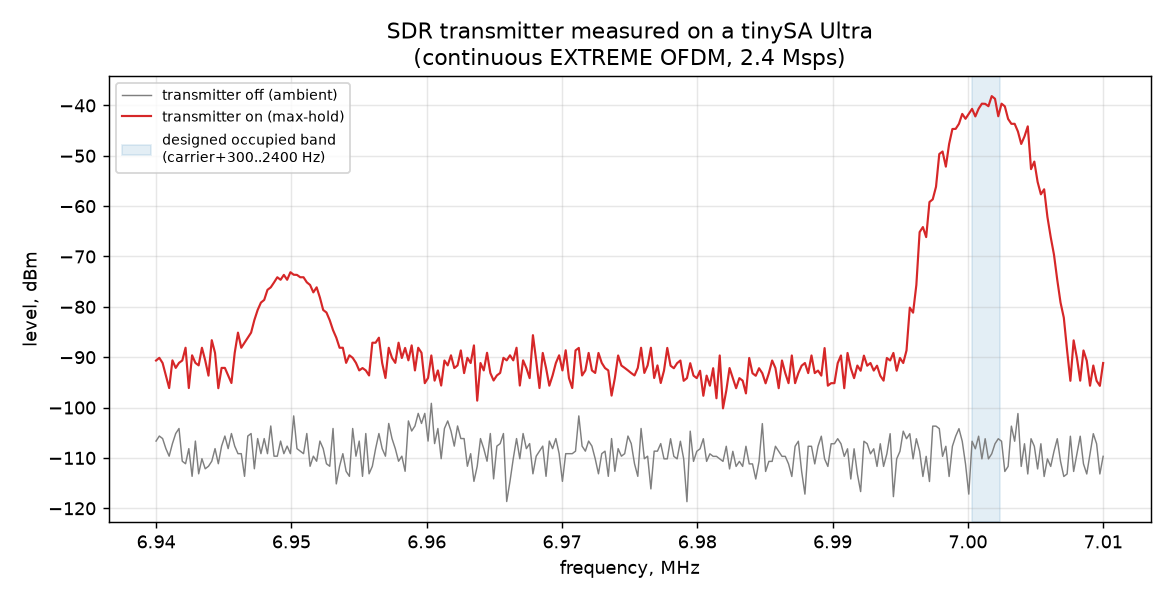
\includegraphics[width=0.92\textwidth]{images/sdr_tx_spectrum.png}
    \caption{The transmitter measured on a tinySA Ultra: continuous
             EXTREME OFDM at 2.4\,Msps, carrier 7.000\,MHz, 3\,kHz RBW.
             The shaded band is the designed occupancy
             (carrier\,$+$\,300\ldots2400\,Hz); the spur at 6.95\,MHz is
             the offset-tuned local oscillator.}
    \label{fig:sdr_tx_spectrum}
\end{figure}

\subsubsection{How Hard the Radio Can Be Driven}

Figure~\ref{fig:sdr_drive_sweep} sweeps the transmit gain and measures,
at each step, the fundamental, the shoulders 5--10\,kHz outside the
occupied band, and the harmonics.  It should be read from the middle
outwards: below VGA 16 the reported shoulders are the \emph{analyser's}
noise floor rather than the transmitter's, because the fundamental is
only $-58$\,dBm.  Above VGA 32 the degradation is real compression,
provoked by the waveform's $\approx$8\,dB PAPR --- at full drive the
shoulders reach $-22$\,dBc and the second harmonic $-38$\,dBc, both
worse than the $-43$\,dBc usually demanded of spurious emissions.

The asymmetry between the two impairments is the practical result: a
low-pass filter removes the harmonics but does nothing about the
shoulders, which are spectral regrowth a few kilohertz from the carrier
and inside any filter's passband.  The usable window with this waveform
is therefore about VGA 16--32, i.e.\ $-42$ to $-24$\,dBm, and real power
has to come from a \emph{linear} external amplifier rather than from
winding this one up --- the same linearity requirement the OFDM
waveform imposes everywhere else in the chain.

\begin{figure}[H]
    \centering
    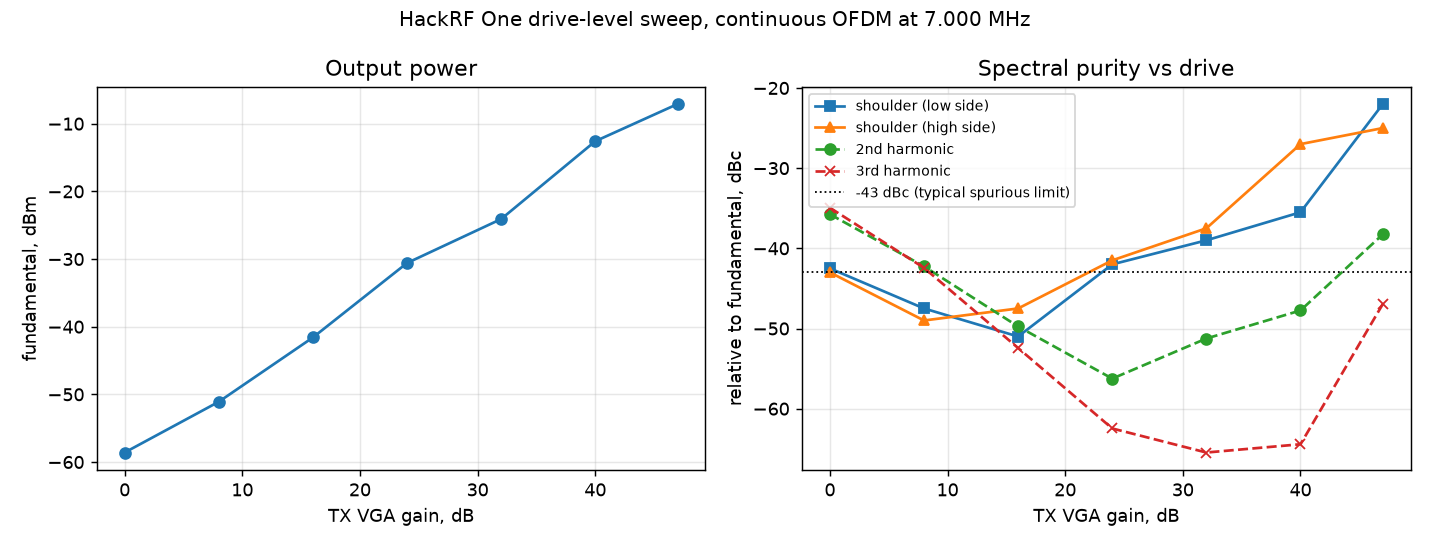
\includegraphics[width=\textwidth]{images/sdr_drive_sweep.png}
    \caption{Drive-level sweep on the HackRF One
             (\texttt{demoapp/sdr\_drive\_sweep.py}): output power, and
             spectral purity relative to the fundamental, against
             transmit gain.  Points below VGA 16 are limited by the
             analyser's noise floor, not by the transmitter.}
    \label{fig:sdr_drive_sweep}
\end{figure}

\subsubsection{Decoding Off the Air}

A half-duplex radio cannot receive its own transmission, so the last
question --- does a receiver actually \emph{decode} this over a real RF
path? --- needs a separate transmitter.  Figure~\ref{fig:sdr_setup_ammod}
shows the one used: a laptop's sound card plays a generated file into an
AM modulator carried by an external generator at 7.000\,MHz, and the
result reaches the SDR through a 40\,dB pad.

AM demands a different detector, for a reason worth stating because it
is a property of the waveform rather than an inconvenience.  The
receiver is single-sideband: it tunes to a \emph{suppressed} carrier and
takes the real part of the baseband.  Present it with a double-sideband
signal and the lower sideband folds onto the upper one; worse, any
frequency error between the generator and the SDR multiplies the audio
by a slow cosine, splitting every subcarrier in two.  The test therefore
recovers the carrier that AM conveniently provides, derotates by it so
the carrier sits at exactly 0\,Hz and zero phase, and only then takes
the real part.  That is classical synchronous detection, and it is why
the decoded CFO in Table~\ref{tab:offair} reads zero: the carrier lock
has already absorbed the error the modem would otherwise estimate.

\begin{figure}[H]
    \centering
    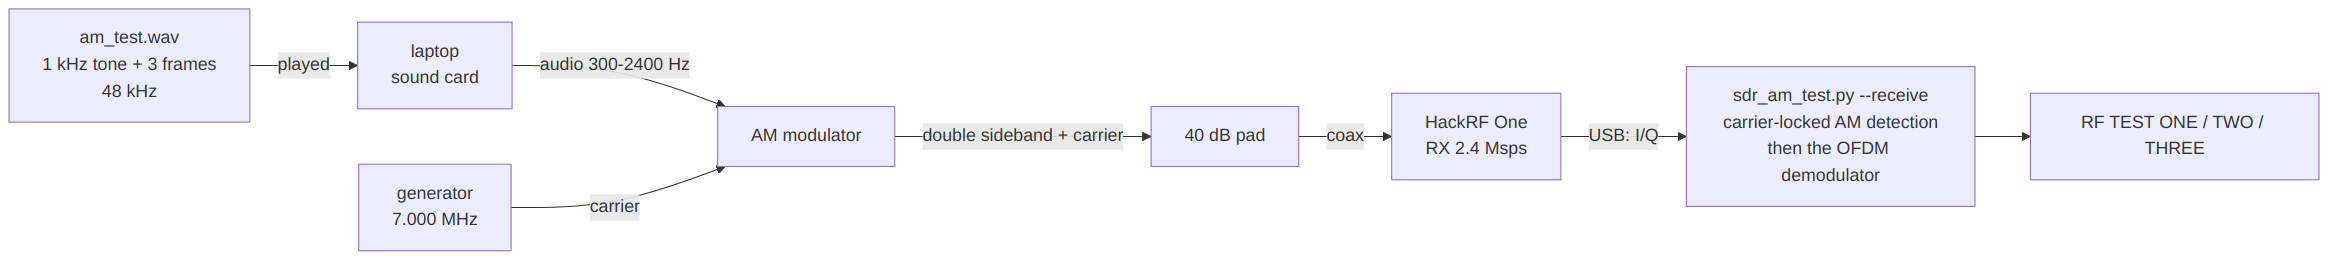
\includegraphics[width=\textwidth]{images/sdr_setup_ammod.png}
    \caption{Off-air receive test: an external AM transmitter feeds the
             SDR through a 40\,dB pad.}
    \label{fig:sdr_setup_ammod}
\end{figure}

\begin{table}[H]
    \centering
    \caption{All three transmitted frames recovered over a 7\,MHz RF
             path (\texttt{results/am\_rx\_offair.wav}).}
    \label{tab:offair}
    \small
    \begin{tabular}{@{}llrr@{}}
    \toprule
    \textbf{Frame} & \textbf{Payload} & \textbf{Length} &
    \textbf{SNR} \\
    \midrule
    NORMAL QPSK 1/2 & \texttt{RF TEST ONE}   & 1.0\,s & $+13.6$\,dB \\
    NORMAL BPSK 1/3 & \texttt{RF TEST TWO}   & 1.8\,s & $+14.4$\,dB \\
    ROBUST BPSK 1/3 & \texttt{RF TEST THREE} & 7.3\,s & $+8.5$\,dB \\
    \bottomrule
    \end{tabular}
\end{table}

Figure~\ref{fig:sdr_waterfall} is what those frames look like as the
demodulator received them.  The analysis FFT is 128 bins at 12\,kHz,
which is exactly the modem's own subcarrier grid, so every row of the
waterfall is one OFDM bin and the structure of
Section~\ref{sec:phy} is directly legible: the Newman tone comb
striping the preamble, then the header, then the data block filling
300--2400\,Hz.  The two NORMAL frames last about a second; the ROBUST
frame occupies 7.35\,s for the same 27 bytes, which is what
$16\times$ tiling costs and buys.  The region boundaries are not
fitted --- they are computed from the decoded header's own modulation,
code rate and length fields, and land on the measured burst to within
15\,ms.

\begin{figure}[H]
    \centering
    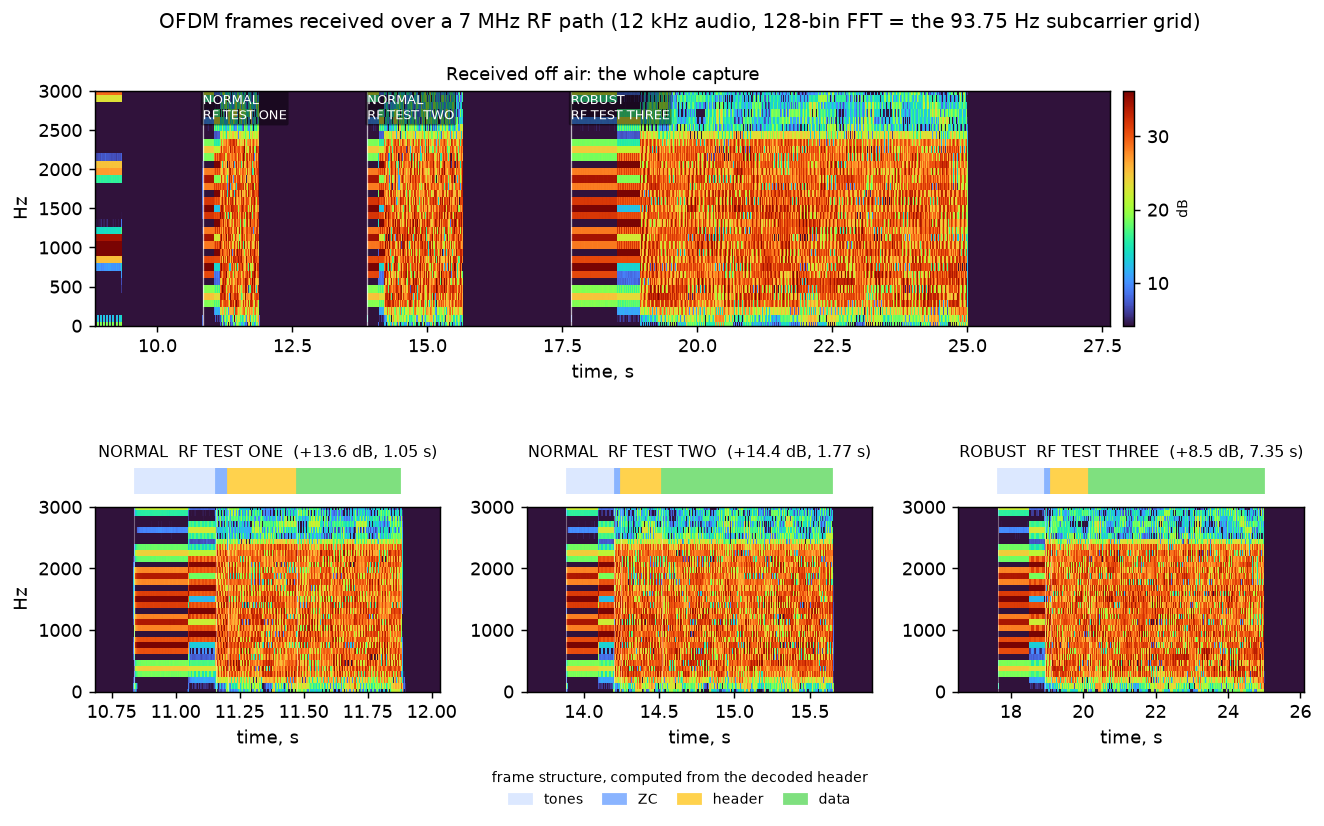
\includegraphics[width=\textwidth]{images/sdr_waterfall.png}
    \caption{Frames received over the air (\texttt{demoapp/sdr\_waterfall.py}
             on \texttt{results/am\_rx\_offair.wav}): the whole capture
             above, each frame close up below with its preamble, header
             and data spans marked.}
    \label{fig:sdr_waterfall}
\end{figure}

Figure~\ref{fig:sdr_waterfall} shows those frames as the demodulator
received them.  The analysis FFT is 128 bins at 12\,kHz, exactly the
modem's own subcarrier grid, so each row is one OFDM bin and the frame
structure of Section~\ref{sec:phy} is directly legible: the Newman tone
comb lighting only a few bins, the Zadoff--Chu symbol closing the
preamble, then the header and the data block filling 300--2400\,Hz.
The spans above each waterfall are computed rather than fitted --- from
the mode's tone-field geometry and the decoded header's own modulation,
code rate and length --- and they land on the measured burst to within
15\,ms.  The comb's end is measurable independently: bin occupancy sits
at 0.17 through the tone fields and jumps to 0.9 at 0.321\,s, against a
predicted 0.320\,s.  It is worth noting that the ZC symbol occupies all
23 carriers, so on a waterfall it resembles data even though it belongs
to the preamble --- which is why it is drawn as its own span.

\begin{figure}[H]
    \centering
    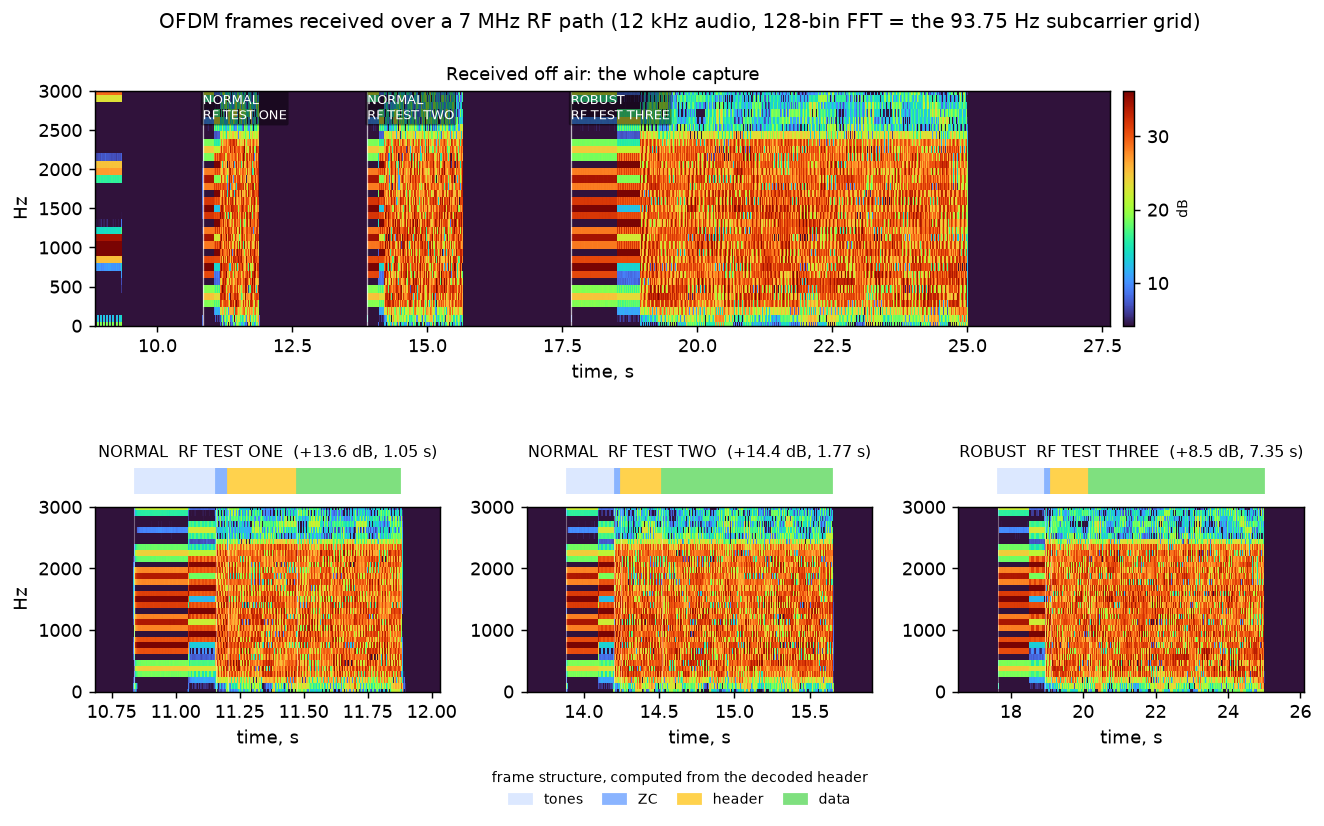
\includegraphics[width=\textwidth]{images/sdr_waterfall.png}
    \caption{Frames received over the air
             (\texttt{demoapp/sdr\_waterfall.py} on
             \texttt{results/am\_rx\_offair.wav}): the whole capture
             above, each frame below with its measured structure.  The
             ROBUST frame carries the same 27 bytes as its NORMAL
             neighbours and occupies 7.35\,s doing it --- what
             $16\times$ tiling costs, and buys.}
    \label{fig:sdr_waterfall}
\end{figure}

Every frame transmitted was recovered, across two link modes and two
modulations, with the mode identified from the preamble root alone ---
the mechanism the whole adaptive ladder depends on, here exercised over
real RF rather than in simulation.  ROBUST reports the lowest SNR by
design: its $16\times$ tiling spreads the same energy over a longer
symbol, so the per-symbol estimate falls while the decoded margin grows.

Two honest qualifications.  The transmitter is an AM modulator rather
than the SDR of the preceding sections, so this validates the receive
chain over RF and not a complete transmit-to-receive loop, which still
wants a second radio.  And a first, coarser scan of the same recording
found only two of the three frames, because it advanced four seconds
after each hit while the demodulator returns one frame per window ---
the miss was in the measurement harness, not the link, which is exactly
the kind of result worth re-checking before blaming the hardware.

\section{Discussion}
\label{sec:discussion}

\subsection{What Binds Performance Now}

\paragraph{The front end, not the code.}  The clearest lesson of the
coding work is that FEC choice stopped mattering before code quality
did: LDPC's 0.7\,dB AWGN advantage compresses to parity end-to-end
because the demodulator's LLR quality is the binding constraint.  The
monotone recalibration recovered 1.5--2\,dB, but a standards-grade
LDPC matrix (802.11n/NR-style~\cite{ieee80211}) \emph{plus} fully
calibrated LLRs would be needed to realise the remaining
$\sim$2\,dB.  Any further sensitivity work should start at the LLR
front end, not the decoder.

\paragraph{Synchronization is the sensitivity frontier.}  Both the
original reproduction gap and the fade-loss analysis point the same
way: at the edge, frames are lost to detection and timing, not to
decoding.  HARQ helps only in the noise-limited regime for exactly
this reason --- a sync-level loss leaves no LLRs to combine.  The
two-board stand made the same point at the \emph{other} end of the
SNR range: broadcast, which cannot retransmit, lost one group in 39 on
a wire reporting $+24.7$\,dB --- a missed acquisition with 25\,dB of
margin, invisible to every acknowledged mode because ARQ had been
quietly repairing it (Section~\ref{sec:cport_bcast}).

\paragraph{Physics caps EXTREME.}  The $64\times$ mode's 0.69\,s
coherent integration assumes a channel coherent over that window
($\lesssim$0.1\,Hz Doppler spread).  This is a physical ceiling, not
an implementation one, and it is why the mode ladder --- rather than
ever-longer integration --- is the right architecture.

\paragraph{Feedback latency at the floor.}  Once a direction falls to
EXTREME, the adaptation loop period is bounded by 25--45\,s frame air
times.  The controller is designed around this (fade-aware filtering,
loss fallback, silence decay), but no tuning can make a 7.8\,bit/s
control loop fast.

\subsection{Limitations}

The channel model, while faithful to the article (and extended with
Rayleigh fading and a physical LO model), is still a simulation; the
measured sensitivities should be planned around with $\sim$3\,dB of
fading margin ($-14\ldots-15$\,dB for EXTREME).  The 16-QAM rungs run
without LLR recalibration (the map is BPSK-trained); a
modulation-specific map is straightforward but unmeasured.  The LDPC
matrix is a from-scratch IRA construction, not a standards matrix.
The project also has no over-the-air validation yet --- the WAV
recordings are transceiver-ready precisely to enable it.  The voice
evaluation of \S\ref{sec:cport_voice} is bounded the same way: the
codec's catastrophic-failure rate was measured on read speech, not on
shack audio, and one non-English trial is an anecdote rather than a
rate.

\subsection{Future Work}

In rough order of expected value: over-the-air testing with real SSB
rigs using the recorded WAVs; a standards-grade LDPC matrix plus
QAM-specific LLR recalibration; porting the fixed receiver's
slew-limited tracker back to the float model (it is measurably
better); pilot reduction or 2-D channel estimation to reclaim carrier
capacity; per-carrier bit-loading on the measured channel estimate;
frame aggregation in the ARQ to amortise preamble overhead at high
rungs; a host-side voice mode over the 250\,bit/s codec evaluated in
\S\ref{sec:cport_voice}, whose remaining question is a failure rate
rather than a bitrate; a 46.875\,Hz-spacing variant for very stable channels; and
shrinking EXTREME's frequency-search range after AFC netting
converges (compute reduction on embedded targets).

\section{Conclusion}
\label{sec:conclusion}

The project set out to reproduce a published amateur-radio OFDM PHY
layer and ended with a complete adaptive communication system.  The
reproduction itself is closed: 44/44 worked examples bit-exact, the
BER/PER figures reproduced, and the sensitivity gap traced to three
specific synchronization defects and eliminated to within 0.3\,dB of a
genie-synchronized bound.  On that foundation, the waveform was
extended an order of magnitude in each direction --- down to
$-17.9$\,dB and 7.8\,bit/s (78\,\% of Shannon capacity at $-20$\,dB)
and up to $+4.7$\,dB and 1059\,bit/s with 16-QAM --- and wrapped in a
link layer that measures everything it can observe and feeds all of it
back: receiver-driven rate adaptation over a 13-rung measured ladder,
CRC-gated HARQ from exported LLRs, learned per-rung sensitivity
offsets, and closed-loop AFC netting of the stations' carrier
frequencies.

Two results deserve emphasis beyond the feature list.  First, the
measured LLR recalibration --- 1.5--2\,dB from correcting the
\emph{shape} of the demodulator's confidence, at zero over-the-air
cost --- illustrates how much sensitivity can hide between a correct
demodulator and a correct decoder.  Second, the fixed-point receiver
matching and then beating the floating-point chain at the sensitivity
edge shows that an RTL-oriented implementation need not be a
degradation; the discipline it forces (bounded scales, division-free
estimation, a tracker instead of a polynomial fit) produced the better
algorithm.

Everything claimed here is regenerable from the repository: the
regression suites are self-verifying, every sensitivity figure has its
sweep script and JSON dump, and the final demonstration is a WAV file
any copy of the receiver decodes blind.  The natural next step is the
one simulation cannot take: the same frames over a real HF path.


% -----------------------------------------------------------------------
% References
% -----------------------------------------------------------------------
\clearpage
\phantomsection
\addcontentsline{toc}{section}{References}
\bibliographystyle{plain}
\bibliography{references}

% -----------------------------------------------------------------------
% Appendices
% -----------------------------------------------------------------------
\clearpage
\appendix

\phantomsection
\addcontentsline{toc}{section}{Appendices}
\begin{center}
    {\Huge\bfseries Appendices\par}
\end{center}
\vspace{1.5em}

\noindent The four appendices below collect verbatim tool output that
would interrupt the main narrative.
Appendix~\ref{app:verify} reproduces the output of the bit-exact
article-reproduction suite (\texttt{verify\_article.py}) referenced in
Section~\ref{sec:results};
Appendix~\ref{app:fixed} reproduces the output of the fixed-point
validation suite (\texttt{fixed\_point.py}) referenced in
Section~\ref{sec:fixed};
Appendix~\ref{app:demo} reproduces the blind-decoded transcript of
the recorded two-station demonstration session
(\texttt{demo\_wav.py}) referenced in Section~\ref{sec:results};
and Appendix~\ref{app:fixeddemo} reproduces the transcript of the same
demonstration running entirely on the fixed-point pipeline at
$+5$\,dB, where the ladder climbs into 16-QAM.

\vspace{1.5em}
\clearpage

\section{Article-Reproduction Suite Output}
\label{app:verify}

Verbatim output of
\texttt{./venv/bin/python experiments/verify\_article.py}: the 44
bit-exact checks against the article's worked examples --- numerology
constants, Base38 callsign and QTH-locator encodings, CRC-8/CRC-16
values, convolutional-code outputs at all four rates,
interleaver/scrambler sequences, and Zadoff--Chu sequence properties.

\lstinputlisting{appendices/verify_article_output.txt}

\section{Fixed-Point Validation Suite Output}
\label{app:fixed}

Verbatim output of
\texttt{./venv/bin/python experiments/fixed\_point.py}: primitive
quality checks (FFT, Hilbert, NCO, CORDIC, integer Viterbi), the
fixed/float TX$\times$RX cross-matrix, the PER comparison table
against the float receiver, and the LDPC / 16-QAM / calibration /
HARQ / ROBUST / EXTREME decode checks referenced in
Section~\ref{sec:fixed}.

\lstinputlisting{appendices/fixed_point_output.txt}

\section{System-Demonstration Transcript}
\label{app:demo}

Verbatim output of
\texttt{./venv/bin/python experiments/demo\_wav.py}: the two-station
session over the fading SSB RF chain
(Section~\ref{sec:results}).  The first block is the simplex
scheduler's air-time log as heard by the passive monitor (per-frame
carrier snapshots include each station's LO drift and AFC trims); the
second block is the \emph{blind-decoded} transcript recovered from the
monitor's WAV audio alone --- mode, modulation and rate from the frame
itself, measured CFO, and the unpacked link-control word
(seq/ack/rung-request/SNR-report) for every decodable frame.  A's and
B's distinct carrier fingerprints ($\approx -18$ and $\approx
-22$\,Hz at the monitor after netting) identify the transmitter of
every frame.  Encrypted-looking payloads are mid-message fragments of
the bulk transfer; \texttt{b'\textbackslash x00'} frames are ACK-only.

\lstinputlisting{appendices/demo_wav_output.txt}

\section{Fixed-Point-Pipeline Demonstration Transcript}
\label{app:fixeddemo}

Verbatim output of
\texttt{./venv/bin/python experiments/demo\_wav.py -{}-phy fixed
-{}-snr 5}: the $+5$\,dB two-station session with both stations and
the passive monitor running the \emph{full fixed-point pipeline}
(Section~\ref{sec:fixed}) --- fixed transmitters, per-mode fixed
receivers with blind mode auto-detection, the integer SNR estimator
driving rate adaptation, and integer HARQ.  The blind transcript shows
the climb from the EXTREME bootstrap through the QPSK rungs into
16-QAM (rungs 9--10 on the air, requests up to rung~11), with the
integer SNR reports in the link-control words and the AFC-netted
carrier fingerprints in the CFO column.

\lstinputlisting{appendices/fixed_demo_output.txt}


\end{document}
